\chapter{Wiadomości wstępne}\label{chapter1}
W niniejszym rozdziale zgromadzone zostały definicje, twierdzenia i~lematy przydatne w~dalszej części rozprawy. Część spośród~nich jest zupełnie standardowa; przy pozostałych podajemy odsyłacze do bibliografii bądź dowody. 

Należy zaznaczyć, że wyniki podane w~tym rozdziale wraz z~dowodami są prawdopodobnie dobrze znane (być może z~wyjątkiem lematu \ref{lem-porządek_bez_promieni_wtw_podzial_barycentryczny}, stwierdzenia \ref{stw-porzadek_bez_promieni_wtw_kompleks_symplicjalny} oraz lematu \ref{lem-permutowanie_podprzestrzeni_a_liczba_lefschetza}) i~nie stanowią oryginalnego wkładu autora, a~jedynie świadczą o~jego trudnościach w~dotarciu do odpowiednich źródeł. 

%====================================================================
%====================================================================
%====================================================================


\section{Różne oznaczenia i~uwagi}
Definiowane pojęcia zapisujemy \textit{tekstem pochyłym}. Przez \textbf{wytłuszczenie} wyróżniamy obowiązujące w~większym fragmencie rozprawy założenia i~oznaczenia.

Zakładamy, że Czytelnik ma podstawową wiedzę z~zakresu algebry, teorii mnogości, topologii (w~tym topologii algebraicznej) oraz teorii kategorii. 

W~rozprawie swobodnie korzystamy z~aksjomatu wyboru, nie czyniąc na ten temat dodatkowych uwag.

Litery $\mathbb{N}$\nomenclature[0a]{$\mathbb{N}$}{zbiór liczb naturalnych}, $\mathbb{Z}$\nomenclature[0b]{$\mathbb{Z}$}{zbiór liczb całkowitych}, $\mathbb{Q}$\nomenclature[0c]{$\mathbb{Q}$}{zbiór liczb wymiernych}, $\mathbb{R}$\nomenclature[0d]{$\mathbb{R}$}{zbiór liczb rzeczywistych} oznaczają kolejno zbiory liczb: naturalnych, całkowitych, wymiernych oraz rzeczywistych (wraz ze standardowymi: topologią, porządkiem i~strukturą algebraiczną na tych zbiorach). 

Moc zbioru $A$~oznaczamy przez $\moc{A}$.\nomenclature[1da]{$\moc{A}$}{moc zbioru $A$} Symbolem $A\big/\mathord{\sim}\ =\left\{[a]_\sim:a\in A\right\}$\nomenclature[1e]{$[x]_\sim$}{klasa abstrakcji elementu $x$~względem relacji równoważności $\sim$} oznaczamy rodzinę klas abstrakcji elementów zbioru $A$~względem relacji równoważności $\sim$~na zbiorze $A$.\nomenclature[1f]{$A\big/\mathord{\sim}$}{zbiór ilorazowy zbioru $A$~względem relacji równoważności $\sim$~na $A$} Jeżeli relacja $\sim$~jest utożsamieniem punktów pewnego niepustego podzbioru $B\subseteq A$, zbiór ilorazowy oznaczamy także przez $A\big/B$. Przy użyciu tego samego symbolu oznaczamy również algebraiczne struktury ilorazowe (np.~grupy ilorazowe).

Literą $\omega$\nomenclature[1g]{$\omega$}{najmniejsza nieskończona liczba porządkowa} oznaczamy najmniejszą nieskończoną liczbę porządkową.

Określenia ,,funkcja'', ,,odwzorowanie'' oraz ,,przekształcenie'' stosujemy wymiennie.

Symbol $\id_X\colon X\to X$\nomenclature[1a]{$\id_X$}{morfizm tożsamościowy obiektu $X$} oznacza morfizm tożsamościowy obiektu $X$. Jeżeli $f\colon X\to Y$ jest funkcją oraz $A\subseteq X$, to przez $f\big|_A\colon A\to Y$\nomenclature[1c]{$f\big\pion_A$}{ograniczenie funkcji $f$~do podzbioru $A$~jej dziedziny} oznaczamy ograniczenie funkcji $f$~do podzbioru $A$. Przez zakrzywioną strzałkę $i\colon X\hookrightarrow Y$\nomenclature[1b]{$i\colon X\hookrightarrow Y$}{funkcja $i\colon X\to Y$ jest włożeniem} oznaczamy fakt, że odwzorowanie $i\colon X\to Y$ jest włożeniem. Jeżeli $A\subseteq X$, to surjekcję $r\colon X\to A$ nazywamy \textit{retrakcją}\index{retrakcja}, o~ile $r(r(x))=r(x)$ dla wszystkich $x\in X$. Jeśli $i\colon A\hookrightarrow X$ oznacza włożenie, to $r\colon X\to A$ jest retrakcją wtedy i~tylko wtedy, gdy $r\circ i=\id_A$.

Dla $n\in\mN$ przez $\S^n$\nomenclature[0g]{$\S^n$}{$n$-wymiarowa sfera jednostkowa} oznaczamy $n$-wymiarową sferę jednostkową $\S^n\subseteq \mathbb{R}^{n+1}$, przez $\D^n$\nomenclature[0e]{$\D^n$}{$n$-wymiarowy, domknięty dysk jednostkowy} domknięty, $n$-wymiarowy dysk jednostkowy $\D^n\subseteq \mathbb{R}^n$, zaś przez $\I$\nomenclature[0f]{$\I$}{domknięty odcinek jednostkowy}~domknięty odcinek jednostkowy $\I=[0,1]\subseteq \mathbb{R}$.

Izomorfizm struktur algebraicznych (grup, pierścieni itp.) oznaczamy symbolem~$\cong$.\nomenclature[1i]{$A \cong B$}{struktury algebraiczne $A, B$ są izomorficzne} Wymiar przestrzeni wektorowej $V$~oznaczamy przez $\dim(V)$.\nomenclature[1g]{$\dim(V)$}{wymiar przestrzeni wektorowej $V$} Symbolem $\bigoplus_{i\in I} V_i$\nomenclature[1h]{ $\bigoplus_{i\in I} V_i$}{suma prosta rodziny przestrzeni wektorowych $\{V_i\}_{i\in I}$} oznaczamy sumę prostą rodziny przestrzeni wektorowych $\{V_i\}_{i\in I}$. Ciąg $V_*=(V_n)_{n\in\mN}$ przestrzeni wektorowych nad tym samym ciałem nazywamy \textit{przestrzenią wektorową z~gradacją}\index{przestrzenzzz wektorowa z gradacjazzz@przestrzeń wektorowa z gradacją}. Jeśli $V_*$, $V'_*$ są przestrzeniami wektorowymi z~gradacją, to ich \textit{homomorfizmem zachowującym gradację}\index{homomorfizm!zachowujazzzcy gradacjezzz@zachowujący gradację} nazywamy ciąg homomorfizmów liniowych $f_*=(f_n\colon V_n\to V_n')_{n\in\mN}$.


Koprodukt obiektów $X, Y$ (zazwyczaj będzie to suma rozłączna zbiorów bądź przestrzeni topologicznych) oznaczamy przez $X\sqcup Y$\nomenclature[1n]{$X\sqcup Y$}{koprodukt obiektów $X, Y$}. Dla oznaczenia koproduktu rodziny obiektów $\left\{X_i\right\}_{i\in I}$ stosujemy symbol $\coprod_{i\in I}X_i$\nomenclature[1o]{$\coprod_{i\in I}X_i$}{koprodukt rodziny obiektów $\{X_i\}_{i\in I}$}, zaś przez $\prod_{i\in I}X_i$\nomenclature[1oa]{$\prod_{i\in I}X_i$}{produkt rodziny obiektów $\{X_i\}_{i\in I}$} oznaczamy produkt tej rodziny.




%====================================================================
%====================================================================
%====================================================================



\section{Matematyka dyskretna}
\subsection{Grafy}
\textit{Grafem prostym} (lub po prostu \textit{grafem})\index{graf!prosty} nazywamy parę $G=(V,E)$ taką, że $V$ jest pewnym zbiorem, zwanym \textit{zbiorem wierzchołków}\index{zbiozzzr@zbiór!wierzcholzzzkozzzw@wierzchołków!grafu} grafu $G$, zaś $E\subseteq\left\{\{v,w\}:v,w\in V\right\}$ jest \textit{zbiorem krawędzi}\index{zbiozzzr@zbiór!krawezzzdzi grafu@krawędzi grafu} tego grafu. 

\textit{Grafem skierowanym}\index{graf!skierowany} nazywamy parę $D=(V,E)$ taką, że $V$ jest pewnym zbiorem, zwanym \textit{zbiorem wierzchołków} grafu skierowanego $D$, zaś $E\subseteq V\times V$ jest \textit{zbiorem (skierowanych) krawędzi} grafu skierowanego $D$. Jeżeli $(v,w)\in E$, to mówimy, że krawędź $(v,w)$ \textit{wychodzi z~wierzchołka $v$} i~\textit{wchodzi do wierzchołka $w$}.

\begin{uw}\label{uw-o-utozsamieniu}
Graf prosty $G=(V,E)$ możemy utożsamiać z~grafem skierowanym $G'=(V,E')$, którego zbiorem krawędzi jest $E'=\{(v,w):\{v,w\}\in E\}$. Z~drugiej strony graf skierowany $D=(W,F)$, którego zbiór krawędzi $F\subseteq W\times W$ jest symetryczną relacją dwuargumentową na zbiorze $W$, możemy utożsamiać z~grafem prostym $D'=(W,F')$ o~zbiorze krawędzi $F'=\{\{v,w\}:(v,w)\in F\}$.
\end{uw}

W~oznaczeniach często pomijać będziemy zbiory wierzchołków i~krawędzi; przykładowo, pisząc $v\in G$, $\{v,w\}\in G$ mamy na myśli przynależność wierzchołka $v$~do zbioru wierzchołków grafu $G$ oraz krawędzi $\{v,w\}$~do zbioru jego krawędzi.

\textit{Ścieżką}\index{szzzciezzzzka w grafie@ścieżka w grafie} długości $n$~w~grafie skierowanym $D$~prowadzącą z~wierzchołka $v_0$~do wierzchołka $v_n$~nazywamy taki skończony ciąg wierzchołków $(v_0,\ldots,v_n)$ tego grafu, że krawędź $(v_i,v_{i+1})\in D$ dla wszystkich $i=0,\ldots,n-1$. \textit{Nieskończoną ścieżką}\index{szzzciezzzzka w grafie@ścieżka w grafie!nieskonzzzczona@nieskończona} w~grafie skierowanym $D$ nazywamy taki nieskończony ciąg wierzchołków $(v_i)_{i\in\mN}$ tego grafu, że $(v_i,v_{i+1})\in D$ dla wszystkich $i\in\mN$. Mówimy, że ścieżka (skończona lub nie) w~grafie skierowanym $D$ jest \textit{prosta}\index{szzzciezzzzka w grafie@ścieżka w grafie!prosta}, o~ile jej wierzchołki są parami różne. Skończoną ścieżkę prostą $(v_0,\ldots,v_n)$ taką, że $n\geq 1$ oraz $(v_n,v_0)\in D$, nazywamy \textit{cyklem}\index{cykl w~grafie}.

Dzięki utożsamieniu z~uwagi \ref{uw-o-utozsamieniu} dobrze określone są również pojęcia ścieżki, ścieżki prostej oraz cyklu w~grafie prostym.

Graf skierowany $D'=(V',E')$ nazywamy \textit{podgrafem}\index{podgraf} grafu skierowanego $D=(V,E)$, o~ile $V'\subseteq V$ oraz $E'\subseteq E$. Jeżeli ponadto $E'=E\cap \left(V'\times V'\right)$, to $D'$~nazywamy podgrafem \textit{indukowanym}\index{podgraf!indukowany} na zbiorze wierzchołków $V'\subseteq V$. 

Jeżeli $D=(V,E)$ jest grafem skierowanym oraz $W\subseteq V$, to podgraf grafu $D$~indukowany na zbiorze wierzchołków $V\smallsetminus W$ oznaczamy przez $D-W$.\nomenclature[2c]{$D-A$}{podgraf grafu skierowanego $D$~indukowany na dopełnieniu podzbioru $A$~zbioru wierzchołków tego grafu}


Mówimy, że graf prosty $G$~jest \textit{spójny}\index{graf!spozzzjny@spójny}, jeżeli dla wszystkich wierzchołków $v,w\in G$ istnieje ścieżka w~$G$~prowadząca z~$v$~do~$w$. \textit{Składową spójności}\index{sklzzzadowa spozzzjnoszzzci@składowa spójności!grafu} grafu $G$~nazywamy każdy maksymalny (w~sensie relacji bycia podgrafem) spójny podgraf tego grafu. Graf prosty $G$~nazywamy \textit{drzewem}\index{drzewo}, o~ile jest spójny i~nie zawiera cykli długości $\geq 2$.

Mówimy, że graf skierowany $D$ jest \textit{lokalnie skończony}\index{graf!lokalnie skonzzzczony@lokalnie skończony}, o~ile dla każdego wierzchołka $v\in D$ zbiór $\{w\in D:(v,w)\in D\text{ lub } (w,v)\in D\}$ jest skończony. 

\begin{lem}[K{\"o}niga, {\cite[Lemma 8.1.2]{Diestel10}}]\label{konig}
Niech $D$~będzie lokalnie skończonym grafem skierowanym, zaś $v\in D$ wierzchołkiem tego grafu. Jeżeli zbiór tych wierzchołków $w\in D$, dla których istnieje ścieżka w~$D$~prowadząca z~$v$~do $w$, jest nieskończony, to istnieje nieskończona ścieżka prosta w~$D$.
\end{lem}

Niech $D=(V,E)$ będzie grafem skierowanym. \textit{Skojarzeniem}\index{skojarzenie} w~$D$ nazywamy taki zbiór krawędzi $M\subseteq E$, że dla każdego wierzchołka $v\in V$ istnieje co najwyżej jedna krawędź $(w_1,w_2)\in M$ o~tej własności, że $v=w_1$ lub $v=w_2$.

Interesujące z~punktu widzenia niniejszej rozprawy wprowadzenie do teorii grafów zawiera książka Diestela \cite{Diestel10}, której znacząca część poświęcona jest nieskończonym grafom.



%--------------------------------------------------------------------
%--------------------------------------------------------------------
%--------------------------------------------------------------------




\subsection{Częściowe porządki i~kraty}
Niech $P$~będzie zbiorem. Dwuargumentową relację $\leq\ \subseteq P\times P$ nazywamy \textit{relacją quasi-porządku}\index{relacja!quasi-porzazzzdku@quasi-porządku} na $P$, o~ile jest ona zwrotna i przechodnia; jeżeli relacja ta jest dodatkowo słabo antysymetryczna (tzn.~dla wszystkich $p,q\in P$ jeśli $p\leq q$ oraz $q\leq p$, to $p=q$), nazywamy ją \textit{relacją częściowego porządku}.\index{relacja!czezzzszzzciowego porzazzzdku@częściowego porządku}

\textit{Quasi-porządkiem} (lub \textit{zbiorem quasi-uporządkowanym})\index{quasi-porzazzzdek@quasi-porządek}\index{zbiozzzr@zbiór!quasi-uporzazzzdkowany@quasi-uporządkowany|see{quasi-porządek}} nazywamy parę $(P,\leq)$ taką, że $P$~jest zbiorem, zaś $\leq\ \subseteq P\times P$ jest relacją quasi-porządku na $P$. \textit{Częściowym porządkiem}\index{czezzzszzzciowy porzazzzdek@częściowy porządek} (lub \textit{zbiorem częściowo uporządkowanym}\index{zbiozzzr@zbiór!czezzzszzzciowo uporzazzzdkowany@częściowo uporządkowany|see{częściowy porządek}}, albo po prostu \textit{porządkiem}) nazywamy parę $(P,\leq)$ taką, że $\leq$~jest relacją częściowego porządku na zbiorze $P$. Niech $(P,\leq)$ będzie quasi-porządkiem. Przez $<\ \subseteq P\times P$ oznaczamy relację $<\ =\ \leq\smallsetminus \id_P$. W~oczywisty sposób definiujemy relacje $\geq$~i~$>$. \textit{Quasi-porządkiem dualnym}\index{quasi-porzazzzdek@quasi-porządek!dualny}\index{czezzzszzzciowy porzazzzdek@częściowy porządek!dualny} do $(P,\leq)$ nazywamy quasi-porządek $(P,\geq)$. Przez $\sim\ \subseteq P\times P$\nomenclature[4ba]{$p\sim q$}{elementy $p$, $q$~częściowego porządku są porównywalne} oznaczamy relację \textit{porównywalności}\index{relacja!porozzzwnywalnoszzzci@porównywalności}\index{porozzzwnywalnoszzzczzz@porównywalność}, czyli $\sim\ =\ \leq\ \cup\ \geq$

Ustalmy zbiór częściowo uporządkowany $(P,\leq)$. Jeżeli $\sim\ =P\times P$, to mówimy, że $(P,\leq)$~jest \textit{zbiorem liniowo uporządkowanym}\index{zbiozzzr@zbiór!liniowo uporzazzzdkowany@liniowo uporządkowany|see{łańcuch}}\index{czezzzszzzciowy porzazzzdek@częściowy porządek!liniowy|see{łańcuch}} (lub \textit{liniowym porządkiem}, albo \textit{łańcuchem}\index{lzzzanzzzcuch@łańcuch}). Jeśli natomiast $\leq=\id_P$, to $(P,\leq)$ nazywamy \textit{antyłańcuchem}\index{antylzzzanzzzcuch@antyłańcuch}. \textit{Liniowym rozszerzeniem}\index{rozszerzenie liniowe} częściowego porządku $(P,\leq)$ nazywamy taki zbiór liniowo uporządkowany $P^*=(P,\leq^*)$, że $\leq\ \subseteq\ \leq^*$.

Jeśli $Q\subseteq P$, to relacja częściowego porządku $\leq$~na $P$~indukuje relację $\leq\!\big |_Q$ na zbiorze $Q$ w~oczywisty sposób: dla $q,q'\in Q$ zachodzi $q\leq\!\big |_Q q'$, o~ile $q\leq q'$. Para $(Q,\leq\!\big |_Q)$ jest częściowym porządkiem, zwanym \textit{podzbiorem częściowo uporządkowanym}\index{podzbiozzzr@podzbiór!czezzzszzzciowo uporzazzzdkowany@częściowo uporządkowany} porządku $(P,\leq)$. Mówimy, że $Q\subseteq P$ jest \textit{łańcuchem (antyłańcuchem) w~$P$}, o~ile $(Q,\leq\big |_Q)$ jest łańcuchem (antyłańcuchem). Jeśli nie będzie to prowadziło do nieporozumień, porządek $(Q,\leq\!\big |_Q)$ oznaczać będziemy przez $(Q,\leq)$.

\textit{Elementem maksymalnym}\index{element!maksymalny} w~podzbiorze $A\subseteq P$ nazywamy każdy element $a\in A$ o~tej własności, że nie istnieje element $b\in A$ taki, że $b>a$. Zbiór elementów maksymalnych w~zbiorze $A\subseteq P$~oznaczamy przez $\max(A)$\nomenclature[4e]{$\max(A)$}{zbiór elementów maksymalnych w~$A$, albo element największy w~tym zbiorze}. Dualnie definiujemy \textit{element minimalny}\index{element!minimalny} oraz zbiór $\min(A)$\nomenclature[4ea]{$\min(A)$}{zbiór elementów minimalnych w~$A$, albo element najmniejszy w~tym zbiorze}. \textit{Elementem największym}\index{element!najwiezzzkszy@największy} w~$A$ nazywamy taki element $a\in A$, że $a\geq b$ dla wszystkich $b\in A$. Dualnie definiujemy \textit{element najmniejszy}\index{element!najmniejszy}. Jeśli zbiór $A$~ma~element największy (najmniejszy), oznaczamy go tym samym co wyżej symbolem $\max(A)$ (odpowiednio $\min(A)$); jego właściwe znaczenie wynikać będzie z~kontekstu. \textit{Kresem górnym}\index{kres gozzzrny (dolny)@kres górny (dolny)} podzbioru $A\subseteq P$, oznaczanym przez $\sup(A)$,\nomenclature[4f]{$\sup(A)$}{kres górny zbioru $A$} nazywamy najmniejszy element zbioru $\{p\in P:p\geq a \text{ dla wszystkich } a\in A\}$, o~ile element taki istnieje. Dualnie definiujemy \textit{kres dolny} zbioru $A$, oznaczany przez $\inf(A)$\nomenclature[4fa]{$\inf(A)$}{kres dolny zbioru $A$}. Kresy górny i~dolny zbioru $\{p,q\}\subseteq P$ oznaczamy odpowiednio przez $p\lor q$ oraz~$p\land q$. \nomenclature[4g]{$p\lor q$}{kres górny zbioru dwuelementowego $\{p,q\}$}\nomenclature[4ga]{$p\land q$}{kres dolny zbioru dwuelementowego $\{p,q\}$}

Częściowy porządek $(P,\leq)$~nazywamy \textit{łańcuchowo zupełnym}\index{czezzzszzzciowy porzazzzdek@częściowy porządek!lzzzanzzzcuchowo zupelzzzny@łańcuchowo zupełny}, o~ile dla każdego podzbioru liniowo uporządkowanego $C\subseteq P$ istnieją jego kresy $\sup(C)$ oraz $\inf(C)$.

Niech $(P,\leq_P),(Q,\leq_Q)$ będą częściowymi porządkami. Mówimy, że funkcja $f\colon P\to Q$ \textit{zachowuje porządek}\index{odwzorowanie!zachowujazzzce porzazzzdek@zachowujące porządek}, jeżeli dla wszystkich $p,p'\in P$ takich, że \mbox{$p\leq_P p'$}, zachodzi $f(p)\leq_Q f(p')$. \textit{Izomorfizmem} częściowych porządków nazywamy bijekcję $f\colon P\to Q$ zachowującą porządek i~taką, że funkcja do niej odwrotna $f^{-1}\colon Q\to P$ zachowuje porządek.

O~ile nie będzie to prowadziło do nieporozumień, częściowy porządek $(P,\leq)$ oznaczać będziemy odtąd krótko przez $P$. Relacje częściowego porządku na różnych zbiorach oznaczać będziemy tym samym symbolem $\leq$~(a~niekiedy również symbolami mu podobnymi, np.~$\sqsubseteq$, $\leq^*$).

\begin{lem}[{\cite[Proposition 4.1.6]{Schroder03}}]\label{retrakt_lanc_zup_jest_lanc_zup}
Jeżeli $P$~jest łańcuchowo zupełnym częściowym porządkiem, zaś $r\colon P\to Q$ jest zachowującą porządek retrakcją, to częściowy porządek $Q$~jest łańcuchowo zupełny.
\end{lem}

Niech $P$ będzie częściowym porządkiem, zaś $p\in P$ jego elementem. Przyjmujemy oznaczenia 
\begin{align*}p\mathord{\downarrow}_P&=\{q\in P:q\leq p\},& p\mathord{\uparrow}_P&=\{q\in P:q\geq p\},\\ \hat{p}\mathord{\downarrow}_P&=p\mathord{\downarrow}_P\smallsetminus\{p\},& \hat{p}\mathord{\uparrow}_P&=p\mathord{\uparrow}_P\smallsetminus\{p\},\end{align*}
 przy czym, o~ile nie będzie to prowadziło do niejednoznaczności, będziemy w~zapisie tych symboli pomijać $P$, tzn. pisać $p\mathord{\downarrow}$, $\hat{p}\mathord{\uparrow}$, itd.\nomenclature[4c]{$p\cofka\downarrow_P$}{zbiór elementów częściowego porządku $P$~mniejszych lub równych $p$}\nomenclature[4d]{$\hat{p}\cofka\downarrow_P$}{zbiór elementów częściowego porządku $P$~mniejszych od $p$}\nomenclature[4ca]{$p\cofka\uparrow_P$}{zbiór elementów częściowego porządku $P$~większych lub równych $p$}\nomenclature[4da]{$\hat{p}\cofka\uparrow_P$}{zbiór elementów częściowego porządku $P$~większych od $p$}

Niech $C=\{p_0,p_1,\ldots,p_n\}\subseteq P$ będzie niepustym, skończonym łańcuchem w~częściowym porządku $P$. Liczbę $n=\moc{C}-1$~nazywamy \textit{długością}\index{dlzzzugoszzzczzz lzzzancucha@długość łańcucha}\index{lzzzanzzzcuch@łańcuch!dlzzzugoszzzci n@długości $n$} łańcucha $C$. Mówimy, że częściowy porządek $P$~jest \textit{skończonej wysokości} \index{czezzzszzzciowy porzazzzdek@częściowy porządek!skonzzzczonej wysokoszzzci@skończonej wysokości}, jeżeli istnieje $n\in\mN$ takie, że wszystkie łańcuchy w~$P$~mają długość równą co najwyżej $n$.

Mówimy, że $P$ jest częściowym porządkiem \textit{z gradacją}\index{czezzzszzzciowy porzazzzdek@częściowy porządek!z gradacjazzz@z gradacją}, jeżeli dla każdego $p\in P$ wszystkie maksymalne (w sensie inkluzji) łańcuchy w~zbiorze $p\mathord{\downarrow}$ są skończone i~mają tę samą długość. Ogólniej, jeżeli istnieje (skończone) maksimum długości łańcuchów zawartych w~zbiorze $p\mathord{\downarrow}$, to nazywamy je \textit{rangą elementu $p$}\index{ranga!elementu czezzzszzzciowego porzazzzdku@elementu częściowego porządku}~i~oznaczamy symbolem $\rk(p)$\nomenclature[4o]{$\rk(p)$}{ranga elementu $p$~częściowego porządku}. Mówimy, że częściowy porządek $P$:\begin{compactitem}
\item[---] jest \textit{dobrze ufundowany}\index{czezzzszzzciowy porzazzzdek@częściowy porządek!dobrze ufundowany}, jeżeli każdy niepusty podzbiór $A\subseteq P$ ma element minimalny;
\item[---] jest \textit{porządkiem z~rangą}\index{czezzzszzzciowy porzazzzdek@częściowy porządek!z rangazzz@z rangą}, jeżeli dla każdego elementu $p\in P$ zdefiniowana jest jego ranga $\rk(p)$; 
\item[---] ma \textit{skończone ideały główne}\index{czezzzszzzciowy porzazzzdek@częściowy porządek!o skonzzzczonych idealzzzach glzzzozzzwnych@o skończonych ideałach głównych}, jeżeli dla każdego $p\in P$ zbiór $p\mathord{\downarrow}$ jest skończony.
\end{compactitem}

Zauważmy, że częściowy porządek $P$~jest dobrze ufundowany wtedy i~tylko wtedy, gdy nie zawiera \textit{nieskończonego łańcucha zstępującego}\index{lzzzanzzzcuch@łańcuch!nieskonzzzczony zstezzzpujazzzcy@nieskończony zstępujący}, czyli podzbioru izomorficznego ze~zbiorem ujemnych liczb całkowitych ze standardową relacją porządkującą. Jeżeli porządek $P$~ma skończone ideały główne, to jest porządkiem z~rangą, zaś każdy porządek z~rangą jest dobrze ufundowany. Dobrze ufundowany liniowy porządek nazywamy \textit{dobrym porządkiem}.\index{czezzzszzzciowy porzazzzdek@częściowy porządek!dobry}

Podzbiór $A$~liniowego porządku $P$~nazywamy jego \textit{odcinkiem początkowym}\index{odcinek poczazzztkowy@odcinek początkowy}, jeżeli $a\mathord{\downarrow}_{P}\subseteq A$ dla każdego $a\in A$.

Niech $(P,\leq_P),(Q,\leq_Q)$ będą częściowymi porządkami. Przez $P\oplus Q$\nomenclature[4i]{$P\oplus Q$}{suma leksykograficzna częściowych porządków $P$, $Q$} oznaczamy częściowy porządek $(P\sqcup Q,\leq)$, którego relacja porządkująca jest sumą \[\leq\ =\ \leq_P\ \cup\ \leq_Q\ \cup\ \{(p,q):p\in P, q\in Q\}.\] Innymi słowy, $a\leq b$ dla $a,b\in P\oplus Q$ wtedy, gdy oba elementy $a$, $b$ należą do któregoś ze zbiorów $P$, $Q$ oraz $a$~jest mniejsze lub równe $b$~w~tym zbiorze, lub gdy $a\in P$ oraz $b\in Q$. Porządek $P\oplus Q$ nazywamy \textit{sumą leksykograficzną}\index{suma leksykograficzna} porządków $P, Q$.

Element $p\in P$ nazywamy \textit{pokryciem górnym}\index{pokrycie gozzzrne (dolne)@pokrycie górne (dolne)} elementu $q\in P$ (zaś $q$ nazywamy \textit{pokryciem dolnym} $p$), jeżeli $p>q$ oraz nie istnieje $r\in P$ takie, że $p>r>q$. Piszemy wówczas $p\succ q$\nomenclature[4a]{$p\succ q$}{element $p$~jest pokryciem górnym elementu $q$} (lub $q\prec p$). Przez zapis $p\succeq q$\nomenclature[4b]{$p\succeq q$}{element $p$~jest pokryciem górnym elementu $q$~lub jest mu równy} (lub $q\preceq p$) rozumiemy, że $p\succ q$ lub $p=q$.

Przez $\mH(P)=(P,\succ)$\nomenclature[6h]{$\mH(P)$}{diagram Hassego częściowego porządku $P$} oznaczamy graf skierowany zwany \textit{diagramem Hassego}\index{diagram Hassego} częściowego porządku $P$. Rysując diagram Hassego przyjmuje się często konwencję, że elementy mniejsze w~porządku $P$~znajdują się niżej niż większe, co pozwala pominąć na rysunku groty strzałek oznaczające orientacje krawędzi. Przykładowy diagram Hassego, narysowany zgodnie z~tą zasadą, przedstawia rysunek \ref{fig-diagram_hassego}.

\begin{figure}[h]
\[\xymatrix{
& x_5\ar@{-}[d]\ar@{-}[ddl]\\
& x_3\ar@{-}[d]\ar@{-}[dr] & x_4\ar@{-}[d]\ar@{-}[dl]\\
x_0 & x_1 & x_2
}\]
\caption{Diagram Hassego częściowego porządku na zbiorze $\{x_0,\ldots,x_5\}$ zadanego przez  $x_0<x_5$, $x_1<x_3$, $x_1<x_4$, $x_1<x_5$, $x_2<x_3$, $x_2<x_4$, $x_2<x_5$, $x_3<x_5$.}\label{fig-diagram_hassego}
\end{figure}

Jeśli zbiór częściowo uporządkowany $P$ nie zawiera podzbioru izomorficznego ze zbiorem~\mbox{$\mN\cup\{\infty\}$} ze standardowym porządkiem lub z~porządkiem do niego dualnym, to $P$ jest jednoznacznie wyznaczony przez swój diagram Hassego $\mH(P)$. Dla dowolnych częściowych porządków nie jest to jednak prawdą (np. dla $P=\mathbb{R}$ ze zwykłym porządkiem).

Graf skierowany $\Comp(P)=(P,\sim)$\nomenclature[6g]{$\Comp(P)$}{graf porównywalności częściowego porządku $P$} nazywamy \textit{grafem porównywalności}\index{graf!porozzzwnywalnoszzzci@porównywalności} częściowego porządku $P$. Ponieważ $\sim$ jest relacją symetryczną, $\Comp(P)$ możemy, wobec uwagi \ref{uw-o-utozsamieniu}, traktować jako graf prosty.
Porządek $P$~nazywamy \textit{spójnym}\index{czezzzszzzciowy porzazzzdek@częściowy porządek!spozzzjny@spójny}, jeżeli graf $\Comp(P)$~jest spójny; w~oczywisty sposób definiujemy \textit{składowe spójności}\index{sklzzzadowa spozzzjnoszzzci@składowa spójności!czezzzszzzciowego porzazzzdku@częściowego porządku} porządku $P$. Mówimy, że częściowy porządek $P$~jest \textit{lokalnie skończony}\index{czezzzszzzciowy porzazzzdek@częściowy porządek!lokalnie skonzzzczony@lokalnie skończony}, o~ile graf $\Comp(P)$ jest lokalnie skończony.

Nieskończoną ścieżkę prostą w~grafie porównywalności $\Comp(P)$ częściowego porządku $P$~nazywamy \textit{promieniem}\index{promienzzz@promień!w czeszzzciowym porzazzzdku@w częściowym porządku} w~$P$. Jeżeli $P$~nie zawiera promienia, to mówimy, że jest częściowym porządkiem \textit{bez promieni}\index{czezzzszzzciowy porzazzzdek@częściowy porządek!bez promieni} (por.~analogiczne definicje dla grafów~\cite{Schmidt83,Halin98}; pod inną nazwą porządki bez promieni rozważał wcześniej autor rozprawy \cite{Kukiela10,Kukiela10a}). Oczywiście, jeśli $P$~jest porządkiem bez promieni, to nie zawiera nieskończonego łańcucha.

\textit{Kratą}\index{krata} nazywamy taki częściowy porządek $L$, w~którym dla wszystkich elementów $p,q\in L$ istnieją kresy $p\lor q$ oraz $p\land q$. Wynika stąd, że w~kracie $L$ istnieją kresy $\sup(A)$ oraz $\inf(A)$ każdego skończonego, niepustego zbioru $A\subseteq L$. Kratę $L$~nazywamy \textit{zupełną}\index{krata!zupelzzzna@zupełna}, o~ile dla każdego podzbioru $A\subseteq L$ istnieją w~$L$~kresy $\sup(A)$ oraz $\inf(A)$.

\begin{lem}[{\cite[Proposition 5.1.7]{Schroder03}}]\label{lem-krata_bez_nsk_lancuchow_jest_zupelna}
Krata jest zupełna wtedy i~tylko wtedy, gdy jest łańcuchowo zupełna. W~szczególności, każda krata nie zawierająca nieskończonego łańcucha jest zupełna.
\end{lem}

Jeżeli krata $L$~ma element największy, który oznaczamy przez $\ltop_L$, to $L$ nazywamy \textit{kratą z~jedynką}\index{krata!z zerem i~jedynkazzz@z zerem i jedynką}. Element najmniejszy kraty $L$, o~ile istnieje, oznaczamy symbolem $\lbottom_L$ i~mówimy w~tej sytuacji, że $L$ jest \textit{kratą z~zerem}.\nomenclature[4h]{$\ltop_L$, $\lbottom_L$}{największy i~najmniejszy element kraty $L$} Zauważmy, że każda zupełna krata ma zero i~jedynkę.

Jeśli $L$~jest kratą z~zerem i~jedynką, to \textit{ściętą kratą}\index{krata!szzzciezzzta@ścięta} powstałą z~$L$~nazywamy częściowy porządek $\check{L}=L\smallsetminus\{\ltop_L,\lbottom_L\}$.

Mówimy, że element $p$~kraty $L$~z~zerem i~jedynką jest \textit{dopełnieniem}\index{dopelzzznienie elementu kraty@dopełnienie elementu kraty} elementu $q\in L$, jeżeli $p\lor q=\ltop_L$ oraz $p\land q=\lbottom_L$. Kratę $L$~z~zerem i~jedynką nazywamy \textit{kratą bez dopełnień}\index{krata!bez dopelzzznienzzz@bez dopełnień}, jeśli istnieje element $p\in \check{L}$, który nie ma dopełnienia w~$L$. 

\textit{Podzbiorem początkowym}\index{podzbiozzzr@podzbiór!poczazzztkowy@początkowy} w~częściowym porządku $P$~nazywamy taki podzbiór $Q\subseteq P$, że dla każdego elementu $p\in P$~zbiór $p\mathord{\downarrow}\cap\ Q\not=\emptyset$. Dualnie definiujemy \textit{podzbiór końcowy}\index{podzbiozzzr@podzbiór!konzzzcowy@końcowy}. Mówimy, że krata $L$~z~zerem i~jedynką \textit{ma mocne dopełnienia}, jeśli dla każdego elementu $p\in\check{L}$, każdego podzbioru początkowego $Q\subseteq \check{L}$ i~każdego podzbioru końcowego $R\subseteq \check{L}$ istnieją skończone podzbiory $Q_p\subseteq Q$, $R_p\subseteq R$ takie, że $\sup(Q_p)$ oraz $\inf(R_p)$ są dopełnieniami elementu $p$. W~przeciwnym wypadku mówimy, że $L$~jest kratą \textit{bez mocnych dopełnień}\index{krata!bez mocnych dopelzzznienzzz@bez mocnych dopełnień}. Nietrudno spostrzec, że jeśli krata $L$~nie zawiera nieskończonego łańcucha, to ma mocne dopełnienia wtedy i~tylko wtedy, gdy dla każdego elementu $p\in\check{L}$ istnieje jego dopełnienie będące kresem górnym pewnego zbioru $Q_p\subseteq \min(\check{L})$ oraz dopełnienie będące kresem dolnym pewnego zbioru $R_p\subseteq \max(\check{L})$.





%===================================================================
%===================================================================
%===================================================================



\section{Topologia ogólna}\label{sec-top_ogolna}
\textbf{Do końca podrozdziału \ref{sec-top_ogolna} niech $X, Y$ oznaczają przestrzenie topologiczne.}

Symbolem $X \approx Y$\nomenclature[1j]{$X \approx Y$}{przestrzenie topologiczne $X, Y$ są homeomorficzne} oznaczamy istnienie homeomorfizmu pomiędzy przestrzeniami $X, Y$. Domknięcie i~wnętrze podzbioru $A\subseteq X$ oznaczamy odpowiednio przez $\overline{A}^X$\nomenclature[1p]{$\overline{A}$,\ \ $\overline{A}^{X}$}{domknięcie zbioru $A$ (w~przestrzeni topologicznej $X$)}~oraz $\Int_X(A)$\nomenclature[1q]{$\Int{A}$,\ \ $\Int_X{A}$}{wnętrze zbioru $A$ (w~przestrzeni topologicznej $X$)}; jeżeli z~kontekstu wynika, w~jakiej przestrzeni rozważamy operację domknięcia lub wnętrza, piszemy krótko $\overline{A}$, $\Int(A)$.

Przestrzeń topologiczną $X$~nazywamy \textit{łukowo spójną}\index{przestrzenzzz topologiczna@przestrzeń topologiczna!lzzzukowo spozzzjna@łukowo spójna}, jeżeli dla każdej pary elementów $(x,y)\in X\times X$ istnieje ciągłe przekształcenie $f\colon \I\to X$ takie, że $f(0)=x$ oraz $f(1)=y$. Mówimy, że $X$~jest \textit{lokalnie łukowo spójna}\index{przestrzenzzz topologiczna@przestrzeń topologiczna!lokalnie lzzzukowo spozzzjna@lokalnie łukowo spójna}, jeśli dla każdego elementu $x\in X$ i~każdego jego otwartego otoczenia $U\subseteq X$ istnieje otwarte otoczenie $V\subseteq U$ punktu $x$~będące przestrzenią łukowo spójną. \textit{Składową łukowej spójności}\index{sklzzzadowa lzzzukowej spozzzjnoszzzci@składowa łukowej spójności} przestrzeni $X$~nazywamy każdy maksymalny łukowo spójny podzbiór tej przestrzeni.

Przez \textit{zwartą}\index{przestrzenzzz topologiczna@przestrzeń topologiczna!zwarta} przestrzeń topologiczną rozumiemy przestrzeń, której dowolne pokrycie otwarte zawiera skończone podpokrycie; nie zakładamy, że przestrzeń ta jest Hausdorffa. Mówimy, że przestrzeń $X$ jest \textit{$\sigma$-zwarta}\index{przestrzenzzz topologiczna@przestrzeń topologiczna!sigma-zwarta@$\sigma$-zwarta}, o~ile $X$ jest sumą przeliczalnej rodziny swoich zwartych podzbiorów.

Mówimy, że podzbiór $A\subseteq X$ jest w~przestrzeni $X$:
\begin{compactitem}
\item[---]\textit{ograniczony}\index{podzbiozzzr@podzbiór!ograniczony@ograniczony}, gdy $\overline{A}^X$ jest zbiorem zwartym;
\item[---]\textit{nieograniczony}\index{podzbiozzzr@podzbiór!nieograniczony@nieograniczony}, o~ile nie jest on ograniczony w~$X$;
\item[---]\textit{koograniczony}\index{podzbiozzzr@podzbiór!koograniczony@koograniczony}, jeżeli jego dopełnienie $X\smallsetminus A$ jest zbiorem ograniczonym w~$X$.
\end{compactitem}

Przestrzeń $X$ nazywamy \textit{lokalnie zwartą}\index{przestrzenzzz topologiczna@przestrzeń topologiczna!lokalnie zwarta@lokalnie zwarta}, jeżeli dla każdego $x\in X$ istnieje ograniczone w~$X$~otoczenie otwarte $U\subseteq X$ punktu $x$. 

Mówimy, że ciągłe odwzorowanie $f\colon X\to Y$ jest \textit{zwarte}\index{odwzorowanie!zwarte}, jeżeli jego obraz $f(X)$~jest ograniczonym podzbiorem $Y$.

\textit{Continuum}\index{continuum}~to z~definicji zwarta, spójna przestrzeń topologiczna Hausdorffa; jeśli jest ona dodatkowo metryzowalna i~lokalnie spójna, nazywamy ją \textit{continuum Peano}\index{continuum!Peano}. \textit{Uogólnionym continuum}\index{continuum!uogozzzlnione@uogólnione} nazywamy spójną, lokalnie spójną, lokalnie zwartą, \mbox{$\sigma$-zwartą} przestrzeń Hausdorffa. Metryzowalne uogólnione continuum nazywamy \textit{uogólnionym\index{continuum!uogozzzlnione Peano@uogólnione Peano} continuum Peano}.

Ciąg $(C_i)_{\in\in\mN}$ zwartych podzbiorów przestrzeni~$X$ taki, że $C_i\subseteq \Int(C_{i+1})$ oraz $\bigcup_{i\in\mN} C_i=X$, nazywamy \textit{ciągiem wyczerpującym}\index{ciazzzg@ciąg!wyczerpujazzzcy przestrzenzzz topologicznazzz@wyczerpujący przestrzeń topologiczną}\footnote{ang. \textit{exhausting sequence}} przestrzeń $X$.

\begin{lem}[{\cite[p. 58]{Baues01}}]\label{lem-istnieje_ciag_wyczerpujacy}
Jeżeli $X$~jest uogólnionym continuum, to istnieje ciąg wyczerpujący przestrzeń $X$.
\end{lem}

\begin{lem}\label{lem-sigma_zwarta_kazdy_zwarty_w_wyczerpujacym}
Niech $(C_i)_{i\in\mN}$ będzie ciągiem wyczerpującym przestrzeń $X$, zaś $K\subseteq X$ zbiorem zwartym. Istnieje wówczas liczba $i_0\in\mN$ taka, że $K\subseteq C_{i_0}$.
\end{lem}
\begin{proof}
Rodzina $\{\Int(C_i)\}_{i\in\mN}$ jest otwartym pokryciem zbioru $K$. Wobec zwartości $K$~istnieje $i_0\in\mN$ takie, że $K\subseteq \bigcup_{i<i_0}\Int(C_i)$. Ale $\bigcup_{i<i_0}\Int(C_i)\subseteq C_{i_0}$, czyli $K\subseteq C_{i_0}$. 
\end{proof}

\begin{comment}
\begin{lem}\label{lem-sigma_zwarta_jest_osrodkowa}
Jeżeli przestrzeń metryczna~jest $\sigma$-zwarta, to jest ośrodkowa.
\end{lem}
\begin{proof}
Każda $\sigma$-zwarta przestrzeń topologiczna ma własność Lindel{\"o}fa (tzn.~każde otwarte pokrycie tej przestrzeni zawiera przeliczalne podpokrycie). Metryzowalna przestrzeń Lindel{\"o}fa jest ośrodkowa.
\end{proof}
\end{comment}

\begin{lem}\label{lem-spojna_lok_zwarta_jest_sigma_zwarta}
Jeśli przestrzeń metryczna jest spójna i~lokalnie zwarta, to jest $\sigma$-zwarta.
\end{lem}
\begin{proof}
Zgodnie z~twierdzeniem Stone'a każda przestrzeń metryczna jest parazwarta \cite[Twierdzenie 5.1.3]{Engelking75}. Spójna, lokalnie zwarta, parazwarta przestrzeń Hausdorffa jest $\sigma$-zwarta \cite[Appendix A to Chapter 1]{Spivak99}. 
\end{proof}

\begin{lem}[{\cite[Lemma 9.5]{Baues01}}]\label{lem-malo_nieogr_skl}
Niech $X$~będzie uogólnionym continuum, zaś $C\subseteq X$ jego zwartym podzbiorem. Wówczas liczba składowych spójności zbioru $X\smallsetminus C$ będących nieograniczonymi podzbiorami w~$X$~jest skończona.
\end{lem}

\begin{lem}[{\cite[Theorem 3-9]{Hocking61}}]\label{lem-hocking-young-lok-spojnosc}
Niech $X$~będzie spójną, lokalnie spójną i~lokalnie zwartą przestrzenią Hausdorffa. Wówczas dla każdego zwartego podzbioru $C\subseteq X$ i~każdego otwartego podzbioru $U\subseteq X$~zawierającego $C$~wszystkie, z~wyjątkiem skończonej liczby, składowe spójności zbioru $X\smallsetminus C$ są zawarte w~$U$.
\end{lem}

\begin{lem}\label{lem-dorzucanie_skladowych_a_zwartosc}
Niech $X$~będzie uogólnionym continuum, zaś $C\subseteq X$ jego zwartym podzbiorem. Wówczas zwarty jest również zbiór \[C'=C\cup\bigcup\{S:S\text{ jest ograniczoną w } X \text{ składową spójności zbioru } X\smallsetminus C\}.\]
\end{lem}
\begin{proof}
Na podstawie lematów \ref{lem-istnieje_ciag_wyczerpujacy}, \ref{lem-sigma_zwarta_kazdy_zwarty_w_wyczerpujacym} istnieje zwarty podzbiór $K\subseteq X$~taki, że $C\subseteq \Int(K)$. Wobec lematu \ref{lem-hocking-young-lok-spojnosc} wszystkie, z~wyjątkiem skończonej liczby, składowe spójności zbioru $X\smallsetminus C$ są zawarte w~$\Int(K)$. Zbiór \[K'=K\cup \bigcup\{\overline{S}:S\text{ jest ograniczoną w } X \text{ składową spójności zbioru } X\smallsetminus C\}\] jest zatem zwarty, jako skończona suma zbiorów zwartych. Zbiór $C'$~zawiera się w~$K'$ i~jest domknięty, jest więc zwarty.
\end{proof}
\index{funkcja|see{odwzorowanie}}
\index{przekształcenie|see{odwzorowanie}}
Ciągłą funkcję $f\colon X\to Y$ nazywamy \textit{właściwą}\index{odwzorowanie!wlzzzaszzzciwe@właściwe}, o ile dla każdego zwartego podzbioru $C\subseteq Y$ jego przeciwobraz $f^{-1}(C)$ jest zwarty.

Ośrodkową przestrzeń metryczną $X$ nazywamy \textit{metrycznym \mbox{ANR-em}}\footnote{Skrót ANR pochodzi od ang.~\textit{absolute neighbourhood retract}.}\index{ANR}, lub po prostu \textit{\mbox{ANR-em}}, jeżeli dla każdej przestrzeni metrycznej $Y$ i każdego włożenia $j\colon X\hookrightarrow Y$ takiego, że $j(X)$ jest domkniętym podzbiorem $Y$, istnieje zbiór otwarty $U\subseteq Y$ o~tej własności, że $j(X)$ jest retraktem $U$. 

\begin{stw}[{\cite[Theorem IV.11.3.4]{Granas03}}]\label{stw-anr_lok_spojny}
Metryczny ANR jest przestrzenią lokalnie ściągalną.
\end{stw}
Ponieważ lokalna ściągalność implikuje lokalną spójność, wobec lematu \ref{lem-spojna_lok_zwarta_jest_sigma_zwarta} oraz stwierdzenia \ref{stw-anr_lok_spojny} lokalnie zwarty, spójny, metryczny ANR jest uogólnionym continuum Peano.\label{ANR_jest_continuum}

\textit{Uzwarceniem}\index{uzwarcenie} przestrzeni topologicznej $X$ nazywamy włożenie $i\colon X\hookrightarrow Y$ tej przestrzeni na gęsty podzbiór $i(X)$ zwartej przestrzeni $Y$. 
(Zazwyczaj w~oznaczeniach pomijać będziemy włożenie $i$, mówiąc po prostu, że $Y$~jest uzwarceniem przestrzeni $X$, zaś $X$~utożsamiając z~podzbiorem $i(X)$ przestrzeni $Y$.)
Mówimy, że dwa uzwarcenia $i\colon X\hookrightarrow Y$ oraz $i'\colon X\hookrightarrow Y'$ tej samej przestrzeni $X$~są \textit{izomorficzne}\index{uzwarcenie!izomorfizm uzwarcenzzz@izomorfizm uzwarceń}, o~ile istnieje homeomorfizm $h\colon Y\to Y'$ taki, że $h\circ i=i'$. 

Jeśli $X$~jest niezwartą, lokalnie zwartą przestrzenią Hausdorffa, to jej \textit{jednopunktowym uzwarceniem Aleksandrowa}\index{uzwarcenie!Aleksandrowa (jednopunktowe)} nazywamy zbiór $X^\infty=X\cup\{\infty^X\}$\nomenclature[1t]{$X^\infty$}{uzwarcenie jednopunktowe Aleksandrowa lokalnie zwartej przestrzeni Hausdorffa $X$}, gdzie $\infty^X$~jest punktem nie należącym do $X$, z~topologią zadaną poprzez następującą bazę zbiorów otwartych:
\[\bigl\{U:U\subseteq X \text{ jest otwarty}\bigr \}\cup \left\{(X\smallsetminus K)\cup \left\{\infty^X\right\}:K\subseteq X\text{ jest zwarty}\right\}.\]

\begin{lem}[{\cite[Twierdzenie 3.5.11]{Engelking75}}]\label{lem-iloraz_homeomorficzny_jednopunktowemu}
Jeśli $X$~jest niezwartą, lokalnie zwartą przestrzenią Hausdorffa, zaś $i\colon X\to Y$ jest jej uzwarceniem, to przestrzeń ilorazowa $Y\big/ (Y\smallsetminus i(X))$ jest uzwarceniem izomorficznym uzwarceniu $X^\infty$.
\end{lem}

Dla przestrzeni topologicznych $X,Y$ oraz podzbiorów $A\subseteq X, B\subseteq Y$ przez $[A,B]$ oznaczamy zbiór tych ciągłych przekształceń $f\colon X\to Y$, które spełniają warunek $f(A)\subseteq B$. Symbolem $\Cont(X,Y)$\nomenclature[1r]{$\Cont(X,Y)$}{przestrzeń ciągłych przekształceń $X$~w~$Y$ z~topologią zwarto-otwartą} oznaczmy \textit{przestrzeń ciągłych odwzorowań}\index{przestrzenzzz topologiczna@przestrzeń topologiczna!ciazzzglzzzych odwzorowanzzz@ciągłych odwzorowań} przestrzeni $X$~w~$Y$~z~\textit{topologią zwarto-otwartą}\index{topologia zwarto-otwarta}, generowaną przez następującą podbazę zbiorów otwartych: \[\left\{[K,U]:K\text{ jest zwarty w } X, U\text{ jest otwarty w }Y\right\}.\]

\textit{Promieniem}\index{promienzzz@promień!w przestrzeni topologicznej@w przestrzeni topologicznej} w~przestrzeni topologicznej $X$~nazywamy jej domknięty podzbiór $A\subseteq X$ taki, że $A\approx [0,\infty)$. Jeżeli nie istnieje promień w~$X$, to mówimy, że $X$~jest przestrzenią \textit{bez promieni}.\index{przestrzenzzz topologiczna@przestrzeń topologiczna!bez promieni@bez promieni}




%===================================================================
%===================================================================
%===================================================================






\section{Topologia algebraiczna}
Zakładamy, że Czytelnik zna podstawowe pojęcia i~fakty związane z~pojęciem homotopii oraz funktorami grup homotopii, homologii singularnych i~symplicjalnych. Dobre źródło informacji na ten temat stanowi np.~książka Spaniera \cite{Spanier81}, na której w~dużej mierze opiera się niniejszy podrozdział.

Niech $(X,A), (Y,B)$ będą parami przestrzeni topologicznych. Istnienie homotopii pomiędzy ciągłymi odwzorowaniami $f, g\colon (X,A)\to (Y,B)$ względem podzbioru $A\subseteq X$ oznaczamy symbolem $f \simeq g\ \operatorname{rel} A$\nomenclature[1l]{$f \simeq g\ \operatorname{rel} A$}{odwzorowania $f,g$ są homotopijne względem zbioru $A$}\index{homotopia!wzglezzzdem zbioru@względem zbioru}; przez $(X,A)\simeq (Y,B)$\nomenclature[1k]{$(X,A)\cofka\simeq\cofka(Y,B)$}{pary przestrzeni topologicznych $(X,A), (Y,B)$ są homotopijnie równoważne}\index{homotopijna rozzzwnowazzzznoszzzczzz@homotopijna równoważność}\index{rozzzwnowazzzznoszzzczzz@równoważność!homotopijna|see{homotopijna równoważność}} oznaczamy fakt, że pary przestrzeni topologicznych $(X,A), (Y,B)$ są homotopijnie równoważne. Jeżeli $A=\emptyset$, to parę $(X,A)$ oznaczamy krótko przez $X$. Dla homotopii $H\colon X\times \I\to Y$ oraz $t\in \I$ przez $H_t\colon X\to Y$ oznaczamy odwzorowanie zadane dla $x\in X$ wzorem $H_t(x)=H(x,t)$.

Niech $A$~będzie podzbiorem przestrzeni topologicznej $X$, zaś $i\colon A\hookrightarrow X$ włożeniem. Mówimy, że odwzorowanie $r\colon X\to A$ jest \textit{mocną retrakcją deformacyjną}\index{retrakcja!mocna deformacyjna}, o~ile $r$~jest retrakcją oraz $i\circ r\simeq \id_X\ \operatorname{rel} A$.

\textit{Zawieszeniem}\index{zawieszenie} przestrzeni topologicznej $X$~nazywamy przestrzeń \[\Sigma X=X\times \I\big/\sim,\]\nomenclature[1s]{$\Sigma X$}{zawieszenie przestrzeni topologicznej $X$}gdzie $\sim$~jest najmniejszą relacją równoważności na $X\times \I$ taką, że $(x,0)\sim (y,0)$ oraz $(x,1)\sim (y,1)$ dla wszystkich $x,y\in X$.

Dla liczb naturalnych $n\geq 1$ symbolem $\pi_n$\nomenclature[1yd]{$\pi_n$}{funktor $n$-tej grupy homotopii} oznaczamy funktor $n$-tej grupy homotopii, działający z~kategorii przestrzeni topologicznych z~punktem wyróżnionym w~kategorię grup; symbol $\pi_0$ oznacza natomiast funktor przyporządkowujący przestrzeni topologicznej zbiór jej składowych łukowej spójności.

Ciągłe odwzorowanie przestrzeni topologicznych $f\colon X\to Y$ nazywamy \textit{słabą homotopijną równoważnością}\index{homotopijna rozzzwnowazzzznoszzzczzz@homotopijna równoważność!slzzzaba@słaba}, jeżeli $\pi_0(f)\colon \pi_0(X)\to \pi_0(Y)$ jest bijekcją oraz dla każdego punktu $x_0\in X$ i~każdej liczby naturalnej $n\geq 1$ homomorfizm $\pi_n(f)\colon \pi_n(X,x_0)\to \pi_n(Y,f(x_0))$ jest izomorfizmem.

\begin{comment}
Niech $R$~będzie pierścieniem z~jedynką. \textit{Kompleksem łańcuchowym nad $R$}\index{kompleks lzzzanzzzcuchowy@kompleks łańcuchowy} nazywamy ciąg $C_*=(C_i,\partial_i)_{i\in\mZ}$ taki, że $C_i$~jest $R$-modułem, $\partial_{i}\colon C_{i}\to C_{i-1}$ jest homomorfizmem $R$-modułów oraz $\partial_{i+1}\circ \partial_i=0$ dla każdego $i\in\mZ$. Zazwyczaj rozpatrywać będziemy kompleksy łańcuchowe o~tej własności, że $C_i=0$ dla $i<0$; pisać będziemy wówczas $C_*=(C_i,\partial_i)_{i\in\mN}$. \textit{Odwzorowaniem łańcuchowym}\index{odwzorowanie!lzzzanzzzcuchowe@łańcuchowe} między kompleksami łańcuchowymi $C_*=\left(C_i,\partial^C_i\right)_{i\in\mN}$, $D_*=\left(D_i,\partial^D_i\right)_{i\in\mN}$ nad tym samym pierścieniem $R$~nazywamy ciąg $f_*=\left(f_i\colon C_i\to D_i\right)_{i\in\mN}$ homomorfizmów $R$-modułów taki, że $f_i\circ \partial^C_{i+1}=\partial_{i+1}^D\circ f_{i+1}$ dla wszystkich $i\in\mN$. Mówimy, że kompleksy łańcuchowe $C_*, D_*$ są \textit{łańcuchowo homotopijnie równoważne}\index{homotopijna rozzzwnowazzzznoszzzczzz@homotopijna równoważność!lzzzanzzzcuchowa@łańcuchowa}, jeśli istnieją odwzorowania łańcuchowe $f_*\colon C_*\to D_*$, $g_*\colon D_*\to C_*$ (zwane \textit{łańcuchowymi homotopijnymi równoważnościami}) oraz dla każdego $i\in \mN$ istnieją homomorfizmy $R$-modułów $\phi_{i,i+1}\colon C_{i}\to C_{i+1}$, $\psi_{i,i+1}\colon D_{i}\to D_{i+1}$ takie, że \begin{align*}
(g_i\circ f_i)-\id_{C_i}&=\left(\partial_{i+1}^C\circ \phi_{i,i+1}\right)+\left(\phi_{i-1,i}\circ \partial_i^C\right),\\
(f_i\circ g_i)-\id_{D_i}&=\left(\partial_{i+1}^D\circ \psi_{i,i+1}\right)+\left(\psi_{i-1,i}\circ \partial_i^D\right)
\end{align*}
dla wszystkich $i\in\mN$.
\end{comment}

Symbolem $H_n$\nomenclature[1ya]{$H_*$}{funktor homologii singularnych lub symplicjalnych, zazwyczaj o~współczynnikach wymiernych lub całkowitoliczbowych} oznaczamy, dla $n\in\mN$,\index{homologie} funktor $n$-tej grupy homologii singularnych (w~zależności od kontekstu o~współczynnikach w~pierścieniu liczb całkowitych bądź w~ciele liczb wymiernych, chyba że wyraźnie będzie zaznaczone inaczej), działający z~kategorii par przestrzeni topologicznych w~kategorię grup abelowych (bądź przestrzeni wektorowych, o~ile rozpatrujemy homologie o~współczynnikach w~ciele). Tego samego symbolu używamy do oznaczenia funktora homologii symplicjalnych oraz funktora homologii określonego na kategorii kompleksów łańcuchowych. 
\begin{comment}
Przez $\tilde{H}_n$\nomenclature[funktor-grup-homologii-zredukowanych]{$\tilde{H}_n$}{funktor $n$-tej grupy zredukowanych homologii singularnych lub symplicjalnych}\index{funktor!homologii!zredukowanych} oznaczamy homologie zredukowane.
\end{comment}
Dla $i\in \mN$ przez $\beta_i(X)$\nomenclature[1y]{$\beta_i(X)$}{$i$-ta liczba Bettiego przestrzeni topologicznej $X$} oznaczamy $i$-tą liczbę Bettiego przestrzeni $X$\index{liczba!Bettiego}. Symbolem $\chi(X)$ oznaczamy charakterystykę Eulera przestrzeni topologicznej $X$, o~ile jest ona określona.\index{charakterystyka Eulera}
\begin{comment}
Będziemy niekiedy korzystać z~faktu, że zredukowane homologie singularne $\tilde{H}_n(\emptyset)=0$ dla wszystkich $n\geq 0$ oraz $\tilde{H}_{-1}(\emptyset)=\mathbb{Z}$.
\end{comment}

\begin{comment}
\begin{lem}[{\cite[Theorem 4.1.7]{Spanier81}}]\label{lem-homologie_przemienne_z_kogranicami}
Funktor homologii określony na kategorii kompleksów łańcuchowych jest przemienny ze skierowanymi~granicami prostymi.
\end{lem}
\end{comment}
Jeśli $A$~jest domkniętym podzbiorem przestrzeni topologicznej $X$, to włożenie $A\hookrightarrow X$ nazywamy \textit{korozwłóknieniem}\index{korozwlzzzozzzknienie@korozwłóknienie}, o~ile dla każdej przestrzeni topologicznej $Z$, każdego ciągłego odwzorowania $g\colon X\to Z$ i~każdej homotopii $h\colon A\times \I\to Z$ o~tej własności, że $h_0=g\big|_A$, istnieje homotopia $H\colon X\times \I\to Z$ taka, że $H_0=g$ oraz $H\big|_{A\times \I}=h$.

\begin{lem}[{\cite[Corollary 7.15]{Kozlov08}}]\label{lem-wlozenie_hom_rown_to_retrakcja_sdr}
Jeżeli $A$~jest domkniętym podzbiorem przestrzeni topologicznej $X$~o~tej własności, że włożenie $i\colon A\hookrightarrow X$ jest korozwłóknieniem i~homotopijną równoważnością, to $A$~jest mocnym retraktem deformacyjnym $X$.
\end{lem}

\begin{stw}[{\cite[Corollary IV.11.6.6]{Granas03}}]\label{stw-domkniety_podzbior_anr_jest_korozwloknieniem}
Niech $A,X$ będą ANR-ami takimi, że $A$~jest domkniętym podzbiorem $X$. Wówczas włożenie $A\hookrightarrow X$ jest korozwłóknieniem. 
\end{stw}

\begin{stw}[{\cite[Proposition 2.22]{Hatcher02}}]\label{stw-homologie_ilorazu}
Niech $A$~będzie domkniętym podzbiorem przestrzeni topologicznej $X$ takim, że włożenie $A\hookrightarrow X$ jest korozwłóknieniem. Istnieje wówczas naturalny izomorfizm $H_*(X,A)\cong {H}_*(X\big/A,\{A\})$ (gdzie $\{A\}\subseteq X\big/A$ jest obrazem zbioru $A$~poprzez odwzorowanie ilorazowe $X\to X\big/A$).
\end{stw}



%--------------------------------------------------------------------



\subsection{CW kompleksy}
Przestrzeń topologiczną $X$~nazywamy \textit{CW kompleksem}\index{CW kompleks}, jeśli można ją przedstawić w postaci sumy 
\[X=\bigcup_{n\in\mN}\bigcup_{i\in I_n} \sigma^{(n)}_{i}\]
rozłącznych zbiorów $\sigma^{(n)}_i$, zwanych $n$-wymiarowymi \textit{komórkami}\index{komozzzrka CW kompleksu@komórka CW kompleksu}, gdzie $I_n$, $n\in \mN$, są rozłącznymi zbiorami indeksów, oraz dla każdej liczby $n\in \mN$ i~każdego indeksu $i\in I_n$ istnieje odwzorowanie $\phi_i\colon \D^n \rightarrow X$, zwane \textit{odwzorowaniem charakterystycznym}\index{odwzorowanie!charakterystyczne komozzzrki CW kompleksu@charakterystyczne komórki CW kompleksu} komórki $\sigma_i^{(n)}$ takie, że spełnione są następujące warunki:
\begin{compactitem}
\item[---] $\phi_i(\Int(\D^n))=\sigma^{(n)}_i$ oraz odwzorowanie $\phi_i\big|_{\Int(\D^n)}\colon \Int(\D^n)\to \sigma^{(n)}_i$ jest homeomorfizmem;
\item[---] zbiór $\overline{\sigma}^{(n)}_i\smallsetminus \sigma^{(n)}_i$, gdzie $\overline{\sigma}^{(n)}_i$ oznacza domknięcie zbioru $\sigma^{(n)}_i$ w~$X$, zawiera się w~sumie skończonej liczby komórek niższego wymiaru;
\item[---] podzbiór $A$~jest domknięty w~$X$~wtedy i~tylko wtedy, gdy dla wszystkich $m\in\mN$, $j\in I_m$ zbiór $\phi_j^{-1}(A)$ jest domknięty w~$\D^m$. 
\end{compactitem}
Zależnie od kontekstu przez CW kompleks rozumieć będziemy albo samą przestrzeń topologiczną $X$, albo przestrzeń $X$~wraz z~ustalonym podziałem na komórki oraz rodziną odwzorowań charakterystycznych (tzn.~ze \textit{strukturą komórkową}\index{struktura komozzzrkowa@struktura komórkowa} na przestrzeni~$X$).

CW kompleks $X$~nazywamy \textit{regularnym}\index{CW kompleks!regularny}, jeżeli dla każdej komórki tego kompleksu jej odwzorowanie charakterystyczne jest homeomorfizmem na obraz.

Jeżeli $\sigma,\sigma'$ są komórkami CW kompleksu $X$~oraz $\sigma'\subseteq \overline{\sigma}$, to mówimy, że $\sigma'$~jest \textit{ścianą}\index{szzzciana@ściana!komozzzrki CW kompleksu@komórki CW kompleksu XXX} komórki $\sigma$; jeżeli dodatkowo $\sigma\not=\sigma'$, to ścianę tę nazywamy właściwą.

\begin{lem}[{\cite[Theorem 1.2]{Forman98}}]\label{lem-miedzy_komorkami_leza_dwie_komorki}
Niech $\rho,\sigma,\tau$ będą komórkami regularnego CW kompleksu $X$~takimi, że $\rho$~jest właściwą ścianą $\sigma$~oraz $\sigma$~jest właściwą ścianą $\tau$. Wówczas istnieje komórka $\sigma'\not=\sigma$ tego kompleksu taka, że $\rho$~jest właściwą ścianą $\sigma'$ oraz $\sigma'$~jest właściwą ścianą $\tau$.
\end{lem}

Mówimy, że regularny CW kompleks jest \textit{lokalnie skończony}\index{CW kompleks!regularny!lokalnie skonzzzczony@lokalnie skończony}, jeżeli każda jego komórka jest ścianą co najwyżej skończenie wielu innych komórek tego kompleksu.

\textit{Podkompleksem}\index{podkompleks!CW kompleksu} CW kompleksu $X$~nazywamy taki CW kompleks $Y$, że $Y$~jest domkniętym podzbiorem $X$~oraz zbiory komórek i~odwzorowań charakterystycznych CW kompleksu $Y$~zawierają się w~odpowiadających im zbiorach pochodzących ze struktury komórkowej kompleksu $X$.

\begin{lem}[{\cite[Proposition A.1]{Hatcher02}}]\label{lem-cw_zwarty_podzbior_w_skonczonym_podkompleksie}
Niech $X$~będzie CW kompleksem. Jeżeli podzbiór $A\subseteq X$ jest zwarty, to istnieje podkompleks $Y\subseteq X$ o~skończonej liczbie komórek i~taki, że $A\subseteq Y$.
\end{lem}

Dla $n\in \mN$ \textit{szkieletem $n$-wymiarowym}\index{szkielet n-wymiarowy@szkielet $n$-wymiarowy} CW kompleksu $X$~nazywamy następujący jego podkompleks: \[X^{(n)}=\bigcup_{k\leq n}\bigcup_{i\in I_k}\sigma^{(k)}_i.\]\nomenclature[2i]{$X^{(n)}$}{szkielet $n$-wymiarowy CW kompleksu $X$}Przez \textit{wymiar}\index{wymiar!CW kompleksu} CW kompleksu $X$~rozumiemy liczbę \[\dim(X)=\min\bigl\{n\in\mN:X=X^{(n)}\bigr\},\]\nomenclature[2ia]{$\dim(X)$}{wymiar CW kompleksu (lub kompleksu symplicjalnego) $X$}  o~ile to minimum istnieje; w~przeciwnym wypadku przyjmujemy $\dim(X)=\infty$.

Ciągłe odwzorowanie CW kompleksów $f\colon X\to Y$ nazywamy \textit{komórkowym}\index{odwzorowanie!komozzzrkowe@komórkowe}, jeśli $f\bigl(X^{(n)}\bigr)\subseteq Y^{(n)}$ dla każdej liczby naturalnej $n$.

\begin{tw}[{\cite[Theorem 4.8]{Hatcher02}}]\label{tw-o_aproksymacji_komorkowej}
Niech $X,Y$ będą CW kompleksami, $A\subseteq X$ podkompleksem $X$, zaś $f'\colon X\to Y$ ciągłym odwzorowaniem o~tej własności, że przekształcenie $f'\big |_{A}\colon A\to Y$ jest komórkowe. Wówczas istnieje komórkowe odwzorowanie $f\colon X\to Y$ takie, że $f\simeq f' \operatorname{rel} A$.
\end{tw}

Niech $(X,A)$, $(Y,B)$ będą parami przestrzeni topologicznych, zaś $f\colon B\to A$ ciągłym odwzorowaniem. Mówimy, że $X$~powstaje z~$A$~poprzez \textit{doklejenie}\index{doklejanie} przestrzeni $Y$~wzdłuż odwzorowania $f$, co zapisujemy symbolicznie $X=A\cup_{f} Y$, jeżeli $X=A\sqcup Y\big/\!\sim$, gdzie $\sim$~jest najmniejszą relacją równoważności na $A\sqcup Y$~taką, że $y\sim f(y)$ dla wszystkich $y\in B$. Nadużywając nieco notacji będziemy również pisać $X=A\cup_{f} Y$ w~sytuacji, gdy istnieje homeomorfizm $h\colon X\to A\sqcup Y\big/\!\sim$ taki, że $h(a)=[a]_\sim$ dla wszystkich $a\in A$.

Jeśli w~powyższej sytuacji para $(Y,B)$~jest, dla pewnej liczby $n\in\mN$ oraz pewnego (być może pustego) zbioru indeksów $I$, postaci $(Y,B)=\coprod_{i\in I}\left(\D^n,\S^{n-1}\right)$, to mówimy, że $X$~powstaje z~$A$~przez doklejenie rodziny  $n$-wymiarowych komórek.

Pojęcie doklejania komórek pozwala podać następującą charakteryzację CW kompleksów.

\begin{stw}[{\cite[Appendix]{Hatcher02}}]
Przestrzeń topologiczna $X$~jest CW kompleksem wtedy i~tylko wtedy, gdy istnieje wstępujący ciąg $\bigl(X^{(n)}\bigr)_{n\in\mN}$ jej domkniętych podprzestrzeni o~następujących własnościach: 
\begin{compactitem}
\item[---] $X=\bigcup_{n\in\mN} X^{(n)}$;
\item[---] $X^{(0)}$ jest przestrzenią dyskretną;
\item[---] dla każdej liczby $n\geq 1$ przestrzeń $X^{(n)}$ powstaje z~przestrzeni $X^{(n-1)}$ przez doklejenie rodziny $n$-wymiarowych komórek;
\item[---] podzbiór $A\subseteq X$ jest domknięty wtedy i~tylko wtedy, gdy zbiór $A\cap X^{(n)}$ jest domknięty w~$X^{(n)}$ dla każdego $n\in\mN$.
\end{compactitem}
\end{stw}

W~kategorii CW kompleksów i~ich ciągłych odwzorowań pojęcia homotopijnej równoważności oraz słabej homotopijnej równoważności są równoważne, o~czym mówi następujące twierdzenie J.H.C.~Whiteheada.

\begin{tw}[{\cite[Corollary 7.6.24]{Spanier81}}]\label{tw-twierdzenie_whiteheada}
Jeżeli $X,Y$ są CW kompleksami, to ciągłe odwzorowanie $X\to Y$ jest homotopijną równoważnością wtedy i~tylko wtedy, gdy jest słabą homotopijną równoważnością. 
\end{tw}

Następujące, ważne twierdzenie Westa \cite{West77} potwierdziło postawioną w~1954 przez K.~Borsuka hipotezę.
\begin{tw}[{\cite[Corollary 5.3]{West77}}]\label{tw-westa}
Jeżeli $X$~jest zwartym ANR-em, to przestrzeń $X$~jest homotopijnie równoważna pewnemu zwartemu CW kompleksowi.
\end{tw}


%--------------------------------------------------------------------
%--------------------------------------------------------------------
%--------------------------------------------------------------------



\subsection{Kompleksy symplicjalne}
\textit{Kompleksem symplicjalnym}\index{kompleks symplicjalny} nazywamy parę $K=(V,S)$, gdzie $V$~jest pewnym zbiorem, zwanym \textit{zbiorem wierzchołków}\index{zbiozzzr@zbiór!wierzcholzzzkozzzw@wierzchołków!kompleksu symplicjalnego} kompleksu $K$, zaś $S$~rodziną niepustych, skończonych podzbiorów $V$, zwaną \textit{zbiorem sympleksów}\index{zbiozzzr@zbiór!sympleksozzzw kompleksu symplicjalnego@sympleksów kompleksu symplicjalnego} kompleksu $K$, o~następujących własnościach:
\begin{compactitem}
\item[---] $\{v\}\in S$ dla wszystkich $v\in V$;
\item[---] jeśli $\sigma\not=\emptyset$, $\sigma\subseteq \tau$ oraz~$\tau\in S$, to $\sigma\in S$.
\end{compactitem}
Sympleksy $\sigma\in S$ kompleksu symplicjalnego $K$~nazywamy również \textit{ścianami}\index{szzzciana@ściana!kompleksu symplicjalnego} tego kompleksu. Ponadto, jeżeli $\sigma\in S$ oraz $\rho\subseteq \sigma$, to $\rho$~nazywamy \textit{ścianą sympleksu}\index{szzzciana@ściana!sympleksu} $\sigma$.

Zauważmy, że w~przyjętej definicji kompleksu symplicjalnego zbiór wierzchołków jest w~zasadzie nadmiarowy, gdyż wyznacza go w~sposób jednoznaczny zbiór sympleksów; uwzględniamy go w~definicji dla wygody.

\textit{Podkompleksem}\index{podkompleks!kompleksu symplicjalnego} kompleksu symplicjalnego $K=(V,S)$ nazywamy każdy kompleks symplicjalny $L=(W,T)$ taki, że $W\subseteq V$ oraz $T\subseteq S$. Jeżeli dodatkowo $T=\{\sigma\in S:\sigma\subseteq W\}$, to podkompleks $L$~nazywamy \textit{pełnym}\index{podkompleks!kompleksu symplicjalnego!pelzzzny@pełny} podkompleksem $K$~rozpiętym na zbiorze wierzchołków $W$, co zapisujemy symbolicznie $L=K\big|_W$\nomenclature[2a]{$K\big\pion_W$}{pełny podkompleks kompleksu symplicjalnego $K$~rozpięty na zbiorze wierzchołków $W$}.

Jeżeli $K=(V,S)$~jest kompleksem symplicjalnym, zaś $\sigma\in S$ jego sympleksem, to przez \textit{wymiar sympleksu}\index{wymiar!sympleksu} $\sigma$~rozumiemy liczbę naturalną $\dim(\sigma)=\moc{\sigma}+1$\nomenclature[2ib]{$\dim(\sigma)$}{wymiar sympleksu $\sigma$}. \textit{Wymiarem kompleksu symplicjalnego}\index{wymiar!kompleksu symplicjalnego} $K$~nazywamy liczbę\nomenclature[2iax]{$\dim(X)$}{wymiar kompleksu symplicjalnego XXX do CW wymiaru } \[\dim(K)=\sup\{\dim(\sigma):\sigma\in S\}.\]

\textit{Odwzorowaniem symplicjalnym}\index{odwzorowanie!symplicjalne} między kompleksami symplicjalnymi $K=(V,S)$ oraz $L=(W,T)$ nazywamy funkcję $\varphi\colon V\to W$ o~tej własności, że $\varphi(\sigma)\in T$ dla każdego sympleksu $\sigma\in S$.

Niekiedy pomijać będziemy w~zapisie zbiory wierzchołków i~sympleksów, używając symboli $v\in K$, $\sigma\in K$, $\varphi\colon K\to L$ do oznaczenia odpowiednio przynależności wierzchołka $v$~do zbioru wierzchołków kompleksu $K$, przynależności sympleksu $\sigma$ do zbioru sympleksów kompleksu $K$ oraz odwzorowania symplicjalnego z~$K$~do $L$.

Dla kompleksów symplicjalnych $K=(V,S)$, $L=(W,T)$, podzbioru $A\subseteq V$ oraz sympleksu $\sigma\in K$ definiujemy następujące kompleksy symplicjalne:
\begin{compactitem}
\item[---] $\lk_K(\sigma)$\nomenclature[2d]{$\lk_K(\sigma)$}{złącze sympleksu $\sigma$~w~kompleksie symplicjalnym $K$} jest podkompleksem $K$, zwanym \textit{złączem}\index{zlzzzazzzcze sympleksu@złącze sympleksu} $\sigma$ w~$K$, wyznaczonym przez rodzinę sympleksów  \[\{\tau\in S: \sigma\not\subseteq\tau \text{ oraz } \tau\cup\sigma\in S\};\]
\item[---] $\st_K(\sigma)$\nomenclature[2e]{$\st_K(\sigma)$}{gwiazda sympleksu $\sigma$~w~kompleksie symplicjalnym $K$} jest podkompleksem $K$, zwanym \textit{gwiazdą}\index{gwiazda sympleksu} $\sigma$ w~$K$, wyznaczonym przez rodzinę sympleksów \[\{\tau\in S: \tau\cup\sigma\in S\};\]
\item[---] $K-A=K\big|_{V\smallsetminus A}$;\nomenclature[2b]{$K-A$}{pełny podkompleks kompleksu symplicjalnego $K$~indukowany na dopełnieniu podzbioru $A$~zbioru wierzchołków tego kompleksu}
\item[---] $K\cup L=(V\cup W, S\cup T)$;\nomenclature[2f]{$K\cup L$}{suma kompleksów symplicjalnych $K$ oraz $L$}
\item[---] $K\cap L=(V\cap L, S\cap T)$.\nomenclature[2g]{$K\cap L$}{część wspólna kompleksów symplicjalnych $K$ oraz $L$}
\end{compactitem}
Ponadto, jeżeli $v$~jest wierzchołkiem kompleksu $K$, stosujemy skrócone oznaczenia: $\lk_K(v)=\lk_K(\{v\})$, $\st_K(v)=\st_K(\{v\})$ oraz $K-v=K-\{v\}$.

Mówimy, że kompleks symplicjalny $K$~jest \textit{lokalnie skończony}\index{kompleks symplicjalny!lokalnie skonzzzczony@lokalnie skończony}, o~ile dla każdego wierzchołka $v\in K$ zbiór sympleksów $\{\sigma\in K:v\in\sigma\}$ jest skończony.

Niech $K=(V,S)$~będzie kompleksem symplicjalnym. Rozważmy zbiór 
\[\underline{K}=\left\{\alpha\colon V\to \I: \{v\in K:\alpha(v)\not=0\}\in S \text{ oraz } \sum_{v\in K}\alpha(v)=1\right\}.\]
Na zbiorze tym istnieje metryka, zadana dla $\alpha,\beta\in \underline{K}$ wzorem \[d(\alpha,\beta)=\sqrt{\sum_{v\in K}\bigl(\alpha(v)-\beta(v)\bigr)^2}.\]
Jeżeli $\sigma\in K$, to rozważać możemy \textit{domknięty sympleks}\index{sympleks!domkniezzzty@domknięty}\nomenclature[2hb]{$\pion\sigma\pion$}{sympleks domknięty} \[|\sigma|=\left\{\alpha\in\underline{K}:\{v\in V:\alpha(v)\not=0\}\subseteq \sigma\right\}\] z~topologią indukowaną przez powyższą metrykę. Jest on homeomorficzny ze standardowym, $\dim(\sigma)$-wymiarowym sympleksem domkniętym\index{sympleks!domkniezzzty@domknięty!standardowy} \[\Delta^{\dim(\sigma)}=\left\{\left(x_0,\ldots,x_{\dim(\sigma)}\right)\in \I^{\dim(\sigma)+1}: \sum_{i=0}^{\dim(\sigma)}x_i=1\right\}.\]\nomenclature[0h]{$\Delta^n$}{$n$-wymiarowy, standardowy sympleks domknięty}Przez \textit{realizację geometryczną}\index{realizacja geometryczna} $|K|$\nomenclature[2h]{$\pion K\pion$, $\pion\phi\pion$}{realizacja geometryczna kompleksu symplicjalnego $K$~i~odwzorowania symplicjalnego $\phi$}~kompleksu symplicjalnego $K$~rozumiemy zbiór $\underline{K}$~z~topologią zadaną w~ten sposób, że podzbiór $A\subseteq\underline{K}$ jest domknięty wtedy i~tylko wtedy, gdy $A\cap |\sigma|$ jest zbiorem domkniętym dla każdego sympleksu $\sigma\in K$. (Jeżeli kompleks $K$~nie jest lokalnie skończony, topologia ta różni się od indukowanej przez metrykę $d$. Odwzorowanie identycznościowe $|K|\to \underline{K}$, gdzie przez $\underline{K}$~rozumiemy przestrzeń z~topologią indukowaną przez metrykę, jest jednak zawsze homotopijną równoważnością.) 

Niech $\phi\colon K\to L$ będzie odwzorowaniem symplicjalnym. Funkcję ciągłą $|\phi|\colon |K|\to |L|$, zwaną \textit{realizacją geometryczną odwzorowania} $\phi$, określamy dla $\alpha\in |K|$ oraz wierzchołka $w\in L$ przyjmując: \[|\phi|(\alpha)(w)=\sum_{v\in\phi^{-1}(w)}\alpha(v).\]

Przyporządkowanie $|\cdot|$ nazywamy funktorem \textit{realizacji geometrycznej}, działającym z~kategorii kompleksów i~odwzorowań symplicjalnych w~kategorię przestrzeni topologicznych i~przekształceń ciągłych.

Jeśli nie będzie to prowadziło do nieporozumień, będziemy czasem oznaczać realizację geometryczną kompleksu (lub odwzorowania) symplicjalnego tym samym symbolem, co ten kompleks (lub odwzorowanie), tzn.~pomijać w~zapisie symbol funktora realizacji geometrycznej $|\cdot|$.

Jeżeli $K$~jest kompleksem symplicjalnym, zaś $\sigma\in K$ jego sympleksem, określić możemy \textit{otwarty sympleks}\index{sympleks!otwarty}\nomenclature[2hb]{$(\sigma)$}{sympleks otwarty} \[(\sigma)=\bigl\{\alpha\in |K|:\{v\in V:\alpha(v)\not=0\}=\sigma\bigr\}.\]Jest on homeomorficzny ze standardowym, $\dim(\sigma)$-wymiarowym sympleksem otwartym\index{sympleks!otwarty!standardowy}, tj.~ze zbiorem \[\left\{\left(x_0,\ldots,x_{\dim(\sigma)}\right)\in (0,1]^{\dim(\sigma)+1}: \sum_{i=0}^{\dim(\sigma)}x_i=1\right\},\]
a~zatem również z~otwartym dyskiem $\Int\bigl(\D^{\dim(\sigma)}\bigr)$. Nietrudno spostrzec, iż na realizacji geometrycznej kompleksu symplicjalnego $K$~istnieje struktura regularnego CW kompleksu, którego komórkami są otwarte sympleksy $K$. Ponadto, sympleks $\sigma\in K$ jest ścianą sympleksu $\tau\in K$ wtedy i~tylko wtedy, gdy komórka $(\sigma)$ regularnego CW kompleksu $|K|$ jest ścianą komórki $(\tau)$ tego CW kompleksu.

\textit{Triangulacją}\index{triangulacja} przestrzeni topologicznej $X$~nazywamy parę $(K,h)$ składającą się z~kompleksu symplicjalnego $K$~oraz homeomorfizmu $h\colon |K|\to X$; na ogół pomijać będziemy homeomorfizm $h$, mówiąc krótko, że kompleks symplicjalny $K$~jest triangulacją $X$. Jeżeli istnieje triangulacja~$X$, to przestrzeń tę nazywamy \textit{wielościanem}\index{wieloszzzcian@wielościan}. Każdy lokalnie zwarty wielościan jest metrycznym ANR-em.

Jeśli $K=(V,S)$~jest kompleksem symplicjalnym, to zbiór częściowo uporządkowany $\mP(K)=(S,\subseteq)$ nazywamy \textit{uporządkowanym zbiorem ścian} kompleksu symplicjalnego $K$ (lub po prostu \textit{stowarzyszonym z~$K$~częściowym porządkiem}\index{czezzzszzzciowy porzazzzdek@częściowy porządek!stowarzyszony z!kompleksem symplicjalnym}). Jeżeli $\varphi\colon K\to L$ jest odwzorowaniem symplicjalnym, to funkcja $\mP(\varphi)\colon \mP(K)\to \mP(L)$ zadana dla $\sigma\in \mP(K)$ wzorem $\mP(\varphi)(\sigma)=\varphi(\sigma)$ jest odwzorowaniem zachowującym porządek. Przyporządkowanie $\mP$ z~kategorii kompleksów symplicjalnych i~odwzorowań symplicjalnych w~kategorię częściowych porządków i~odwzorowań zachowujących porządek jest funktorialne.\nomenclature[6e]{$\mP$}{funktor uporządkowanego zbioru ścian}

Niech $X$~będzie CW kompleksem. Przez $\mP(X)$ oznaczmy zbiór komórek tego kompleksu uporządkowany przez relację bycia ścianą. Zauważmy, że $\mP(X)$ jest częściowym porządkiem z~gradacją, o~skończonych ideałach głównych. Jeśli $K$~jest kompleksem symplicjalnym, to częściowy porządek $\mP(|K|)$, gdzie $|K|$~traktujemy jako regularny CW kompleks ze strukturą wyznaczoną przez kompleks symplicjalny $K$, jest izomorficzny z~porządkiem $\mP(K)$.

Załóżmy, że $(P,\leq)$~jest częściowym porządkiem. Kompleks symplicjalny \[\mK(P)=\bigl(P,\{C\subseteq P:C\text{ jest niepustym, skończonym łańcuchem}\}\bigr),\] nazywamy \textit{kompleksem symplicjalnym skończonych łańcuchów w~$P$} (lub po prostu \textit{stowarzyszonym z~$P$~kompleksem symplicjalnym}\index{kompleks symplicjalny!stowarzyszony z czezzzszzzciowym porzazzzdkiem@stowarzyszony z częściowym porządkiem}). Dla odwzorowania $f\colon P\to Q$ zachowującego porządek przez $\mK(f)\colon \mK(P)\to \mK(Q)$ oznaczamy odwzorowanie symplicjalne zadane na wierzchołkach $p\in P$ wzorem $\mK(f)(p)=f(p)$. Przyporządkowanie $\mK$\nomenclature[6c]{$\mK$}{funktor kompleksu symplicjalnego stowarzyszonego z~częściowym porządkiem} z~kategorii częściowych porządków w~kategorię kompleksów symplicjalnych jest funktorialne.

Jeśli $X$~jest regularnym CW kompleksem (w~tym, gdy $X=|K|$~dla pewnego kompleksu symplicjalnego $K$), to kompleks symplicjalny $\mK(\mP(X))$ nazywamy \textit{podziałem barycentrycznym $X$}\index{podzialzzz barycentryczny@podział barycentryczny}. Przestrzeń $|\mK(\mP(X))|$ oraz regularny CW kompleks $X$~są homeomorficzne \cite[Proposition 5.3.8]{Geoghegan08}. 

Jeżeli $K$~jest kompleksem symplicjalnym, to homeomorfizm $|\mK(\mP(K))|\approx |K|$ opisać można prostym wzorem (podając go opieramy się na książce Kozlova \cite{Kozlov08}). Dla dowolnego elementu $\alpha\in |\mK(\mP(K))|$ istnieją sympleksy \[\sigma_n\subsetneq \sigma_{n-1}\subsetneq \ldots \subsetneq \sigma_0=\{v_0,\ldots,v_m\}\] kompleksu $K$~takie, że $\alpha(\sigma_i)\not=0$ dla $i=1,\ldots,n$, oraz $\alpha(\sigma)=0$ dla wszystkich $\sigma\in \mP(K)\smallsetminus\{\sigma_i\}_{i=1}^{n}$.  Dla $i=0,\ldots,m$ niech $k_i=\max\{0\leq k\leq n: v_i\in \sigma_k\}$. Określmy odwzorowanie $h_K\colon |\mK(\mP(K))|\to |K|$, dla wierzchołka $v\in K$ przyjmując \[h_K(\alpha)(v)=\begin{cases}\sum_{i=0}^{k_j}\frac{\alpha(v_i)}{|\sigma_i|}\ , & \text{jeżeli } v=v_j \text{ dla pewnego } 0\leq j\leq m,\\
0 & \text{w przeciwnym wypadku.}\end{cases}\]
Przekształcenie $h_K$~jest homeomorfizmem. Ponadto dla dowolnego odwzorowania symplicjalnego $\phi\colon K\to L$ kwadrat
\begin{equation}\xymatrix@C=2.2cm{|\mK(\mP(K))|\ar[d]^{h_K}\ar[r]^{|\mK(\mP(\phi))|} & |\mK(\mP(L))|\ar[d]^{h_L}\\ |K|\ar[r]^{|\phi|} & |L|}\label{kwadrat_o_realizacji_geom}\end{equation}
jest, co nietrudno sprawdzić, przemienny. Przestrzenie $|\mK(\mP(K))|$ oraz $|K|$ będziemy ze sobą utożsamiać.

Korzystając z~funktora $\mcK$~możemy określić \textit{homologie zbioru częściowo uporządkowanego}\index{homologie!czezzzszzzciowego porzazzzdku@częściowego porządku} $P$~jako symplicjalne homologie stowarzyszonego z~nim kompleksu symplicjalnego: $H_*(P)=H_*(\mK(P))$.

\begin{lem}\label{lem-porządek_bez_promieni_wtw_podzial_barycentryczny}
Częściowy porządek $P$~zawiera promień wtedy i~tylko wtedy, gdy $\mP(\mK(P))$ zawiera promień.
\end{lem}
\begin{proof}
Ustalmy częściowy porządek $P$. Jeżeli $(p_i)_{i\in\mN}$ jest nieskończoną ścieżką prostą w~$\Comp(P)$, to ciąg \[\left(\{p_0\},\{p_0,p_1\},\{p_1\},\{p_1,p_2\},\{p_2\},\ldots\right)\] jest nieskończoną ścieżką prostą w~$\Comp(\mP(\mK(P)))$.

Z~drugiej strony, załóżmy, że $(C_i)_{i\in\mN}$ jest nieskończoną ścieżką prostą w~$\Comp(\mP(\mK(P)))$; każdy z~elementów tej ścieżki jest skończonym, niepustym łańcuchem w~$P$. Dla każdej liczby $n\in \mN$ zdefiniujemy indukcyjnie nieskończoną ścieżkę $\left(C_i^n\right)_{i\in\mN}$ w~grafie~$\Comp(\mP(\mK(P)))$, jednocześnie wybierając elementy $c_n\in P$, które utworzą nieskończoną ścieżkę prostą w~$\Comp(P)$. 

Dla $i\in\mN$ niech $C_i^0=C_i$. Ustalmy $n\geq 1$~i~załóżmy, że określona jest nieskończona ścieżka $\bigl(C_i^{n-1}\bigr)_{i\in\mN}$ w~grafie $\Comp(P)$ o~tej własności, że \[\moc{\left\{j\in\mN:C_i^{n-1}=C_j^{n-1}\right\}}\leq 2^{n-1}\] dla każdego $i\in \mN$. Wybierzmy dowolny element $c_{n-1}\in C_0^{n-1}$. Jeżeli zbiór \[\left\{i\in \mN:C_i^{n-1}=\{c_{n-1}\}\right\}\] (z~założenia indukcyjnego co najwyżej $(2^{n-1})$-elementowy) jest niepusty, niech $i_n$~oznacza jego największy element; w~przeciwnym wypadku $i_n=-1$. (Zauważmy, że w~każdym przypadku $c_{n-1}\in  C^{n-1}_{i_n+1}$.) Dla $i\in\mN$ przyjmujemy $C_i^n=C^{n-1}_{i_n+1+i}\smallsetminus\{c_{n-1}\}$. 
Jest jasne, że $C_i^n\not=\emptyset$ dla każdego $i\in\mN$, oraz że $(C_i^n)_{i\in\mN}$~jest nieskończoną ścieżką w~$\mP(\mK(P))$, w~której każdy z~elementów powtarza się co najwyżej $2^n$ razy.

Ciąg $(c_n)_{n\in\mN}$ jest oczywiście różnowartościowy. Ustalmy $n\geq 1$. Jak zauważyliśmy, $c_{n-1}\in C^{n-1}_{i_n+1}$. Z~definicji $c_{n}\in C^{n}_0=C^{n-1}_{i_n+1}\smallsetminus\{c_{n-1}\}$. Ponieważ zbiór $C^{n-1}_{i_n+1}$~jest łańcuchem w~$P$, elementy $c_{n-1}$, $c_{n}$ są porównywalne w~$P$. Wobec tego $(c_i)_{i\in\mN}$ jest nieskończoną ścieżką prostą w~$\Comp(P)$. 
\end{proof}

\begin{stw}\label{stw-porzadek_bez_promieni_wtw_kompleks_symplicjalny}
Częściowy porządek $P$~jest bez promieni wtedy i~tylko wtedy, gdy $|\mK(P)|$ jest przestrzenią topologiczną bez promieni.
\end{stw}
\begin{proof}
Ustalmy częściowy porządek $P$. Jeżeli $(p_i)_{i\in\mN}$ jest nieskończoną ścieżką prostą w~$\Comp(P)$, to  \[\left(\{p_i\}_{i\in\mN},\ \big\{\{p_0\},\{p_0,p_1\},\{p_1\},\{p_1,p_2\},\ldots\big\}\right)\] jest podkompleksem $\mK(P)$, którego realizacja geometryczna jest domkniętym podzbiorem $|\mK(P)|$~homeomorficznym z~półprostą $[0,\infty)$. 

Załóżmy, że istnieje domknięty podzbiór $R\subseteq |\mK(P)|$ oraz homeomorfizm $h\colon [0,\infty)\to R$. Niech $t_0=0$, zaś $\sigma_0\in K$ niech oznacza jedyny sympleks o~tej własności, że $h(t_0)\in (\sigma_0)$. Ustalmy $n>0$ i~załóżmy, że $t_j\in\mathbb{R}$ oraz $\sigma_j\in K$ są ustalone dla wszystkich $j< n$ w~ten sposób, że $(\sigma_j)_{j<n}$ jest ścieżką prostą w~$\Comp(\mP(\mK(P)))$ oraz $h\bigl((t_j,\infty)\bigr)\cap |\sigma_i|=\emptyset$ dla wszystkich $i<j<n$. Niech \[t_n=\sup\{t\in [0,\infty):h(t)\in |\sigma_{n-1}|\}.\] Ponieważ $|\sigma_{n-1}|$~jest zbiorem zwartym, jego część wspólna ze zbiorem domkniętym $R$~jest zwarta. Przeciwobraz $h^{-1}(|\sigma_{n-1}|\cap R)\subseteq [0,\infty)$ jest zatem zwarty, a~więc domknięty i~ograniczony. Wobec tego $t_n<\infty$ oraz $h(t_n)\in |\sigma_{n-1}|$. Niech $\tau\in K$~oznacza jedyny sympleks taki, że $h(t_n)\in (\tau)$. Jeśli $\tau\subsetneq \sigma_{n-1}$ (co~intuicyjnie oznacza, że promień $R$~opuszcza w~momencie $t_n$~sympleks domknięty $|\sigma_{n-1}|$ przez ścianę niższego wymiaru), przyjmujemy $\sigma_n=\tau$. W~przeciwnym wypadku (tzn.~gdy promień w~momencie $t_n$~przechodzi z~$|\sigma_{n-1}|$ do sympleksu wyższego wymiaru) za $\sigma_{n}$ przyjmujemy którykolwiek z~sympleksów $K$~o~tej własności, że $h\bigl((t_n,\infty)\bigr)\cap (\sigma_n)\not=\emptyset$ oraz $\sigma_{n-1}\subsetneq \sigma_{n}$.

Ciąg $(\sigma_n)_{n\in\mN}$ jest nieskończoną ścieżką prostą w~$\Comp(\mP(\mK(P)))$. Na podstawie lematu \ref{lem-porządek_bez_promieni_wtw_podzial_barycentryczny} częściowy porządek $P$~zawiera promień.
\end{proof}

Mówimy, że kompleks symplicjalny $K$~jest \textit{bez promieni}\index{kompleks symplicjalny!bez promieni}, o~ile jego realizacja geometryczna $|K|$~jest przestrzenią topologiczną bez promieni. Korzystając ze  stwierdzenia \ref{stw-porzadek_bez_promieni_wtw_kompleks_symplicjalny} nietrudno jest wykazać, że warunek ten jest równoważny brakowi promieni w~częściowym porządku $\mP(K)$.

%--------------------------------------------------------------------
%--------------------------------------------------------------------
%--------------------------------------------------------------------


\subsection{Lematy o typie homotopijnym}
\begin{lem}[{\cite[Theorem 7.5.7]{Brown06}}]\label{lem-gluing_lemma_for_adjunction_spaces}
Niech będzie dany przemienny diagram przestrzeni topologicznych i~ich ciągłych odwzorowań 
\[
\xymatrix@!{
A \ar[rr]\ar[dd]_{i} & & B\ar'[d][dd]
\\
& C \ar@{<-}[ul]_{\phi_0}\ar[rr]\ar[dd]_(.35){j} & & D \ar@{<-}[ul]_{\phi_1}\ar[dd]
\\
X \ar'[r][rr] & & Q
\\
& Y \ar[rr]\ar@{<-}[ul]^{\phi_2} & & R \ar@{<-}[ul]_{\phi}
}
\]
taki, że $i\colon A\to X$, $j\colon C\to Y$ są korozwłóknieniami, oraz w~którym przedni i~tylny kwadrat są kokartezjańskie\footnote{Używając anglojęzycznej terminologii powiedzielibyśmy, że są one \textit{pushoutami}.}. Jeżeli $\phi_0,\phi_1,\phi_2$ są homotopijnymi równoważnościami, to również odwzorowanie $\phi\colon Q\to R$ wyznaczone (z~własności uniwersalności) przez funkcje $\phi_0,\phi_1,\phi_2$ jest homotopijną równoważnością.
\end{lem}

\begin{lem}[{\cite[Theorem 11.11]{Kozlov08}, por. \cite[Lemmata 3.6, 3.7]{Milnor63}}]\label{lem-doklejanie_komorek_po_homotopijnych_odwzorowaniach}
Niech $X_1,X_2$ będą przestrzeniami topologicznymi, $h\colon X_1\to X_2$ homotopijną równoważnością, $k$~dodatnią liczbą naturalną, zaś $f_1\colon \S^{k-1}\to X_1$, $f_2\colon \S^{k-1}\to X_2$ ciągłymi przekształceniami. Jeżeli istnieje homotopia $H\colon \S^{k-1}\times I\to X_2$ pomiędzy odwzorowaniami $h\circ f_1$ oraz $f_2$, to istnieje homotopijna równoważność $g\colon X_1\cup_{f_1}\D^{k}\to X_2\cup_{f_2}\D^k$ taka, że $g\big |_{X_1}=h$.
\end{lem}

\begin{lem}\label{lem-cw-kompleks-po-doklejeniu}
Jeśli $X$ jest CW kompleksem, $k>0$ liczbą naturalną, zaś $f'\colon \S^{k-1}\to X$ ciągłym przekształceniem, to istnieją odwzorowanie $f\colon \S^{k-1}\to X$ takie, że $f\bigl(\S^{k-1}\bigr)\subseteq X^{(k-1)}$, oraz homotopijna równoważność $g\colon X\cup_{f} \D^k \to X\cup_{f'} \D^k$ o~tej własności, że $g\big |_X=\id_X$. Ponadto przestrzeń $X\cup_{f} \D^k$ jest CW kompleksem.
\end{lem}
\begin{proof}
Szukane odwzorowanie $f$~niech będzie aproksymacją komórkową (patrz twierdzenie \ref{tw-o_aproksymacji_komorkowej}) funkcji $f'$. Tezę otrzymujemy przyjmując w~lemacie \ref{lem-doklejanie_komorek_po_homotopijnych_odwzorowaniach}: \[X_1=X_2=X,\quad h=\id_{X},\quad f_1=f,\quad f_2=f'.\qedhere\]
\end{proof}

\begin{lem}[{\cite[Lemma 3.4]{Barmak13}}]\label{lem-barmak_two_subcomplexes_lemma}
Jeżeli $K_1$, $K_2$ są ściągalnymi kompleksami symplicjalnymi, to  kompleks symplicjalny $K_1\cup K_2$~jest homotopijnie równoważny zawieszeniu $\Sigma(K_1\cap K_2)$.
\end{lem}

\begin{lem}[{\cite[Lemma 2.11]{Minian12}}]\label{lem-punkt_posetu_ma_sciagalny_link_to_sdr_do_kompleksu_bez_tego_punktu}
Niech $P$~będzie częściowym porządkiem oraz niech $p\in P$. Jeżeli co najmniej jeden z~kompleksów symplicjalnych $\mK(\hat{p}\mathord{\downarrow})$, $\mK(\hat{p}\mathord{\uparrow})$ jest ściągalny, to włożenie $\mK(P\smallsetminus \{p\})\hookrightarrow \mK(P)$ jest homotopijną równoważnością. 
\end{lem}

\begin{lem} %YYY czy to skads mozna zacytowac?
\label{lem-ciag_wstepujacy_homotopijnych_rownowaznosci_cw_kompleksow}
Niech $\alpha$~będzie liczbą porządkową oraz dla $i\in\{0,1\}$ niech $X^i$~będzie CW~kompleksem, natomiast~$\bigl(X^i_\phi\bigr)_{\phi<\alpha}$ pozaskończonym ciągiem wstępującym jego podkompleksów o~tej własności, że $\bigcup_{\phi<\alpha}X^i_\phi=X^i$. Jeśli $\bigl(f_\phi\colon X^0_\phi\to X^1_\phi\bigr)_{\phi<\alpha}$ jest pozaskończonym ciągiem homotopijnych równoważności oraz $f_{\psi}\subseteq f_{\phi}$ dla wszystkich liczb porządkowych $\psi\leq \phi<\alpha$, to funkcja $f=\bigcup_{\phi<\alpha}f_\phi\colon X^0\to X^1$ jest homotopijną równoważnością.
\end{lem}
\begin{proof}
Wykażemy, że $f$~jest słabą homotopijną równoważnością, co wobec twierdzenia Whiteheada \ref{tw-twierdzenie_whiteheada} zakończy dowód.

Ustalmy $k\in\mN$ oraz $x_0\in X^0$. Niech $[p]\in\pi_k\bigl(X^0,x_0\bigr)$ będzie klasą abstrakcji odwzorowania $p\colon \S^k\to X^0$. Zauważmy, że $p\bigl(\S^k\bigr)$ jest zbiorem zwartym, a~zatem $p\bigl(\S^k\bigr)\subseteq X^0_{\phi_0}$ dla pewnej liczby porządkowej $\phi_0<\alpha$ na podstawie lematu \ref{lem-cw_zwarty_podzbior_w_skonczonym_podkompleksie}. Przypuśćmy, że $\pi_k(f)([p])=0$, to znaczy istnieje homotopia $H\colon \S^k\times \I\to X^1$ pomiędzy odwzorowaniem $f\circ p\colon \S^k\to X^1$ a~funkcją stałą $\S^k\to X^1$ równą $f(x_0)$, zachowująca punkt wyróżniony $f(x_0)$. Ponieważ zbiór $H\bigl(\S^k\times \I\bigr)$ jest zwarty, $H\bigl(\S^k\times \I\bigr)\subseteq X^1_{\phi_1}$ dla pewnej liczby porządkowej $\phi_1<\alpha$ na podstawie lematu \ref{lem-cw_zwarty_podzbior_w_skonczonym_podkompleksie}. Niech $\phi=\max(\phi_0,\phi_1)$. Odwzorowanie $f_\phi\colon X^0_\phi\to X^1_\phi$ jest z~założenia homotopijną równoważnością. Z~wyboru $\phi$ mamy $\pi_k\bigl(f_\phi\bigr)([p])=0$. Stąd $[p]=0$ w~$\pi_k\bigl(X^0_\phi,x_0\bigr)$, czyli $p\colon \S^k\to X^{0}_\phi$~jest homotopijne z~odwzorowaniem stałym w~$X^0_\phi\subseteq X^0$. Ale to oznacza, że $[p]=0$ również w~$\pi_k\bigl(X^0,x_0\bigr)$. Homomorfizm $\pi_k(f)$ jest zatem różnowartościowy.

Ustalmy teraz $[q]\in\pi_k\bigl(X^1,f(x_0)\bigr)$. Obraz odwzorowania $q\colon \S^k\to X^1$ jest, wobec lematu \ref{lem-cw_zwarty_podzbior_w_skonczonym_podkompleksie}, zawarty w~$X^1_\psi$ dla pewnej liczby porządkowej $\psi<\alpha$. Ponieważ homomorfizm $\pi_k\bigl(f_\psi\bigr)\colon \pi_k\bigl(X^0_\psi,x_0\bigr)\to \pi_k\bigl(X^1_\psi,f_\psi(x_0)\bigr)$ jest izomorfizmem, istnieje ciągłe przekształcenie $\tilde{q}\colon \S^k\to X^0_\psi$ takie, że $[f_\psi\circ \tilde{q}]=[q]$ w~grupie $\pi_k\bigl(X^1_\psi,f_\psi(x_0)\bigr)$, a~zatem również w~$\pi_k\bigl(X^1,f(x_0)\bigr)$. Homomorfizm $\pi_k(f)\colon \pi_k\bigl(X^0,x_0\bigr)\to \pi_k\bigl(X^1,f(x_0)\bigr)$ jest więc surjekcją.

Wobec~dowolności wyboru punktu $x_0\in X^0$~oraz liczby $k\in\mN$~odwzorowanie $f$~jest słabą homotopijną równoważnością.
\end{proof}

\begin{lem} %YYY czy to skads mozna zacytowac? czy lepiej ogólniej?
\label{lem-o_nieskonczonym_skladaniu_homotopijnych_rownowaznosci}
Niech $\alpha$~będzie liczbą porządkową, zaś $(X_\phi)_{\phi\leq \alpha}$ pozaskończonym ciągiem wstępującym podkompleksów pewnego CW kompleksu~$X$, mającym tę własność, że $X_\psi=\bigcup_{\phi<\psi}X_\phi$ dla każdej granicznej liczby porządkowej $\psi\leq\alpha$. Jeśli wszystkie włożenia $i_{\phi,\phi+1}\colon X_\phi\hookrightarrow X_{\phi+1}$, $\phi<\alpha$, są homotopijnymi równoważnościami, to dla wszystkich liczb porządkowych $\phi_0\leq\phi_1\leq \alpha$ włożenie $i_{\phi_0,\phi_1}\colon X_{\phi_0}\hookrightarrow X_{\phi_1}$ jest homotopijną równoważnością.
\end{lem}
\begin{proof}
Wystarczy udowodnić lemat dla $\phi_0=0$.

Wykażemy stosując indukcję pozaskończoną, że włożenie $i_{0,\phi}\colon X_0\hookrightarrow X_{\phi}$ jest homotopijną równoważnością dla każdej liczby porządkowej $\phi\leq \alpha$. Oczywiście jest tak, gdy $\phi=0$. Ustalmy $0<\phi\leq \alpha$ i~załóżmy, że włożenia $i_{0,\psi}\colon X_0\hookrightarrow X_{\psi}$ są homotopijnymi równoważnościami dla wszystkich $\psi<\phi$.

Jeśli $\phi$~jest następnikiem, $\phi=\psi+1$, to $i_{0,\phi}=i_{\psi,\psi+1}\circ i_{0,\psi}$~jest homotopijną równoważnością jako złożenie homotopijnych równoważności.

Jeżeli natomiast $\phi$~jest graniczną liczbą porządkową, przyjmijmy \[Y^0=X_0,\quad Y^1=X_{\phi},\quad Y^0_\psi=X_0,\quad Y^1_\psi=X_{\psi}\] dla wszystkich $\psi\leq\phi$. Na podstawie lematu \ref{lem-ciag_wstepujacy_homotopijnych_rownowaznosci_cw_kompleksow}, zastosowanego do kompleksów $Y^0,Y^1$, ciągów ich podkompleksów $\bigl(Y^0_\psi\bigr)_{\psi\leq \phi}$, $\bigl(Y^1_\psi\bigr)_{\psi\leq\phi}$ oraz ciągu włożeń $(i_{0,\psi})_{\psi\leq\phi}$, włożenie $X_0\hookrightarrow X_{\phi}$ jest homotopijną równoważnością.
\end{proof}

%--------------------------------------------------------------------

\subsection{Prosty typ homotopijny}
Niech $X$~będzie regularnym CW kompleksem, zaś $Y$~jego podkompleksem. Mówimy, że $Y$~powstaje z~$X$~przez \textit{elementarne zgniecenie}, co zapisujemy symbolicznie $X\elcoll Y$\nomenclature[7a]{$X\elcoll Y$}{podkompleks $Y$~powstaje z~regularnego CW kompleksu $X$~przez elementarne zgniecenie }, jeżeli istnieją komórki $\sigma$,~$\tau$~kompleksu $X$~takie, że:
\begin{compactitem}
\item[---] $\mP(Y)=\mP(X)\smallsetminus \{\sigma, \tau\}$;
\item[---] $\sigma$~jest właściwą ścianą $\tau$;
\item[---] $\sigma$~nie jest właściwą ścianą żadnej innej niż $\tau$~komórki CW kompleksu $X$.
\end{compactitem}

Jeżeli istnieje skończony ciąg $(X_i)_{i=0}^{n}$ regularnych CW kompleksów taki, że $X_i\elcoll X_{i+1}$ dla wszystkich $i=0,\ldots,n-1$, to mówimy, że CW kompleks $X_0$~jest \textit{zgniatalny do podkompleksu $X_n$}\index{CW kompleks!regularny!zgniatalny}\index{zgniecenie}, co oznaczamy za pomocą symbolu $X_0\searrow X_n$.\nomenclature[7b]{$X\searrow Y$}{regularny CW kompleks $X$~jest zgniatalny do podkompleksu $Y$} Jeśli ponadto $X_n$~składa się z~pojedynczej, $0$-wymiarowej komórki, mówimy że regularny CW kompleks $X_0$~jest \textit{zgniatalny} i~piszemy $X_0\searrow *$.\nomenclature[7c]{$X\searrow *$}{regularny CW kompleks $X$~jest zgniatalny (do punktu)}

\begin{figure}[h]
\centering
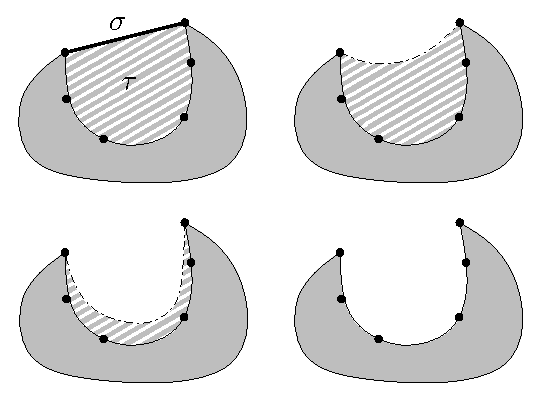
\includegraphics[width=80mm]{img/elementary-collapse.eps}
\caption{Elementarne zgniecenie.}\label{fig-elementary-collapse}
\end{figure}

Nietrudno spostrzec (zob.~rysunek \ref{fig-elementary-collapse}), że jeżeli $X\elcoll Y$, to $Y$~jest mocnym retraktem deformacyjnym $X$; co więcej, jeśli $\mP(Y)=\mP(X)\smallsetminus \{\sigma,\tau\}$, gdzie $\sigma$~jest właściwą ścianą $\tau$, to mocną retrakcję deformacyjną $r\colon X\to Y$ można wybrać w~ten sposób\label{mocna_retr_def_przy_el_zgnieceniu_ze_jest_fajna}, że \[r(\sigma\cup\tau)\subseteq \bigcup\{\rho\in \mP(Y):\rho \text{ jest ścianą } \tau \text{ w } X\}.\] 

Mówimy, że regularne CW kompleksy $X$, $Y$ mają ten sam \textit{prosty typ homotopijny}\index{typ homotopijny!prosty} (lub że są \textit{prosto homotopijnie równoważne}\index{homotopijna rozzzwnowazzzznoszzzczzz@homotopijna równoważność!prosta}), i~piszemy $X\simplehe Y$\nomenclature[7d]{$X\simplehe Y$}{regularne CW kompleksy $X$, $Y$ mają ten sam prosty typ homotopijny}, o~ile istnieje ciąg regularnych CW kompleksów $(X_i)_{i=0}^{n}$ taki, że $X_0=X$, $X_n=Y$ oraz dla każdego indeksu $i=0,\ldots,n-1$ zachodzi jeden z~warunków: $X_{i}\searrow X_{i+1}$ lub $X_{i+1}\searrow X_{i}$. Prosto homotopijnie równoważne CW kompleksy są, wobec obserwacji poczynionych w~poprzednim akapicie, homotopijnie równoważne.

Dobre wprowadzenie do interesującego fragmentu topologii algebraicznej, jaki stanowią zagadnienia związane z~prostym typem homotopijnym, stanowi książka Cohena \cite{Cohen73}.

Ponieważ każdy kompleks symplicjalny można utożsamiać z~pewnym regularnym CW kompleksem, możemy mówić o~prostym typie homotopijnym (oraz zgnieceniach itp.) kompleksów symplicjalnych.

Zdefiniujemy indukcyjnie związaną ze zgniatalnością kompleksów symplicjalnych własność, wywodzącą się z~teorii złożoności \cite{Kahn84}. Mówimy, że skończony kompleks symplicjalny $K$~jest \textit{non-evasive}\index{kompleks symplicjalny!non-evasive@\textit{non-evasive}}, jeśli $K$~składa się z~pojedynczego wierzchołka lub istnieje wierzchołek $v\in K$ taki, że kompleksy symplicjalne $\lk_K(v)$ oraz $K-v$ są \textit{non-evasive}. Jeżeli kompleks symplicjalny ma własność \mbox{\textit{non-evasiveness}}, to jest zgniatalny~\cite{Kahn84}.

\begin{tw}[{\cite[Theorem 2.10]{Welker99}}]\label{tw_welkera_o_zgniatalnosci_podzialu}
Jeśli skończony kompleks symplicjalny $K$~jest zgniatalny, to kompleks symplicjalny $\mK(\mP(K))$ ma własność \textit{non-evasiveness}.
\end{tw}


%====================================================================
%====================================================================
%====================================================================




\begin{comment}

\section{Geometria metryczna}\label{sec-geometria_metryczna}
Niech $(X,d)$ będzie przestrzenią metryczną. Określamy odległość punktu $x\in X$~od zbioru $A\subseteq X$ jako $d(x,A)=\inf\{a\in A:d(x,a)\}$.

\textit{Krzywą geodezyjną} (albo po prostu \textit{geodezyjną}) łączącą punkty $x,y\in X$ nazywamy odwzorowanie ciągłe $c\colon [0,l]\to X$ takie, że $c(0)=x, c(l)=y$ oraz $d(c(t),c(t'))=|t-t'|$ dla wszystkich $t,t'\in [0,l]$. W~szczególności mamy $l=d(x,y)$. \textit{Odcinkiem geodezyjnym} o~końcach $x,y$ nazywamy zbiór $c([0,l])\subseteq X$. Odcinek taki oznaczać będziemy czasem symbolem $[x,y]$. Istnieje wzajemnie jednoznaczna odpowiedniość pomiędzy geodezyjnymi w~$X$~a~parami $(x,\alpha)$, gdzie $\alpha$~jest odcinkiem geodezyjnym w~$X$~o~końcu $x$.

Mówimy, że przestrzeń $(X,d)$ jest \textit{geodezyjna}, jeśli dla każdej pary punktów $x,y\in X$ istnieje krzywa geodezyjna je łącząca. Dla $r>0$ przestrzeń $X$~nazywamy \textit{$r$-geodezyjną}, jeśli dla każdej pary punktów $x,y\in X$ takiej, że $d(x,y)<r$, istnieje geodezyjna je łącząca. 

Podzbiór $C$~geodezyjnej przestrzeni metrycznej $(X,d)$ nazywamy \textit{wypukłym}, jeśli każdą parę punktów $x,y\in C$ można połączyć geodezyjną w~$X$ oraz obraz każdej geodezyjnej łączącej te punkty zawiera się w~zbiorze $C$. \textit{Otoczką wypukłą} podzbioru geodezyjnej przestrzeni metrycznej nazywamy część wspólną wszystkich zbiorów wypukłych zawierających ten podzbiór.

Mówimy, że przestrzeń metryczna $(X,d)$ jest \textit{właściwa}, jeśli dla każdego $r\geq 0$ i~każdego $x\in X$ kula domknięta $D(x,r)=\{y\in X:d(x,y)\leq r\}$ jest zbiorem zwartym w~$X$. Przypomnijmy, że przestrzeń $(X,d)$ nazywamy \textit{zupełną}, gdy każdy ciąg Cauchy'ego w~$X$~jest zbieżny.

\textit{Średnicą} podzbioru $A\subseteq X$ przestrzeni metrycznej $(X,d)$ nazywamy liczbę $\operatorname{diam}(A)=\sup\{d(x,y):x,y\in A\}$.\nomenclature[ozn_srednica]{$\operatorname{diam}(A)$}{średnica zbioru $A$}

Dla $x,y\in\mR^n$ niech \[\langle x,y\rangle=\sum_{i=0}^{n-1}x_i y_i,\quad \langle\!\langle x,y\rangle\!\rangle=-x_{n-1}y_{n-1}+\sum_{i=0}^{n-2}x_i y_i\] oraz niech $\|x\|=\sqrt{\langle x, x\rangle}$

Zdefiniujemy dla $\kappa\in \mR$ oraz $n\in\mN$, $n\geq 1$ tzw.~\textit{przestrzenie modelowe} $M_\kappa^n$. Jeśli $\kappa>0$, to za $M_\kappa^n$ przyjmujemy sferę $\S^n$ z~metryką \[d(x,y)=\frac{1}{\sqrt{\kappa}} \operatorname{arccos}\left(\langle x,y\rangle\right)=\frac{2}{\sqrt{\kappa}} \operatorname{arcsin}\left(\frac{\|x-y\|}{2}\right).\]
Jeżeli $\kappa=0$, to $M^n_\kappa=\mathbb{R}^n$ z~metryką zadaną przez normę $\|\cdot\|$. Jeśli natomiast $\kappa<0$, to definiujemy $M^n_\kappa$ jako zbiór \[\mathbf{H}^n=\{x\in \mR^{n+1}:\langle\!\langle x,x\rangle\!\rangle=-1, x_{n}>0\}\] z~metryką zadaną dla $x,y\in \mathbf{H}^n$ wzorem \[d(x,y)=\frac{1}{\sqrt{-\kappa}}\operatorname{arccosh} (-\langle\!\langle x,y\rangle\!\rangle).\] 
\textit{Trójkątem geodezyjnym} $\Delta([x,y],[y,z],[z,x])$ w~przestrzeni metrycznej $(X,d)$ nazywamy układ trzech punktów $x,y,z\in X$ oraz łączących je odcinków geodezyjnych $[x,y], [y,z], [z,x]\subseteq X$. \textit{Trójkątem porównawczym} dla danego trójkąta geodezyjnego $\Delta([x,y],[y,z],[z,x])$ w~przestrzeni modelowej $M^2_\kappa$ nazywamy taki trójkąt geodezyjny $\Delta([\bar{x},\bar{y}],[\bar{y},\bar{z}],[\bar{z},\bar{x}])$ w~przestrzeni $M^2_\kappa$, że $d(x,y)=d(\bar{x},\bar{y})$, $d(y,z)=d(\bar{y},\bar{z})$, $d(z,x)=d(\bar{z},\bar{x})$. Trójkąt taki istnieje, o~ile zachodzi następująca nierówność dla długości obwodu tego trójkąta \[d(x,y)+d(y,z)+d(x,z)<2\operatorname{diam}(M^2_\kappa)=\begin{cases}\frac{2\pi}{\sqrt{\kappa}} & \text{dla } \kappa>0,\\\infty & \text{dla } \kappa\leq 0.\end{cases}\] Dla $p\in [x,y]$ \textit{punktem porównwawczym} w~trójkącie porównawczym $\Delta([\bar{x},\bar{y}],[\bar{y},\bar{z}],[\bar{z},\bar{x}])$ nazywamy taki element $\bar{p}\in [\bar{x},\bar{y}]$, że $d(x,p)=d(\bar{x},\bar{p})$; podobnie definiujemy punkty porównwacze dla elementów odcinków $[y,z],[z,x]$. Mówimy, że trójkąt geodezyjny $\Delta([x,y],[y,z],[z,x])$ spełnia \textit{nierówność $\CAT(\kappa)$}, jeśli długość obwodu tego trójkąta jest mniejsza niż $2\operatorname{diam}(M^2_\kappa)$ oraz dla wszystkich punktów $p,q\in [x,y]\cup [y,z]\cup [z,x]$ zachodzi nierówność $d(p,q)\leq d(\bar{p},\bar{q})$, gdzie $\bar{p},\bar{q}$ są punktami porównawczymi dla $p,q$ należącymi do trójkąta porównawczego dla trójkąta $\Delta([x,y],[y,z],[z,x])$ w~przestrzeni $M^2_\kappa$.

Jeśli $\kappa\leq 0$, to przestrzeń metryczną $X$~nazywamy \textit{przestrzenią $\CAT(\kappa)$}, jeżeli jest przestrzenią geodezyjną i~wszystkie trójkąty geodezyjne w~$X$~spełniają nierówność $\CAT(\kappa)$. Jeśli natomiast $\kappa>0$, to $X$~nazywamy \textit{przestrzenią $\CAT(\kappa)$}, gdy $X$~jest przestrzenią $\operatorname{diam}(M^2_\kappa)$-geodezyjną oraz wszystkie trójkąty geodezyjne w~$M^2_\kappa$ o~długości obwodu mniejszej niż $2\operatorname{diam}(M^2_\kappa)$ spełniają nierówność $\CAT(\kappa)$. Nazwa ,,$\CAT(\kappa)$'' została zaproponowana przez Gromova \cite{Gromov87} i~pochodzi od nazwisk E.~Cartana, A.D.~Aleksandrowa oraz V.A.~Toponogova. 

\begin{stw}[{\cite[Proposition II.1.4]{Bridson99}}]
Jeżeli $X$~jest przestrzenią $\CAT(\kappa)$, gdzie $\kappa\leq 0$ lub $\kappa>0$ oraz $\operatorname{diam}(X)<\frac{\pi}{\sqrt{\kappa}}$, to przestrzeń $X$~jest ściągalna.
\end{stw}

\begin{lem}[{\cite[Proposition II.2.4, Exercise II.2.6(1)] {Bridson99}}]\label{lemat-bridsona-o-jedynym-punkcie}
Niech $X$~będzie spójną przestrzenią $\CAT(\kappa)$, $x\in X$ jej elementem, zaś $C\subseteq X$ wypukłym, zupełnym podzbiorem. Jeżeli $\kappa\leq 0$ lub $\kappa\geq 0$ oraz $d(x,C)<\frac{\pi}{2\sqrt{\kappa}}$, to istnieje dokładnie jeden element $c\in C$ taki, że $d(x,c)=d(x,C)$.
\end{lem}

Niech $n\leq m$ będą dodatnimi liczbami naturalnymi oraz niech $\kappa\in\mathbb{R}$. \textit{Geodezyjnym $n$-wymiarowym sympleksem w~przestrzeni $M^m_\kappa$} nazywamy zbiór $S\subseteq M^m_\kappa$ będący otoczką wypukłą $n+1$ punktów $\{v_0,\ldots,v_n\}$ należących do $M^m_\kappa$ i~znajdujących się w~położeniu ogólnym, tzn.~nie zawierających się w~żadnej podprzestrzeni $M^m_\kappa$ izometrycznej z~$M^{n-1}_\kappa$, przy czym jeśli $\kappa>0$, to wymagamy dodatkowo, aby zbiór $\{v_0,\ldots,v_n\}$ zawierał się w~otwartej półsferze sfery $M^{m}_\kappa$. Elementy $v_0,\ldots,v_n\in M^m_\kappa$ nazywamy \textit{wierzchołkami} geodezyjnego sympleksu~$S$. Dla każdego punktu $s\in S$ określimy jego \textit{współrzędne barycentryczne} $b_0(s),\ldots,b_n(s)\in \I$. Jeżeli $\kappa=0$, to wierzchołki $v_0,\ldots,v_m$ są wektorami przestrzeni $M^m_\kappa=\mathbb{R}^{m}$. Współrzędne barycentryczne punktu $s$~określamy w~tym przypadku jako jedyne liczby z~odcinka jednostkowego $\I$ spełniające warunek \[x=b_0(s) v_0+\ldots+b_n(s) v_n.\] Jeśli $\kappa>0$, to $M^m_\kappa=\S^{m}\subseteq \mathbb{R}^{m+1}$. Otoczka wypukła wierzchołków $v_0,\ldots,v_n$ jest sympleksem $S'$ w~$\mathbb{R}^{m+1}$. Ponadto $0\not\in S'$, ponieważ wierzchołki te zawierają się w~otwartej półsferze sfery $\S^m$. Odwzorowanie $p\colon S\to S'$ zadane dla $x\in S'$ wzorem $p(x)=\frac{x}{\|x\|}$ jest bijekcją. Jako współrzędne barycentryczne punktu $s$~przyjmujemy współrzędne barycentryczne punktu $p^{-1}(s)$ w~sympleksie $S'$. Podobnie postępujemy dla $\kappa<0$. Współrzędne barycentryczne wyznaczają element $s\in S$ w~sposób jednoznaczny; możemy zatem $s$~utożsamiać z~funkcją $\tilde{s}\colon \{v_0,\ldots,v_n\}\to \I$ taką, że $\tilde{s}(v_i)=b_i(s)$.

Jeżeli $S, S'$ są $n$-wymiarowymi sympleksami geodezyjnymi odpowiednio w~$M^m_\kappa$ oraz $M^{m'}_{\kappa'}$, o~zbiorach wierzchołków $\{v_0,\ldots,v_n\}$ oraz $\{v_0',\ldots,v_{n}'\}$, to istnieje dokładnie jedno odwzorowanie $S\to S'$ zachowujące współrzędne barycentryczne i~przeprowadzające $v_i$ na $v_i'$ dla wszystkich $i=1,\ldots,n$. Podobnie, $\sigma\in K$ jest \mbox{$n$-wymiarowym} sympleksem kompleksu symplicjalnego $K$, $\sigma=\{v_0'',\ldots,v_n''\}$, to istnieje dokładnie jedno odwzorowanie $f\colon S\to |\sigma|$ z~sympleksu $S$~w~domknięty sympleks $|\sigma|\subseteq |K|$ takie, że $f(s)(v_i'')=\tilde{s}(v_i)$ dla $s\in S$ oraz wszystkich $i=1,\ldots,n$. Odwzorowania te, zwane \textit{afinicznymi}, są homeomorfizmami.

Kompleksem $M_\kappa$-symplicjalnym nazywamy trójkę \[\mathbb{K}=\left(K,\ \Shapes(\mathbb{K}),\ \{f_\sigma\colon S_\sigma\to |\sigma|\}_{\sigma\in K}\right),\] gdzie $K$~jest kompleksem symplicjalnym, $\Shapes(\mathbb{K})$ pewnym zbiorem geodezyjnych sympleksów w~przestrzeniach $M^{n}_\kappa$, $n\in\mN$, dla każdego sympleksu $\sigma$~istnieje geodezyjny, $\dim(\sigma)$-wymiarowy sympleks $S_\sigma\in \Shapes(\mathbb{K})$, a~$f_\sigma\colon S_\sigma\to |\sigma|$~jest afinicznym homeomorfizmem tego sympleksu na domknięty sympleks $|\sigma|\subseteq |K|$, przy czym jeżeli $\sigma,\tau\in K$ oraz $\sigma\subseteq \tau$, to odwzorowanie $f_\tau^{-1}\circ f_\sigma\colon S_\sigma \to S_\tau$ jest izometrią na obraz.

\textit{Nicią} w~kompleksie $M_\kappa$-symplicjalnym pomiędzy elementami $x,y\in |K|$ nazywamy ciąg $\Sigma=(x=x_0,x_1,\ldots,x_{n(\Sigma)}=y)$ elementów $K$~o~tej własności, że dla każdego $i=0,\ldots,n(\Sigma)-1$ istnieje sympleks $\sigma_i\in K$ taki, że $x_i,x_{i+1}\in |\sigma|$. \textit{Długością} nici $\Sigma$ nazywamy liczbę \[l(\Sigma)=\sum_{i=0}^{n(\Sigma)-1}d_{S_{\sigma_i}}\left(f_{\sigma_i}^{-1}(x_i),f_{\sigma_i}^{-1}(x_{i+1})\right),\]
gdzie $d_{S_{\sigma_i}}\colon S_{\sigma_i}\times S_{\sigma_i}\to \mathbb{R}$ jest funkcją odległości w~sympleksie $S_{\sigma_i}$. Jeśli kompleks symplicjalny $K$~jest spójny, określić można pewną funkcję $d_\mathbb{K}\colon |K|\times |K|\to \mathbb{R}$, dla $x,y\in |K|$ zadaną wzorem
\[d_\mathbb{K}(x,y)=\inf\{l(\Sigma): \Sigma\text{ jest nicią z } x \text{ do } y\}.\]
Na ogół tak zdefiniowana funkcja $d_\mathbb{K}$~nie jest metryką na $|K|$.

\begin{tw}[Bridsona, {\cite[Theorem I.7.19, Exercise I.7.62]{Bridson99}}]\label{tw-bridsona}
Jeżeli $\mathbb{K}=\left(K,\ \Shapes(\mathbb{K}),\ \{f_\sigma\}_{\sigma\in K}\right)$ jest kompleksem $M_\kappa$-symplicjalnym takim, że kompleks symplicjalny $K$~jest spójny oraz dla wszystkich $x\in |K|$ oraz $n\in \mN$ zbiór \[\bigl\{S_\sigma\in \Shapes(K):\sigma\in K,\ |\sigma|\subseteq \{y\in |K|: d_K(x,y)\leq n\}\bigr\}\] jest skończony, to  $(|K|,d_\mathbb{K})$ jest zupełną przestrzenią geodezyjną.
% oraz zbiór $\Shapes(K)$~jest skończony, to $(|K|,d_\mathbb{K})$ jest zupełną przestrzenią geodezyjną.

% Teza twierdzenia zachodzi również przy słabszym założeniu, że dla wszystkich $x\in |K|$ oraz $n\in \mN$ zbiór \[\bigl\{S_\sigma\in \Shapes(K):\sigma\in K,\ |\sigma|\subseteq \{y\in |K|: d_K(x,y)\leq n\}\bigr\}\] jest skończony.
\end{tw}

Kompleks $M_0$-symplicjalny $\mathbb{K}$~nazywamy \textit{regularnym}, o~ile długość wszystkich krawędzi każdego sympleksu $S\in\Shapes(\mathbb{K})$ wynosi $1$.

\end{comment}

%====================================================================
%====================================================================
%====================================================================





\section{Topologia w nieskończoności}\label{sec-top_w_nsk}
\textbf{Do końca podrozdziału \ref{sec-top_w_nsk} zakładamy, że $X$, $Y$~są przestrzeniami topologicznymi będącymi sumami rozłącznymi skończonej liczby uogólnionych continuów.} 

Podrozdział opiera się w~dużej mierze na książkach Bauesa i~Quintero~\cite{Baues01} oraz Hughesa i~Ranickiego \cite{Hughes96}.

\subsection{Właściwy typ homotopijny}
Jeżeli $f,g\colon X\to Y$ są właściwymi odwzorowaniami, to mówimy, że odwzorowania te są \textit{homotopijne w~sposób właściwy}, co oznaczamy przez $f\overset{p}{\simeq} g$\nomenclature[1m]{$f \overset{p}{\simeq} g$}{właściwe odwzorowania $f, g$ są homotopijne w~sposób właściwy}, jeżeli istnieje homotopia $H\colon X\times \I\to Y$ pomiędzy $f$ oraz~$g$ będąca właściwym odwzorowaniem (tzn.~\textit{właściwa homotopia}). Przestrzenie $X,Y$ nazywamy \textit{homotopijnie równoważnymi w~sposób właściwy}, jeżeli istnieje \textit{właściwa homotopijna równoważność}\index{homotopijna rozzzwnowazzzznoszzzczzz@homotopijna równoważność!wlzzzaszzzciwa@właściwa}\index{typ homotopijny!wlzzzaszzzciwy@właściwy} $X\to Y$, to znaczy takie właściwe odwzorowanie $f\colon X\to Y$, że dla pewnego właściwego odwzorowania $g\colon Y\to X$ istnieją właściwe homotopie $f\circ g\overset{p}{\simeq}\id_Y$ oraz~$g\circ f\overset{p}{\simeq}\id_X$.

Mówimy, że przestrzeń $X$~będąca ANR-em jest \textit{ściągalna w~sposób właściwy}\index{szzzciazzzgalnoszzzczzz w~sposozzzb wlzzzaszzzciwy@ściągalność w~sposób właściwy}\index{ANR!szzzciazzzgalny w~sposozzzb wlzzzaszzzciwy@ściągalny w~sposób właściwy}\index{przestrzenzzz topologiczna@przestrzeń topologiczna!szzzciazzzgalna w~sposozzzb wlzzzaszzzciwy@ściągalna w~sposób właściwy}, jeżeli przestrzeń $X$~jest homotopijnie równoważna w~sposób właściwy realizacji geometrycznej $1$-wymiarowego, lokalnie skończonego, spójnego i~acyklicznego kompleksu symplicjalnego (czyli drzewa).

\subsection{Zbiór końców}
Przez \textit{koniec}\index{koniec!przestrzeni topologicznej} przestrzeni $X$~rozumiemy odwzorowanie \[\varepsilon\colon \{K\subseteq X:K\text{ jest zwarty}\}\to 2^X\smallsetminus \{\emptyset\}\] takie, że dla wszystkich zbiorów zwartych $K,L\subseteq X$ spełnione są poniższe dwa warunki:
\begin{compactenum}
\item zbiór $\varepsilon(K)$ jest składową spójności przestrzeni $X\smallsetminus K$;
\item jeżeli $L\subseteq K$, to $\varepsilon(K)\subseteq \varepsilon(L)$.
\end{compactenum}
Symbolem $\E(X)$ oznaczamy zbiór wszystkich końców przestrzeni $X$\index{zbiozzzr@zbiór!konzzzcozzzw@końców!przestrzeni topologicznej}.
Podana definicja końca przestrzeni topologicznej pochodzi z~pracy Milnora \cite{Milnor68} i~dla uogólnionych continuów jest równoważna innym znanym definicjom końca (por.~\cite[Chapter~1]{Hughes96}).

\begin{ex}\noindent
\begin{compactenum}
\item Uogólnione continuum $X$~jest zwartą przestrzenią topologiczną wtedy i~tylko wtedy, gdy $\E(X)=\emptyset$.
\item Prosta rzeczywista $\mR$ ma dokładnie dwa końce, natomiast każda z przestrzeni $\mR^n$ dla $n\geq 2$ ma dokładnie jeden koniec.
\item Dla każdej liczby $n\in\mN$ przestrzeń \[X_n=\bigl( [0,\infty)\times \{0\} \bigr) \cup \bigl(\{0,\ldots,n-1\}\times [0,\infty)\bigr)\subseteq \mathbb{R}^2\] z~topologią indukowaną z~płaszczyzny $\mathbb{R}^2$ ma dokładnie $n+1$~końców. Ponadto zbiór końców przestrzeni $\bigcup_{n\in\mN} X_n$ jest przeliczalnie nieskończony.
\item Zbiór końców nakrycia uniwersalnego bukietu dwóch okręgów jest nieprzeliczalny.
\end{compactenum}
\end{ex}

Dla właściwego odwzorowania $f\colon X\to Y$ określimy indukowaną przez nie funkcję $\E(f)\colon \E(X)\to \E(Y)$. Jeżeli $\varepsilon\in \E(X)$ oraz $K\subseteq Y$ jest zbiorem zwartym, przyjmujemy za $\E(f)(\varepsilon)(K)$ tę spójną składową przestrzeni $Y\smallsetminus K$, dla której \[f\left(\varepsilon\left(f^{-1}(K)\right)\right)\subseteq \E(f)(\varepsilon)(K).\] Nietrudno zauważyć, że taka spójna składowa istnieje i~jest tylko jedna \cite[Proposition 1.22]{Hughes96}; ponadto $\E(f)(\varepsilon)\in \E(Y)$. Funkcja $\E(f)\colon \E(X)\to \E(Y)$ jest więc dobrze określona. Co więcej, łatwo sprawdza się, iż przyporządkowanie $\E$\nomenclature[6a]{$\E$}{funktor zbioru końców przestrzeni topologicznej (lub częściowego porządku)} jest funktorem z~kategorii przestrzeni topologicznych będących sumami rozłącznymi skończonej liczby uogólnionych continuów oraz ich właściwych odwzorowań w~kategorię zbiorów i~funkcji, oraz że jeśli właściwe odwzorowania $f,g\colon X\to Y$ są homotopijne w~sposób właściwy, to $\E(f)=\E(g)$ (zob.~\cite[Proposition 1.22]{Hughes96}).

Następujący lemat stanowi prosty wniosek z~lematu \ref{lem-sigma_zwarta_kazdy_zwarty_w_wyczerpujacym}.
\begin{lem}\label{lem-co_wyznacza_koniec_w_sigma_zwartej}
Załóżmy, że $(C_i)_{i\in\mN}$ jest ciągiem wyczerpującym przestrzeń $X$. Niech $Z$~oznacza zbiór funkcji $\delta\colon \{C_i\}_{i\in\mN}\to 2^X\smallsetminus \{\emptyset\}$ takich, że dla każdego $i\in\mN$ zbiór $\delta(C_i)$~jest nieograniczoną składową spójności przestrzeni $X\smallsetminus C_i$ oraz $\delta(C_j)\subseteq \delta(C_i)$ dla $j\geq i$. Funkcja $\E(X)\to Z$ przyporządkowująca końcowi $\varepsilon\in \E(X)$ jego ograniczenie $\varepsilon\big |_{\{C_i\}_{i\in\mN}}$ jest bijekcją.
\end{lem}

\begin{lem}\label{lem-istnieje_koniec_w_strone_danej_skladowej}
Niech $K$~będzie zwartym podzbiorem $X$, zaś~$S$ nieograniczoną w~$X$~składową spójności zbioru $X\smallsetminus K$. Istnieje wówczas koniec $\varepsilon\in\E(X)$ taki, że $\varepsilon(K)=S$.
\end{lem}
\begin{proof}
Na podstawie lematu \ref{lem-istnieje_ciag_wyczerpujacy} istnieje wyczerpujący przestrzeń $X$~ciąg $(C_i)_{i\in\mN}$ taki, że $C_0=K$. Określimy pewną funkcję $\delta\colon \{C_i\}_{i\in \mN}\to 2^X\smallsetminus\{\emptyset\}$. Niech $\delta(C_0)=S$. Ustalmy $n>0$ i~załóżmy, że dla wszystkich liczb naturalnych $i<n$ określone są zbiory $\delta(C_i)\in 2^X\smallsetminus\{\emptyset\}$, przy czym $\delta(C_i)$ jest nieograniczoną składową spójności $X\smallsetminus C_i$ oraz $\delta(C_j)\subseteq \delta(C_i)$ dla wszystkich $i\leq j<n$. Za $\delta(C_{n})$ przyjmujemy dowolną nieograniczoną składową spójności zbioru $X\smallsetminus C_{n}$ zawartą w~$\delta(C_{n-1})$.

Wobec lematu \ref{lem-co_wyznacza_koniec_w_sigma_zwartej} istnieje koniec $\varepsilon\in \E(X)$ taki, że $\varepsilon\big|_{\{C_i\}_{i\in\mN}}=\delta$. W~szczególności $\varepsilon(K)=\delta(K)=S$.
\end{proof}



%--------------------------------------------------------------------
%-------------------------------------------------------------------
%-------------------------------------------------------------------


\subsection{Uzwarcenie Freudenthala}
Dla końca $\varepsilon\in \E(X)$ oraz zwartego zbioru $K\subseteq X$ przyjmijmy oznaczenia \begin{align*}B(\varepsilon,K)&=\{\varepsilon'\in \E(X): \varepsilon(K)=\varepsilon'(K)\},\\N(\varepsilon,K)&=\varepsilon(K)\cup B(\varepsilon,K).\end{align*} 

\textit{Uzwarceniem Freudenthala}\index{uzwarcenie!Freudenthala} \cite{Freudenthal31, Raymond60} przestrzeni $X$~nazywamy przestrzeń $\F X=X\cup \E(X)$ z~topologią zadaną przez następujące bazy otoczeń otwartych: dla $x\in X$ jako bazę otoczeń otwartych przyjmujemy dowolną bazę otoczeń otwartych tego punktu w~przestrzeni $X$, natomiast dla końca $\varepsilon\in\E(X)$ bazą otoczeń otwartych jest rodzina $\{N(\varepsilon,K): K\subseteq X\text{ jest zbiorem zwartym}\}$.

Niech $f\colon X\to Y$ będzie właściwym odwzorowaniem. Określmy funkcję $\F f\colon \F X\to \F Y$ dla elementu $a\in \F X$ przyjmując \[\F f(a)=\begin{cases}f(a), &\text{jeżeli } a\in X,\\ \E(f)(a), & \text{jeżeli } a\in\E(X).\end{cases}\]

\begin{stw}[{\cite[Proposition I.9.11]{Baues01}}]\label{stw-funkcja_freudenthala_ciagla}
Jeśli $f\colon X\to Y$ jest właściwym odwzorowaniem, to funkcja $\F f\colon \F X\to \F Y$ jest ciągła.
\end{stw}

Wobec stwierdzenia \ref{stw-funkcja_freudenthala_ciagla} przyporządkowanie $\F$ jest  funktorem\nomenclature[6b]{$\F$}{funktor uzwarcenia Freudenthala} z~kategorii przestrzeni topologicznych będących sumami rozłącznymi skończonej liczby uogólnionych continuuów i~ich właściwych odwzorowań w~kategorię przestrzeni topologicznych i~funkcji ciągłych.

\begin{comment}
Uzwarcenie Freudenthala można scharakteryzować w~następujący sposób.

\begin{tw}[\cite{Raymond60}]\label{tw-raymonda}
Niech $X^*$ będzie uzwarceniem przestrzeni $X$ o~następujących własnościach:
\begin{compactenum}
\item przestrzeń $X^*$ jest spójna;
\item $X$ jest otwartym podzbiorem $X^*$;
\item przestrzeń $X^*\smallsetminus X$ jest całkowicie niespójna;
\item jeśli $p\in X^*\smallsetminus X$ oraz $U$~jest spójnym otoczeniem otwartym punktu $p$, to zbiór $U\smallsetminus (X^*\smallsetminus X)$ jest spójny.
\end{compactenum}
Wówczas uzwarcenie $X^*$ jest izomorficzne z~uzwarceniem Freudenthala $\F X$.
\end{tw}
\end{comment}

\begin{lem}[{\cite[Addendum I.9.9]{Baues01}}]\label{lem-uzwarcenie_jest_metryczne}
Jeżeli $X$~jest uogólnionym continuum, to $\F X$~jest continuum. Jeśli $X$~jest uogólnionym continuum Peano, to $\F X$~jest continuum Peano.
\end{lem}

\begin{comment}
\begin{lem}\label{lem-iloraz_homeomorficzny_jednopunktowemu}
Jeśli przestrzeń $X$~jest niezwarta, to przestrzeń ilorazowa $\F X\big/\E(X)$ jest homeomorficzna $X^\infty$.
\end{lem}
\begin{proof}
Ustalmy niezwartą przestrzeń $X$~będącą sumą rozłączną skończonej liczby uogólnionych continuów. Rozważmy funkcję $f\colon \F X\to X^\infty$ zadaną dla $a\in \F X$ wzorem \[f(a)=\begin{cases} a, & \text{jeżeli } a\in X,\\ \infty^X, &\text{jeżeli } a\in \E(X).\end{cases}\]

Oczywiście $\E(X)\not=\emptyset$, więc $f$~jest surjekcją. Jeżeli $U=\bigl\{\infty^X\bigr\}\cup (X\smallsetminus K)$ dla pewnego zbioru zwartego $K\subseteq X$, to \[f^{-1}(U)=(X\smallsetminus K)\cup \E(X)=(X\smallsetminus K)\cup \bigcup_{\varepsilon\in \E(X)}N(\varepsilon,K)\] jest zbiorem otwartym w~$\F X$. Wobec przyjętej definicji topologii na przestrzeni $X^\infty$ przekształcenie $f$~jest więc ciągłe. Wykażemy, że $f$~jest odwzorowaniem ilorazowym, tzn.~że topologia na $X^\infty$ jest najbogatszą spośród topologii na tym zbiorze, przy których funkcja $f$~jest ciągła, co będzie oznaczało, że $X^\infty\approx \F X\big/\E(X)$.

Rozważmy w~tym celu taki podzbiór $U\subseteq X^\infty$, że zbiór $f^{-1}(U)\subseteq \F X$ jest otwarty. Jeżeli $\infty^X\not\in U$, to $f^{-1}(U)=U\subseteq X$ jest zbiorem otwartym w~$X$, a~zatem również w~$X^\infty$. Jeśli natomiast $\infty^X\in U$, to $\E(X)\subseteq f^{-1}(U)$. Możemy więc przedstawić zbiór $f^{-1}(U)$ jako sumę \[f^{-1}(U)=V\cup \bigcup_{\varepsilon\in \E(X)}\bigcup_{K\in \mathfrak{K}(\varepsilon)} N(\varepsilon, K),\] gdzie $V$~jest otwartym podzbiorem $X$, zaś $\mathfrak{K}(\varepsilon)\subseteq 2^{X}$ jest, dla każdego końca $\varepsilon\in\E(X)$, pewną rodziną zwartych podzbiorów przestrzeni $X$. Ponieważ $X$~jest otwartym podzbiorem zwartej przestrzeni $\F X $, zbiór $\E(X)=\F X\smallsetminus X$ jest zwarty. Rodzina \[\left\{N(\varepsilon,K):\varepsilon\in\E(X), K\in\mathfrak{K}(\varepsilon)\right\}\] jest otwartym pokryciem $\E(X)$. Można zatem wybrać końce $\varepsilon_1,\ldots, \varepsilon_n\in \E(X)$ oraz zbiory zwarte $K_i\in\mathfrak{K}(\varepsilon_i)$, $i=1,\ldots, n$, o~tej własności, że skończona rodzina $\{N(\varepsilon_i,K_{i})\}_{i=1}^{n}$ jest otwartym pokryciem zbioru $\E(X)$. W~szczególności, dla każdego końca $\delta\in \E(X)$ istnieje indeks $i_\delta\in \{1,\ldots, n\}$ taki, że $\delta\in N\left(\varepsilon_{i_\delta},K_{i_\delta}\right)$, to znaczy $\delta\left(K_{i_\delta}\right)=\varepsilon_{i_\delta}\left(K_{i_\delta}\right)$. Zbiór $\bigcup_{i=1}^{n}K_i\subseteq X$ jest zwarty jako skończona suma zbiorów zwartych. Na podstawie lematu \ref{lem-dorzucanie_skladowych_a_zwartosc} istnieje zwarty podzbiór $\hat{K}\subseteq X$ zawierający $\bigcup_{i=1}^{n}K_i$ oraz~taki, że każda składowa spójności zbioru $X\smallsetminus \hat{K}$ jest nieograniczona w~$X$. Dla dowolnego końca $\delta\in \E(X)$ mamy \[\delta\left(\hat{K}\right)\subseteq \delta\left(K_{i_\delta}\right)=\varepsilon_{i_\delta}\left(K_{i_\delta}\right)\subseteq B\left(\varepsilon_{i_\delta},K_{i_\delta}\right)\subseteq U.\] Ponadto, na podstawie lematu \ref{lem-istnieje_koniec_w_strone_danej_skladowej} każda składowa spójności zbioru $X\smallsetminus \hat{K}$ jest postaci $\delta\left(\hat{K}\right)$ dla pewnego końca $\delta\in \E(X)$. Wobec tego $X\smallsetminus \hat{K}\subseteq U$. Zbiór $f^{-1}(U)$ możemy  przedstawić jako poniższą sumę:
\[f^{-1}(U)=V\cup \left(\left(X\smallsetminus \hat{K}\right)\cup \E(X)\right)\cup \bigcup_{\varepsilon\in \E(X)}\bigcup_{K\in \mathfrak{K}(\varepsilon)} \varepsilon(K).\]
Ale zbiór \[V\cup \bigcup_{\varepsilon\in \E(X)}\bigcup_{K\in \mathfrak{K}(\varepsilon)} \varepsilon(K)\] jest otwarty w~$X$. Wobec tego \[U=\left(V\cup \bigcup_{\varepsilon\in \E(X)}\bigcup_{K\in \mathfrak{K}(\varepsilon)} \varepsilon(K)\right)\cup \left(\left(X\smallsetminus \hat{K}\right)\cup \left\{\infty^X\right\}\right)\] jest otwartym podzbiorem $X^\infty$, co kończy dowód lematu.
\end{proof}
\end{comment}




%--------------------------------------------------------------------
%-------------------------------------------------------------------
%-------------------------------------------------------------------



\subsection{Oswojoność}
Przestrzeń $X$ nazywamy \textit{oswojoną na zewnątrz}\footnote{ang. \textit{outward tame}}\index{przestrzenzzz topologiczna@przestrzeń topologiczna!oswojona na zewnazzztrz@oswojona na zewnątrz} \cite{Quinn88,Hughes96}, jeżeli istnieje domknięty, koograniczony podzbiór $V\subseteq X$ taki, że włożenie $V\times \{0\}\hookrightarrow X$ (dla $v\in V$ zadane wzorem $(v,0)\mapsto v$) rozszerza się do właściwego odwzorowania $V\times [0,\infty)\to X$.

Mówimy, że przestrzeń $X$~\textit{ma kołnierzyk na zewnątrz}\footnote{ang. \textit{is outward collared}} \cite{Hughes96}\index{przestrzenzzz topologiczna@przestrzeń topologiczna!ma kolzzznierzyk na zewnazzztrz@ma kołnierzyk na zewnątrz}, jeżeli istnieje domknięty, koograniczony podzbiór $V\subseteq X$ będący ANR-em i~taki, że włożenie $V\times\{0\}\hookrightarrow V$ rozszerza się do właściwego odwzorowania $V\times [0,\infty)\to V$. (Oczywiście każda przestrzeń z~kołnierzykiem na zewnątrz jest oswojona na zewnątrz.)

\begin{comment}
\begin{tw}[{\cite[Proposition 7.2]{Hughes96}}]\label{tw-kolnierzyk_na_zewnatrz_a_brzeg_waldhausena}
Niech $X$~będzie przestrzenią z~kołnierzykiem na zewnątrz oraz niech podzbiór $V\subseteq X$ ma własności jak w~powyższej definicji. Istnieją wówczas homotopijne równoważności $e(X)\simeq e(V)\simeq V$.
\end{tw}
\end{comment}


\begin{ex}[{\cite[Example 7.3]{Hughes96}}]\noindent
\begin{compactenum}
\item Niech $M$~będzie zwartą rozmaitością z~brzegiem $\partial M$. Wówczas przestrzeń $X=M\smallsetminus \partial M$ ma kołnierzyk na zewnątrz. % oraz $e(X)\simeq \partial M$.
\item Niech $\left(f_j\colon X_j\to X_{j+1}\right)_{j\in\mN}$ będzie systemem prostym przekształceń pomiędzy zwartymi ANR-ami. \textit{Teleskopem} tego systemu nazywamy przestrzeń \[\operatorname{Tel}\left(f_j\right)_{j\in\mN}=\left(\coprod_{j=0}^{\infty} (X_j\times \I)\right)\big/\sim\ ,\] gdzie $\sim$~jest najmniejszą relacją równoważności na zbiorze $\coprod_{j=0}^\infty (X_j\times \I)$ taką, że $(x_j,1)\sim (f_j(x_j),0)$ dla wszystkich $x_j\in X_j$, $j\in\mN$. Teleskop $\operatorname{Tel}\left(f_j\right)_{j\in\mN}$ ma kołnierzyk na zewnątrz.
\item Niech $X$~będzie przestrzenią topologiczną, $A\subseteq X$ jej podzbiorem, $U\subseteq X$ otoczeniem $A$ oraz niech $V\subseteq U$. Mówimy, że zbiór~$V$~jest \textit{I-kompresowalny} w~$U$ w~kierunku $A$, jeżeli dla każdego otoczenia $W\subseteq X$ zbioru $A$~istnieje izotopia $(h_t)_{t\in \I}$ taka, że \[h_0=\id_X,\quad h_1(V)\subseteq W, \quad h_t\big|_{Z\cup X\smallsetminus U}=\id_{Z\cup X\smallsetminus U}\] dla pewnego otoczenia $Z$~zbioru $A$~oraz wszystkich $t\in \I$. Jeśli dla każdego otoczenia $U$~zbioru $A\subseteq X$ istnieje otoczenie $V\subseteq U$~tego zbioru o~tej własności, że $V$~jest I-kompresowalne w~$U$~w~kierunku $A$, to mówimy, że $A$~ma \textit{otoczenie I-regularne} w~$X$ (zob. \cite{Siebenmann73}).

Niech $A$~będzie zwartym podzbiorem wnętrza zwartej rozmaitości $M$. Jeśli $A$~ma I-regularne otoczenie w~$M$, to przestrzeń $M\smallsetminus A$ jest oswojona na zewnątrz. Jest tak w~szczególności, gdy przestrzeń $A$~ma typ homotopijny (czy ogólniej kształt) CW kompleksu i~jest 1-LCC zanurzona w~$M$ (tzn.~dla każdego $a\in A$ i~otwartego otoczenia $U$~tego punktu w~$M$ istnieje otoczenie otwarte $a\in V\subseteq U$ takie, że każde ciągłe przekształcenie $\S^1\to V\smallsetminus A$ rozszerza się do ciągłego odwzorowania $\D^2\to U\smallsetminus A$).
\item Więcej przykładów przestrzeni oswojonych na zewnątrz odnaleźć można w~książce Hughesa i~Ranickiego \cite{Hughes96}.
\end{compactenum}
\end{ex}

Przestrzeń $X$~nazywamy \textit{oswojoną do wewnątrz}\index{przestrzenzzz topologiczna@przestrzeń topologiczna!oswojona do wewnazzztrz@oswojona do wewnątrz}\footnote{ang. \textit{inward tame}}\label{def-osw_do_wew} \cite{Chapman76,Hughes96}, o~ile dla każdego koograniczonego podzbioru $U\subseteq X$ istnieją koograniczony w~$X$~podzbiór $V\subseteq U$ oraz homotopia $h\colon X\times \I\to X$ o~następujących własnościach:
\begin{compactitem}
\item[---] $h_0=\id_X$;
\item[---] $h(x,t)=x$ dla wszystkich $x\in X\smallsetminus U$, $t\in \I$;
\item[---] $h(U\times \I)\subseteq U$;
\item[---] $h_1(X)\subseteq X\smallsetminus V$. 
\end{compactitem}

Mówimy, że przestrzeń $X$~\textit{ma kołnierzyk do wewnątrz}\footnote{ang. \textit{is inward collared}}\index{przestrzenzzz topologiczna@przestrzeń topologiczna!ma kolzzznierzyk do wewnazzztrz@ma kołnierzyk do wewnątrz} \cite{Hughes96}, jeśli dla każdego koograniczonegu podzbioru $U\subseteq X$ istnieje koograniczony w~$X$~podzbiór $V\subseteq U$ o~tej własności, że $U\smallsetminus V$ jest mocnym retraktem deformacyjnym $U$. Przestrzeń mająca kołnierzyk do wewnątrz jest oswojona do wewnątrz.

\begin{tw}[{\cite[Proposition 8.5]{Hughes96}}]\label{tw-charakteryzacja_kolnierzyka_do_wewnatrz}
Przestrzeń $X$~będąca ANR-em ma kołnierzyk do wewnątrz wtedy i~tylko wtedy, gdy istnieje wstępujący ciąg $(K_i)_{i=0}^{\infty}$ zwartych ANR-ów taki, że $X=\bigcup_{n\in\mN} K_n$ oraz każde z~włożeń $K_n\hookrightarrow X$, $n\in\mN$, jest homotopijną równoważnością.
\end{tw}

\begin{ex}[\cite{Guilbault13,Hughes96}]\label{przyklady-oswojonych-do-wewnatrz}\noindent
\begin{compactenum}
\item Niech $X$~będzie ANR-em. Domknięty podzbiór $A\subseteq X$~ nazywamy \mbox{\textit{$\mathcal{Z}$-zbiorem}} w~$X$, jeżeli dla każdego otwartego zbioru $U\subseteq X$ włożenie $U\smallsetminus A\hookrightarrow U$ jest homotopijną równoważnością. Przykładowo, każdy domknięty podzbiór brzegu rozmaitości $M$~jest $\mathcal{Z}$-zbiorem w~$M$. Uzwarcenie $X^*$~przestrzeni $X$~takie, że $X^*\smallsetminus X$ jest $\mathcal{Z}$-zbiorem w~$X^*$, nazywamy \textit{\mbox{$\mathcal{Z}$-uzwarceniem}}\index{uzwarcenie!zuzwarcenie@$\mathcal{Z}$-uzwarcenie}\index{zuzwarcenie@$\mathcal{Z}$-uzwarcenie}. Każdy ANR mający $\mathcal{Z}$-uzwarcenie jest przestrzenią oswojoną do wewnątrz.
\item W~szczególności, przestrzenie postaci $M\smallsetminus \partial M$, gdzie $M$~jest zwartą rozmaitością z~brzegiem, są oswojone do wewnątrz. Co więcej, przestrzenie tego typu mają kołnierzyk do wewnątrz \cite[Example 8.3]{Hughes96}.
\item Dla $n\geq 4$ istnieją zwarte, asferyczne, $n$-wymiarowe rozmaitości bez brzegu, których nakrycia uniwersalne nie są homeomorficzne z~$\mR^n$. Sztandarowym przykładem są tzw.~rozmaitości Davisa \cite{Guilbault13}. Rozmaitości Davisa nie są postaci $M\smallsetminus \partial M$ dla żadnej zwartej rozmaitości $M$. Istnieją jednak ich \mbox{$\mathcal{Z}$-uzwarcenia}, przy czym narosty tych uzwarceń nie są ANR-ami. Rozmaitości Davisa są oswojone do wewnątrz.
\item Rozważmy system odwrotny $\left(f_j\colon X_{j+1}\to X_j\right)_{j\in\mN}$ ciągłych odwzorowań pomiędzy zwartymi ANR-ami. \textit{Odwrotnym teleskopem} tego systemu nazywamy przestrzeń \[\operatorname{InvTel}\left(f_j\right)_{j\in\mN}=\left(\coprod_{j=0}^{\infty}(X_j\times \I)\right)\big/\sim\ ,\]
gdzie $\sim$~jest najmniejszą relacją równoważności na sumie rozłącznej $\coprod_{j=0}^{\infty}(X_j\times \I)$ taką, że $(x_j,0)\sim (f_j(x_j),1)$ dla wszystkich $x_j\in X_j$, $j\in\mN$. Przestrzeń $\operatorname{InvTel}\left(f_j\right)_{j\in\mN}$ ma kołnierzyk do wewnątrz. (Ma ona również \mbox{$\mathcal{Z}$-uzwarcenie}.)
\item Każda przestrzeń metryczna $X$, której metryka jest właściwa (tzn.~domknięte, ograniczone względem tej metryki podzbiory przestrzeni $X$~są zwarte) i~ma tzw.~własność $\CAT(0)$ \cite{Bridson99}, jest oswojona do wewnątrz. (Co więcej, przestrzenie takie mają \mbox{$\mathcal{Z}$-uzwarcenia} \cite[Example 17.5.5]{Geoghegan08}.)
\item Inne przykłady przestrzeni oswojonych do wewnątrz odnaleźć można w~książce Hughesa i~Ranickiego \cite{Hughes96}.
\end{compactenum}
\end{ex}


%--------------------------------------------------------------------
%--------------------------------------------------------------------
%--------------------------------------------------------------------




\subsection{Homologie lokalnie skończone i~homologie w~nieskończoności}
Ustalmy $n\in \mN$. Przypomnijmy, że \mbox{$n$-wymiarowym} \textit{sympleksem singularnym}\index{sympleks!singularny} w~przestrzeni topologicznej $X$~nazywamy ciągłe przekształcenie $\sigma\colon \Delta^n\to X$ standardowego, $n$-wymiarowego sympleksu domkniętego w~tę przestrzeń. Wszystkie $n$-wymiarowe sympleksy singularne w~przestrzeni $X$~tworzą zatem zbiór elementów przestrzeni $\Cont(\Delta^n,X)$.

Dla każdej liczby $n\in\mN$~na zbiorze wszystkich funkcji $\Cont(\Delta^n,X)\to \mathbb{Q}$ istnieje naturalna struktura przestrzeni liniowej nad ciałem liczb wymiernych (z~działaniami ,,po współrzędnych''). Rozważmy jej podprzestrzeń liniową $S^{\lf}_n(X)$, której elementami są funkcje $z\colon \Cont(\Delta^n,X)\to \mathbb{Q}$ mające tę własność, że dla każdego elementu $x\in X$ istnieje jego otwarte otoczenie $U\subseteq X$ takie, że zbiór \[\left\{\sigma\in \Cont(\Delta^n,X): \sigma(\Delta^n)\cap U\not=\emptyset,\ z(\sigma)\not=0\right\}\] jest skończony. Przestrzeń liniową $S^\lf_n(X)$ nazywamy przestrzenią \textit{\mbox{$n$-wymiarowych}, lokalnie skończonych łańcuchów singularnych}~$X$~(o~współczynnikach wymiernych).

Dla $n\in \mN$ oraz $0\leq i\leq n+1$ przez $e^i_{n+1}\colon \Delta^n\to \Delta^{n+1}$ oznaczamy ciągłe odwzorowanie zadane dla $(x_0,\ldots,x_n)\in \Delta^n$ wzorem \[e^i_{n+1}(x_0,\ldots,x_n)=(x_0,\ldots,x_{i-1},0,x_{i},\ldots,x_{n}).\] Istnieje homomorfizm liniowy $d_{n+1}^\lf\colon S^\lf_{n+1}(X)\to S^\lf_n(X)$ zadany dla $z\in S^\lf_{n+1}(X)$ oraz $\tau\in \Cont(\Delta^n,X)$ wzorem 
\[d_{n+1}^\lf(z)(\tau)=\sum_{i=0}^{n+1}\ \sum_{\substack{\sigma\in \Cont(\Delta^{n+1},X),\\ \sigma \circ e^i_{n+1}=\tau}} (-1)^i z(\sigma).\] Nietrudno sprawdzić, że homomorfizm ten jest dobrze określony, a~ponadto dla każdego $n\geq 1$ zachodzi równość $d^\lf_n\circ d^\lf_{n+1}=0$. 

\index{kompleks!lokalnie skonzzzczonych lzzzannncuchozzzw@lokalnie skończonych łańcuchów}\textit{Kompleksem lokalnie skończonych łańcuchów singularnych przestrzeni topologicznej $X$}~nazywamy kompleks łańcuchowy $S^{\lf}_*(X)=\left(S^{\lf}_n(X),d^\lf_n\right)_{n\in\mN}$. \textit{Lokalnie skończonymi homologiami singularnymi przestrzeni $X$}\index{homologie!lokalnie skonzzzczone@lokalnie skończone}~\cite[Definition 3.1]{Hughes96}~nazywamy przestrzeń wektorową z~gradacją $H_*^{\lf}(X)$ (nad ciałem liczb wymiernych) uzyskaną przez zadziałanie na kompleksie łańcuchowym $S_*^{\lf}(X)$ funktorem homologii: \[H_*^{\lf}(X)=H_*\left(S_*^{\lf}(X)\right).\]

Właściwe odwzorowanie $X\to Y$ indukuje homomorfizm grup homologii lokalnie skończonych \cite[Proposition 3.2]{Hughes96}; fakt ten podano w~książce Hughesa i~Ranickiego bez dowodu. Dla wygody Czytelnika przedstawiamy go poniżej.

Następujący lemat jest prostą konsekwencją definicji zbioru zwartego.
\begin{lem}\label{lem-lok_sk_lancuch_ze_zb_zwartym_sie_tnie}
Jeżeli $z\in S^{\lf}_n(X)$ dla pewnego $n\in\mN$ oraz zbiór $K\subseteq X$ jest zwarty, to istnieje otwarty podzbiór $U\subseteq X$ taki, że $K\subseteq U$ oraz zbiór \[\{\sigma\in \Cont(\Delta^n,X):\sigma(\Delta^n)\cap U\not=\emptyset,\ z(\sigma)\not=0\}\] jest skończony.
\end{lem}

Jeżeli $f\colon X\to Y$ jest właściwym odwzorowaniem, to dla każdego $n\in\mN$ istnieje homomorfizm liniowy $S_n^{\lf}(f)\colon S_n^{\lf}(X)\to S_n^{\lf}(Y)$, zadany dla $z\in S^{\lf}_n(X)$ oraz $\tau\in \Cont(\Delta^n,Y)$ wzorem \begin{equation}S_n^{\lf}(f)(z)(\tau)=\sum_{\substack{\sigma\in \Cont(\Delta^n,X),\\f\circ\sigma=\tau}} z(\sigma).\label{eq-homomorfizm_indukowany_na_h_lf}\end{equation}
Należy wykazać, że homomorfizm ten jest dobrze określony, tzn.~suma w~powyższym wzorze jest skończona dla wszystkich $z\in S^{\lf}_n(X)$, $\tau\in\Cont(\Delta^n,X)$ oraz dla każdego punktu $y\in Y$~istnieje jego otwarte otoczenie $U\subseteq Y$ takie, że zbiór \[\left\{\tau\in \Cont(\Delta^n,Y):\tau(\Delta^n)\cap U\not=\emptyset,\ S^\lf_n(f)(z)(\tau)\not=0\right\}\] jest skończony.

Ustalmy w~tym celu $z\in S^\lf_n(X)$ oraz $\tau\in \Cont(\Delta^n,Y)$. Odwzorowanie $f$~jest właściwe, więc zbiór $f^{-1}(\tau(\Delta^n))\subseteq X$ jest zwarty. Na podstawie lematu \ref{lem-lok_sk_lancuch_ze_zb_zwartym_sie_tnie} zbiór \[\left\{\sigma\in\Cont(\Delta^n,X):\sigma(\Delta^n)\cap f^{-1}(\tau(\Delta^n))\not=\emptyset,\ z(\sigma)\not=0\right\}\] jest skończony. Ze skończoności tego zbioru oraz zawierania \[\left\{\sigma\in\Cont(\Delta^n,X):f\circ\sigma=\tau\right\}\subseteq \left\{\sigma\in\Cont(\Delta^n,X):\sigma(\Delta^n)\subseteq f^{-1}(\tau(\Delta^n))\right\}\] wynika, że suma we wzorze (\ref{eq-homomorfizm_indukowany_na_h_lf}) jest skończona. Przestrzeń $Y$~jest lokalnie zwarta, więc dla każdego elementu $y\in Y$ istnieje jego otwarte otoczenie $U\subseteq Y$ o~zwartym domknięciu. Zbiór $f^{-1}\left(\overline{U}\right)\subseteq X$ jest zwarty, gdyż funkcja $f$~jest właściwa; wobec lematu \ref{lem-lok_sk_lancuch_ze_zb_zwartym_sie_tnie} zbiór \[A=\left\{\sigma\in\Cont(\Delta^n,X):\sigma(\Delta^n)\cap f^{-1}\left(\overline{U}\right)\not=\emptyset,\ z(\sigma)\not=0\right\}\] jest skończony, a~zatem skończony jest też zbiór \[\left\{\tau\in\Cont(\Delta^n,Y):\tau(\Delta^n)\cap U\not=\emptyset,\ S^\lf_n(f)(z)(\tau)\not=0\right\}\subseteq \left\{(f\circ \sigma)
:\sigma\in A\right\}.\]

Jak nietrudno sprawdzić, ciąg $\left(S^{\lf}_n(f)\right)_{n\in\mN}$ jest homomorfizmem kompleksów łańcuchowych $S_*^\lf(f)\colon S_*^\lf(X)\to S_*^\lf(Y)$, a~zatem indukuje homomorfizm $H^\lf_*(f)\colon H_*^{\lf}(X)\to H_*^\lf(Y)$. Przyporządkowanie $H_*^{\lf}~$\nomenclature[1yb]{$H_*^{\lf}$}{funktor lokalnie skończonych homologii} jest funktorem z~kategorii przestrzeni lokalnie zwartych i~ich właściwych odwzorowań w~kategorię przestrzeni wektorowych~z~gradacją (nad ciałem liczb wymiernych) i~homomorfizmów liniowych zachowujących gradację. Ponieważ nie będziemy rozważać innych niż singularne homologii lokalnie skończonych, funktor lokalnie skończonych homologii singularnych nazywać będziemy krótko funktorem \textit{lokalnie skończonych homologii}.

Część autorów stosuje odmienną terminologię, funktor $H_*^{\lf}$~nazywając funktorem homologii Borela-Moore'a.\index{homologie!Borela-Moore'a} Zdarza się, że nazwa ta jest rezerwowana dla funktorów zdefiniowanych w~inny sposób; możliwości jest kilka (przykładowo, definicja pochodząca z~pracy Borela i~Moore'a \cite{Borel60} korzysta z~teorii snopów). Dla ,,dostatecznie dobrych'' przestrzeni wszystkie te funktory są równoważne \cite[Section 2.6]{Chriss10}. Autor sądzi, że nazwa ,,homologie lokalnie skończone'' dobrze wyraża, jaki funktor mamy na myśli, i~pozwala uniknąć zamieszania wynikającego z~niejednoznaczności terminologii związanej z~homologiami Borela-Moore'a.

\begin{comment}
Niech $C=(C_*,d^C_*)$, $D=(D_*,d^D_*)$ będą kompleksami łańcuchowymi. \textit{Algebraicznym stożkiem} odwzorowania łańcuchowego $f\colon C\to D$ nazywamy kompleks łańcuchowy $\mathscr{C}(f)=\left(\mathscr{C}(f)_*,d^{\mathscr{C}(f)}_*\right)$ zadany wzorami:
\begin{align*}
\mathscr{C}(f)_*& =D_r\oplus C_{*-1},\\
d^{\mathscr{C}(f)}_*&=\left[\begin{matrix}d^D_* & (-1)^{*-1} f_{*-1}\\ 0 & d^C_{*-1}\end{matrix}\right]\colon \mathscr{C}(f)_*\to \mathscr{C}(f)_{*-1}.
\end{align*}

Przez $S(X)$ oznaczmy klasyczny (nie lokalnie skończony!) kompleks łańcuchów singularnych przestrzeni topologicznej $X$. Oczywiście jest on podkompleksem $S^\lf(X)$; niech $i\colon S(X)\hookrightarrow S^{\lf}(X)$ oznacza włożenie. \textit{Kompleksem łańcuchów singularnych w~nieskończoności} przestrzeni topologicznej $X$~nazywamy kompleks łańcuchowy $S^\infty(X)=\left(S^\infty_*(X),d^\infty_*\right)$ taki, że \begin{align*}S^\infty_*(X)&=\mathscr{C}(i)_{*+1},\\d^\infty_*&=d^{\mathscr{C}(f)}_{*+1}.\end{align*}

\textit{Homologiami singularnymi w~nieskończoności} przestrzeni topologicznej $X$~nazywamy przestrzeń liniową z~gradacją $H^\infty(X)$ (nad ciałem liczb wymiernych) uzyskaną przez zadziałanie funktorem homologii na kompleksie łańcuchów singularnych w~nieskończoności przestrzeni $X$: \[H_*^{\infty}(X)=H_*(S^\infty(X)).\]

%\begin{lem}[{\cite[Lemma 3.7]{Hughes96}}]
%Niech $f\colon C\to D$ będzie odwzorowaniem kompleksów łańcuchowych nad ciałem $k$ takim, że funkcje $f_r\colon C_r\to D_r$, dla wszystkich $r\in\mZ$, są różnowartościowe. Niech $E=\coker(f)$, wobec czego dany jest następujący \[0\longrightarrow C\overset{f}{\longrightarrow} D\overset{p}{\longrightarrow} E \longrightarrow 0\] krótki ciąg dokładny. Rzutowanie $q\colon \mathscr{C}(f)\to E$, $q(x,y)=[p(x)]$ jest wówczas równoważnością łańcuchową.
%\end{lem}

\begin{stw}[por.~{\cite[Lemma 3.7]{Hughes96}}]
Kompleks łańcuchowy $S_*^\infty(X)$ jest łańcuchowo równoważny w~sposób naturalny kompleksowi łańcuchowemu $S_{*+1}^\lf(X)/S_{*+1}(X)$.
\end{stw}
\end{comment}

Przez $S_*(X)$ oznaczmy kompleks łańcuchów singularnych przestrzeni topologicznej $X$. Oczywiście jest on podkompleksem kompleksu $S_*^\lf(X)$. Niech $\widetilde{S}_*(X)=\bigl(\widetilde{S}_n(X),\widetilde{d}_n\bigr)_{n\in\mN}=S_*^\lf(X)\big/S_*(X)$ będzie ilorazowym kompleksem łańcuchowym. 
Kompleks łańcuchowy $S_*^\infty(X)=\left(S^\infty_n(X),d^\infty_n\right)_{n\geq -1}$ taki, że \begin{align*}S_n^\infty(X)=\widetilde{S}_{n+1}(X),\quad d^\infty_n&=\widetilde{d}_{n+1}\quad \text{dla } n\geq-1\end{align*} nazywamy \textit{kompleksem łańcuchów singularnych w~nieskończoności} przestrzeni topologicznej $X$.\footnote{Hughes i~Ranicki \cite[Definition 3.8]{Hughes96} podają nieco bardziej skomplikowaną definicję kompleksu łańcuchów singularnych w~nieskończoności, korzystającą z~pojęcia algebraicznego stożka przekształcenia. Istnieje naturalna łańcuchowa równoważność pomiędzy kompleksem określonym w~niniejszej rozprawie a~pochodzącym z~ich książki, por.~\cite[Lemma 3.7]{Hughes96}. Podejście podobne do przyjętego w~rozprawie prezentuje w~swojej książce Geoghegan \cite{Geoghegan08}.}

\textit{Homologiami singularnymi w~nieskończoności}\index{homologie!w nieskonzzzczonoszzzci@w nieskończoności} przestrzeni topologicznej $X$~nazywamy przestrzeń liniową z~gradacją $H_*^\infty(X)$ (nad ciałem liczb wymiernych) uzyskaną przez zadziałanie funktorem homologii na kompleksie łańcuchów singularnych w~nieskończoności przestrzeni $X$: \[H_*^{\infty}(X)=H_*(S_*^\infty(X)).\]

Przyporządkowanie $H_*^\infty$\nomenclature[1yc]{$H_*^\infty$}{funktor homologii w~nieskończoności} jest funktorem z~kategorii lokalnie zwartych przestrzeni Hausdorffa i~ich właściwych odwzorowań w~kategorię przestrzeni wektorowych z~gradacją i~homomorfizmów, który krótko nazywać będziemy funktorem \textit{homologii w nieskończoności}.


Na ogół $H^\infty_{-1}(X)\not=0$ \cite[Example 3.18]{Hughes96}. Jeżeli jednak $X$~jest lokalnie łukowo spójnym uogólnionym continuum, to $H_{-1}^\infty(X)=0$. Dowód tego faktu opiera się na podobnym pomyśle, co związane z~analogicznym zagadnieniem rozumowanie z~książki Geoghegana \cite[Proposition 11.4.2]{Geoghegan08}.

W~przeciwieństwie do klasycznych homologii singularnych, homologie lokalnie skończone i~homologie w~nieskończoności nie są niezmiennikami homotopijnymi. Jeśli jednak $f,g\colon X\to Y$ są właściwymi przekształceniami oraz $f\overset{p}{\simeq} g$, to $H_*^\lf(f)=H_*^\lf(g)$ oraz~$H_*^\infty(f)=H_*^\infty(g)$ (por.~\cite{Hughes96}). Homologie lokalnie skończone i~homologie w~nieskończoności są zatem niezmiennikami właściwego typu homotopijnego.

\begin{stw}[{\cite[Proposition 3.9]{Hughes96}}]\label{stw-ciag_dokladny_homologii}
Istnieje naturalny długi ciąg dokładny
\[\xymatrix{\cdots\ar[r] & H_n^\infty(X)\ar[r]& H_n(X)\ar[r] & H_n^{\lf}(X)\ar[r] & H_{n-1}^\infty(X)\ar[r] & \cdots,}\]
wiążący grupy homologii singularnych, homologii lokalnie skończonych oraz homologii w~nieskończoności.
\end{stw}

\begin{tw}[{\cite[Proposition 7.15]{Hughes96}}]\label{tw-ranicki-hughes-izo-miedzy-homologiami-lf-a-uzwarcenia}
Jeżeli przestrzeń $X$~jest oswojonym na zewnątrz ANR-em, to istnieje naturalny\footnote{Hughes i~Ranicki \cite[Proposition 7.15]{Hughes96} nie wspominają o~naturalności tego izomorfizmu; wynika ona jednak z~podanego przez nich dowodu.} izomorfizm $H_*^{\lf}(X)\cong H_*\bigl(X^\infty,\bigl\{\infty^X\bigr\}\bigr)$.
\end{tw}

\begin{lem}[{\cite[Proposition 3.13]{Hughes96}}]\label{lem-wlozenie_kozwartego_indukuje_izomorfizm}
Niech $V\subseteq X$ będzie domkniętym, koograniczonym podzbiorem przestrzeni topologicznej $X$. Wówczas włożenie $V\hookrightarrow X$ indukuje izomorfizm $H_*^\infty(V)\cong H_*^\infty(X)$.
\end{lem}




%====================================================================
%====================================================================
%====================================================================





\section{Teoria punktów stałych}\label{sec-fixed_point_theory}
Niniejszy podrozdział opiera się w~dużym stopniu na pracy Górniewicza \cite{Gorniewicz05} oraz książce Granasa i~Dugundji \cite{Granas03}.

Niech $A$~będzie zbiorem, zaś $f\colon A\to A$ funkcją. \textit{Punktem stałym}\index{punkt!stalzzzy@stały!odwzorowania} funkcji $f$~nazywamy każdy element $a\in A$ taki, że $f(a)=a$. \textit{Zbiór punktów stałych}\index{zbiozzzr@zbiór!punktozzzw stalzzzych@punktów stałych!odwzorowania} funkcji $f$~oznaczamy symbolem $\Fix(f)$.\nomenclature[3a]{$\Fix(f)$}{zbiór punktów stałych funkcji $f$}

Mówimy, że przestrzeń topologiczna $X$~ma \textit{własność punktu stałego}\index{wlzzzasnoszzzczzz@własność!punktu stalzzzego@punktu stałego!przestrzeni topologicznej}\index{przestrzenzzz topologiczna@przestrzeń topologiczna!ma wlzzzasnoszzzc@ma własność!punktu stalzzzego@punktu stałego}, co zapisujemy symbolicznie przez $X\in \FPP$\nomenclature[3k]{$X\in\FPP$}{przestrzeń topologiczna (lub częściowy porządek) $X$~ma własność punktu stałego}, o~ile każda ciągła funkcja $X\to X$ ma punkt stały.

Nietrudno zauważyć, że jeżeli $X$~jest przestrzenią Hausdorffa, to dla każdego ciągłego odwzorowania $f\colon X\to X$ zbiór $\Fix(f)\subseteq X$ jest domknięty.


%--------------------------------------------------------------------
%--------------------------------------------------------------------
%--------------------------------------------------------------------




\subsection{Klasyczna i~uogólniona liczba Lefschetza}
\textbf{Do końca podrozdziału \ref{sec-fixed_point_theory} przez przestrzeń wektorową rozumiemy przestrzeń wektorową nad 
ciałem liczb wymiernych.}

Przestrzeń wektorową z~gradacją $V_*$ nazywamy \textit{przestrzenią skończonego typu}\index{przestrzenzzz wektorowa z gradacjazzz@przestrzeń wektorowa z gradacją!skonzzzczzzonego typu@skończonego typu}, o~ile każda spośród przestrzeni $V_n$, $n\in\mN$, ma skończony wymiar oraz $V_n=0$ dla prawie wszystkich $n\in\mN$. (Mówimy w~szczególności, że przestrzeń topologiczna $X$~ma \textit{homologie skończonego typu}\index{homologie!skonzzzczonego typu@skończonego typu}, jeżeli przestrzeń wektorowa nad $\mathbb{Q}$~z~gradacją $H_*(X)$ jest skończonego typu.)

Jeśli $V_*$ jest przestrzenią skończonego typu, zaś $f_*\colon V_*\to V_*$ jest homomorfizmem liniowym zachowującym gradację, to przez \textit{liczbę Lefschetza}\index{liczba!Lefschetza} funkcji $f_*$ rozumiemy naprzemienną sumę śladów: \[\lambda(f_*)=\sum_{n=0}^{\infty}(-1)^n\tr(f_n).\]
\nomenclature[3d]{$\lambda(f)$}{liczba Lefschetza odwzorowania $f$}
\nomenclature[3g]{$\tr(f)$}{ślad homomorfizmu liniowego $f$}

\begin{tw}[{\cite[Theorem 4.7.6]{Spanier81}}]\label{tw-lefschetza-hopfa}
Niech $C_*=(C_n,d_n)_{n\in\mN}$ będzie kompleksem łańcuchowym (nad ciałem liczb wymiernych), zaś $f\colon C_*\to C_*$ niech będzie odwzorowaniem łańcuchowym. Jeśli przestrzeń $C_*$ jest skończonego typu, to ma miejsce równość \[\lambda(f_*)=\lambda(H_*(f)).\]
\end{tw}

Przedstawiona niżej definicja uogólnionej liczby Lefschetza, oparta na uogólnionych śladach, pochodzi od J.~Leraya \cite{Leray57}.

Niech $V$ będzie przestrzenią wektorową, zaś $f\colon V\to V$ homomorfizmem liniowym. \textit{Uogólnionym jądrem}\index{jazzzdro@jądro!uogozzzlnione homomorfizmu@uogólnione homomorfizmu} homorfizmu $f$~nazywamy przestrzeń wektorową $N(f)=\bigcup_{n\in\mN}\ker(f^n)$\nomenclature[3f]{$N(f)$}{uogólnione jądro homomorfizmu liniowego $f$}. Mówimy, że homomorfizm liniowy $f\colon V\to V$ jest \textit{dopuszczalny}\index{homomorfizm!dopuszczalny}, o~ile przestrzeń ilorazowa $V\big/N(f)$ ma skończony wymiar. Ponieważ $f(N(f))\subseteq N(f)$, istnieje indukowany przez $f$~endomorfizm przestrzeni ilorazowej $\tilde{f}\colon V\big/N(f)\to V\big/N(f)$. \textit{Uogólnionym śladem}\index{szzzlad uogozzzlniony homomorfizmu@ślad uogólniony homomorfizmu} homomorfizmu $f$, oznaczanym przez $\Tr(f)$\nomenclature[3h]{$\Tr(f)$}{uogólniony ślad homomorfizmu liniowego $f$}, nazywamy ślad homomorfizmu $\tilde{f}$: \[\Tr(f)=\tr(\tilde{f}).\] Można udowodnić, że że uogólniony ślad ma wiele spośród własności klasycznego śladu, a~jeśli $\dim V<\infty$, to $\Tr(f)=\tr(f)$.

Niech $V_*$ będzie przestrzenią wektorową z~gradacją, zaś $f_*\colon V_*\to V_*$ endomorfizmem liniowym tej przestrzeni zachowującym gradację. Mówimy, że endomorfizm $f_*$ jest \textit{dopuszczalny}, jeżeli każde spośród odwzorowań $f_n\colon V_n\to V_n$, $n\in \mN$, jest dopuszczalne i~ponadto $N(f_n)=V_n$ dla prawie wszystkich $n\in\mN$. Wówczas określona jest \textit{uogólniona liczba Lefschetza}\index{liczba!Lefschetza!uogozzzlniona@uogólniona} odwzorowania $f_*$: \[\Lambda(f_*)=\sum_{n=0}^{\infty}(-1)^n \Tr(f_n).\]\nomenclature[3e]{$\Lambda(f)$}{uogólniona liczba Lefschetza odwzorowania $f$}Jeżeli przestrzeń $V_*$ jest skończonego typu, to $\Lambda(f_*)=\lambda(f_*)$.

\begin{lem}[{\cite[Proposition 1.3]{Bowszyc68}}]\label{lem-1szy_lemat_o_liczbie_lefschetza}
Jeśli następujący diagram przestrzeni wektorowych z~gradacją i~odwzorowań liniowych zachowujących gradację
\[\xymatrix{V\ar[r]^f\ar[d]_F & W\ar[d]^G\ar[dl]^g \\ V\ar[r]_f & W}\]
jest przemienny, to homomorfizm $F=g\circ f$ jest dopuszczalny wtedy i~tylko wtedy, gdy homomorfizm $G=f\circ g$ jest dopuszczalny; ponadto zachodzi wówczas równość $\Lambda(F)=\Lambda(G)$.
\end{lem}

\begin{lem}[{\cite[Proposition 1.4]{Bowszyc68}}]\label{lem-2gi_lemat_o_liczbie_lefschetza}
Niech będzie dany następujący diagram przemienny przestrzeni wektorowych i~ich homomorfizmów
\[\xymatrix{\cdots\ar[r]& V_n'\ar[r]\ar[d]^{f_n'}& V_n\ar[r]\ar[d]^{f_n}& V_n''\ar[r]\ar[d]^{f_n''}& V_{n-1}'\ar[r]\ar[d]^{f_{n-1}'}& \cdots \\
\cdots\ar[r]& V_n'\ar[r]& V_n\ar[r]& V_n''\ar[r]& V_{n-1}'\ar[r]& \cdots}\]
o dokładnych wierszach. Jeżeli homomorfizmy $f_*\colon V_*\to V_*$ oraz $f'_*\colon V_*'\to V_*'$ są dopuszczalne, to homomorfizm $f_*''\colon V_*''\to V_*''$ jest również dopuszczalny i~zachodzi równość \[\Lambda(f'')=\Lambda(f)-\Lambda(f').\]
\end{lem}

\begin{lem}\label{lem-permutowanie_podprzestrzeni_a_liczba_lefschetza}
Niech przestrzeń wektorowa $V=\bigoplus_{i\in I}V_i$ będzie sumą prostą rodziny swoich podprzestrzeni $\{V_i\}_{i\in I}$, zaś $f\colon V\to V$ niech będzie dopuszczalnym homomorfizmem liniowym o~tej własności, że dla każdego indeksu $i\in I$ istnieje indeks $i'\in I\smallsetminus\{i\}$ taki, że $f(V_i)\subseteq V_{i'}$. Wówczas~$\Tr(f)=0$.
\end{lem}
\begin{proof}
Dla każdego $i\in I$ ustalmy bazę $B_i=\{b_j^i\}_{j\in J_i}$ przestrzeni $V_i$. Zbiór $B=\bigcup_{i\in I} B_i=\{b_j\}_{j\in J}$ jest bazą przestrzeni $V$. Przez $p_i\colon V\to V_i$ oznaczmy rzutowanie przestrzeni $V$~na współrzędne wyznaczone przez bazę $B_i$. Dla $j\in J$ niech $\tilde{b}_j=b_j+N(f)$. Zbiór $\left\{\tilde{b}_j\right\}_{j\in J}$ zawiera pewną bazę $\tilde{B}=\left\{\tilde{b}_1,\ldots,\tilde{b}_n\right\}$ przestrzeni $V\big/N(f)$. Oznaczmy przez $\tilde{f}\colon V\big/N(f)\to V\big/N(f)$ homomorfizm indukowany przez $f$~na przestrzeni $V\big/N(f)$. Ustalmy element $\tilde{b}_k\in \tilde{B}$; dla ustalenia uwagi niech $k=1$.

Przypuśćmy, że \[\tilde{f}\left(\tilde{b}_1\right)=\alpha_1 \tilde{b}_1+\sum_{i=2}^{n}\alpha_i \tilde{b}_i\] dla pewnych skalarów $\alpha_1,\ldots,\alpha_n\in\mathbb{Q}$, przy czym $\alpha_1\not=0$. Oznacza to, że \[f(b_1+N(f))=\alpha_1 b_1+N(f)+\sum_{i=2}^{n}(\alpha_i b_i+N(f)),\] czyli \[\alpha_1 b_1+\sum_{i=2}^{n}\alpha_i b_i - f(b_1)\in N(f).\] Istnieje zatem liczba naturalna $m\in\mN$ taka, że \[f^{m}\left(\alpha_1 b_1+\sum_{i=2}^{n}\alpha_i b_i - f(b_1)\right)=0.\] Stąd otrzymujemy równość \[f^{m+1}(b_1)=\alpha_1 f^{m}(b_1)+\sum_{i=2}^{n} \alpha_i f^{m}(b_i).\]
Niech $i_1\in I$ będzie indeksem o~tej własności, że $f^{m+1}(b_1)\in V_{i_1}$. (Istnienie takiego indeksu wynika z~założenia o~funkcji $f$.) Wówczas \[f^{m+1}(b_1)=p_{i_1}\left(f^{m+1}(b_1)\right)=p_{i_1}\left( \alpha_1 f^{m}(b_1)+\sum_{i=2}^{n} \alpha_i f^{m}(b_i)\right )=\sum_{f^m(b_i)\in V_{i_1}} \alpha_i f^{m}(b_i).\] Ale $f^m(b_1)\not\in V_{i_1}$ z~założenia o~funkcji $f$. Wobec tego, od ostatniej równości cofając się przez kolejne kroki dowodu, otrzymujemy \[\tilde{f}\left(\tilde{b}_1\right)=\sum_{j=2}^{n}\alpha_i' \tilde{b}_i\] dla pewnych skalarów $\alpha_2',\ldots,\alpha_n'\in\mathbb{Q}$, co jest sprzeczne z~jednoznacznością przedstawienia wektora $\tilde{f}\left(\tilde{b}_1\right)$ jako kombinacji liniowej elementów bazowych.

Liczba $\alpha_1$ jest zatem równa $0$, co z~dowolności wyboru wektora $\tilde{b}_k$ oznacza, że \[0=\tr\left(\tilde{f}\right)=\Tr(f).\qedhere\]
\end{proof}

Niech $(X,A)$ będzie parą przestrzeni topologicznych, zaś $f\colon (X,A)\to (X,A)$ ciągłym odwzorowaniem. Odwzorowanie $f$~nazywamy \textit{dopuszczalnym}\index{odwzorowanie!dopuszczalne}, o~ile homomorfizm $H_*(f)\colon H_*(X,A)\to H_*(X,A)$ jest dopuszczalny (przez $H_*$ rozumiemy tu funktor homologii singularnych o~współczynnikach w~ciele liczb wymiernych). W~tym przypadku definiujemy \textit{uogólnioną liczbę Lefschetza ciągłego  odwzorowania $f$} w~następujący sposób: \[\Lambda(f)=\Lambda(H_*(f)).\]

Następujący lemat jest natychmiastowym wnioskiem z~lematu \ref{lem-permutowanie_podprzestrzeni_a_liczba_lefschetza}.

\begin{lem}\label{lem-permutowanie-skladowych-a-liczba-lefschetza}
Niech $X$ będzie przestrzenią topologiczną, zaś $f\colon X\to X$ ciągłym odwzorowaniem o~tej własności, że $f(S)\cap S=\emptyset$ dla każdej składowej łukowej spójności $S$~przestrzeni $X$. Jeśli liczba $\Lambda(f)$ jest dobrze określona, to $\Lambda(f)=0$.
\end{lem}

Dla $f\colon (X,A)\to (X,A)$ oznaczmy przez $f_X\colon X\to X$, $f_A\colon A\to A$ odwzorowania indukowane przez $f$. Prawdziwe jest następujące relatywne twierdzenie Lefschetza o~punkcie stałym.
\begin{tw}[{\cite[Theorem 11.3]{Gorniewicz05},por. \cite[Theorem 4.5]{Bowszyc68}}]\label{tw-lefschetza_o_punkcie_stalym}
Niech $(X,A)$ będzie parą \mbox{ANR}-ów, zaś $f\colon (X,A)\to (X,A)$ będzie ciągłym odwzorowaniem o~tej własności, że odwzorowania $f_X\colon X\to X$, $f_A\colon A\to A$ są zwarte. Wówczas liczba $\Lambda(f)$ jest dobrze określona oraz jeśli $\Lambda(f)\not=0$, to $\Fix(f)\cap \overline{X\smallsetminus A}\not=\emptyset$.
\end{tw}



%--------------------------------------------------------------------
%--------------------------------------------------------------------
%--------------------------------------------------------------------





\subsection{Indeks punktów stałych}
Niech $X$ będzie przestrzenią topologiczną, zaś $U\subseteq X$ jej  otwartym podzbiorem. Ciągłe odwzorowanie $f\colon U\to X$ nazywamy \textit{dozwolonym}\index{odwzorowanie!dozwolone}, jeżeli zbiór $\Fix(f)$ jest zwarty. Homotopię $h\colon U\times \I\to X$ nazywamy \textit{dozwoloną}\index{homotopia!dozwolona}, gdy zbiór $\bigcup_{t\in \I}\Fix(h_t)$ jest zwarty.

Niech $\mathfrak{A}$ oznacza klasę wszystkich dozwolonych odwzorowań o~przeciwdziedzinach będących lokalnie zwartymi, metrycznymi ANR-ami.

\begin{tw}[{\cite[Theorem 12.1]{Granas72}, zob. też \cite{Nussbaum93}}]\label{tw-granasa-o-indeksie}
Istnieje przyporządkowanie $\Ind\colon \mathfrak{A}\to \mathbb{Z}$~o~niżej wymienionych własnościach.
\begin{enumerate}[\normalfont (I)]\label{aksjomaty_indeksu}
\item (\textit{Wycinanie.}) Jeżeli $f\colon U\to X$ należy do $\mathfrak{A}$, podzbiór $U'\subseteq U$ jest otwarty oraz $\Fix(f)\subseteq U'$, to zachodzi równość $\Ind(f)=\Ind\left(f\big |_{U'}\colon U'\to X\right)$.
\item (\textit{Addytywność.}) Jeżeli $f\colon U\to X$ należy do $\mathfrak{A}$, zbiory $U_1,\ldots,U_k\subseteq U$ są otwarte, $U=\bigcup_{i=1}^{k} U_i$ oraz zbiory $\Fix(f)\cap U_i$, $i=1,\ldots,k$, są parami rozłączne, to zachodzi równość $\Ind(f)=\sum_{i=1}^{k}\Ind\left(f\big |_{U_i}\colon U_i\to X\right)$.
\item (\textit{Punkt stały.}) Jeżeli $f\colon U\to X$ należy do $\mathfrak{A}$ oraz $\Ind(f)\not=0$, to $\Fix(f)\not=\emptyset$.
\item (\textit{Homotopia.}) Jeżeli $h\colon U\times \I\to X$ jest dozwoloną homotopią pomiędzy odwzorowaniami należącymi do $\mathfrak{A}$, to zachodzi równość $\Ind(h_0)=\Ind(h_1)$.
\item (\textit{Multiplikatywność.}) Jeśli odwzorowania $f_1\colon U_1\to X_1$, $f_2\colon U_2\to X_2$ należą do $\mathfrak{A}$, to zachodzi równość $\Ind\left(f_1\times f_2\colon U_1\times U_2\to X_1\times X_2\right)=\Ind(f_1)\Ind(f_2)$.
\item (\textit{Przemienność.}) Jeśli $X_1$, $X_2$ są lokalnie zwartymi ANR-ami, $U_1\subseteq X_1$, $U_2\subseteq X_2$ są ich otwartymi podzbiorami, zaś $f_1\colon U_1\to X_2$, $f_2\colon U_2\to X_1$ są ciągłymi odwzorwaniami o~tej własności, że jedno ze złożeń \[\left(f_1\circ f_2\big|_{f_2^{-1}(U_1)}\right)\colon f_2^{-1}(U_1)\to X_1,\quad \left(f_2\circ f_1\big|_{f_1^{-1}(U_2)}\right)\colon f_1^{-1}(U_2)\to X_2\] jest dozwolonym odwzorowaniem, to również drugie z~tych złożeń jest dozwolonym odwzorowaniem i~zachodzi równość \[\Ind\left(f_1\circ f_2\big|_{f_2^{-1}(U_1)}\right)=\Ind\left(f_2\circ f_1\big|_{f_1^{-1}(U_2)}\right).\]
\item (\textit{Normalizacja.}) Jeżeli odwzorowanie $f\colon X\to X$ należy do $\mathfrak{A}$ i~jest zwarte, to dobrze określona jest uogólniona liczba Lefschetza $\Lambda(f)$ oraz $\Ind(f)=\Lambda(f)$.
\end{enumerate}
\end{tw}

Liczbę $\Ind(f)$\nomenclature[3c]{$\Ind(f)$}{indeks punktów stałych odwzorowania $f$}~z~twierdzenia \ref{tw-granasa-o-indeksie} nazywamy \textit{indeksem punktów stałych}\index{indeks!punktozzzw stalzzzych@punktów stałych} odwzorowania $f\in\mathfrak{A}$. 

\begin{lem}[{\cite[p.~316]{Granas03}}]\label{wlasnosc_viii}
Niech $(X,A)$ będzie parą lokalnie zwartych ANR-ów, przy czym $A\subseteq X$ niech będzie zbiorem domkniętym, zaś $U\subseteq X$ niech będzie zbiorem otwartym. Dla ciągłego odwzorowania $f\colon U\to X$ o~tej własności, że $f(U)\subseteq A$, zachodzi równość \[\Ind(f)=\Ind\left(f\big |_{U\cap A}\colon U\cap A\to A\right).\] 
\end{lem}

\begin{comment}
Niech $\mathfrak{C}$ będzie podkategorią kategorii przestrzeni topologicznych i~ich ciągłych odwzorowań, $\mathfrak{A}$ pewną klasą wyróżnionych dozwolonych odwzorowań należących do kategorii $\mathfrak{C}$, zaś $\mathfrak{A}_h$ klasą wyróżnionych dozwolonych homotopii w~$\mathfrak{C}$ pomiędzy odwzorowaniami z~klasy $\mathfrak{A}$. \textit{Indeksem punktów stałych} na trójce $(\mathfrak{C},\mathfrak{A},\mathfrak{A}_h)$ nazywamy przyporządkowanie $\Ind\colon \mathfrak{A}\to \mathbb{Z}$\nomenclature[ozn-indeks_punktow_stalych]{$\Ind(f)$}{indeks punktów stałych odwzorowania $f$} takie, że spełnione są następujące aksjomaty.
\begin{enumerate}[(I)]\label{aksjomaty_indeksu}
\item (\textit{Wycinanie.}) Jeżeli $f\colon U\to X$ należy do $\mathfrak{A}$, podzbiór $U'\subseteq U$ jest otwarty oraz $\Fix(f)\subseteq U'$, to ograniczenie $f'=f\big |_{U'}\colon U'\to X$ należy do $\mathfrak{A}$ oraz $\Ind(f)=\Ind(f')$.
\item (\textit{Addytywność.}) Jeżeli $f\colon U\to X$ należy do $\mathfrak{A}$, zbiór $U=\bigcup_{i=1}^{k} U_i$ dla pewnej rodziny zbiorów otwartych $\{U_i\}_{i=1}^{k}$ oraz zbiory $\Fix(f)\cap U_i$, $i=1,\ldots,k$, są parami rozłączne, to funkcje $f_i=f\big |_{U_i}\colon U_i\to X$, $i=1,\ldots, k$, należą do $\mathfrak{A}$ oraz $\Ind(f)=\sum_{i=1}^{k}\Ind(f_i)$.
\item (\textit{Punkt stały.}) Jeżeli $f\colon U\to X$ należy do $\mathfrak{A}$ oraz $\Ind(f)\not=0$, to $\Fix(f)\not=\emptyset$.
\item (\textit{Homotopia.}) Jeżeli $h\colon U\times \I\to X$ jest homotopią należącą do $\mathfrak{A}_h$, to $\Ind(h_0)=\Ind(h_1)$.
\item (\textit{Multiplikatywność.}) Jeśli $f_1\colon U_1\to X_1$ i~$f_2\colon U_2\to X_2$ należą do $\mathfrak{A}$, to również ich iloczyn kartezjański $f_1\times f_2\colon U_1\times U_2\to X_1\times X_2$ należy do $\mathfrak{A}$ oraz $\Ind(f_1\times f_2)=\Ind(f_1)\Ind(f_2)$.
\item (\textit{Przemienność.}) Jeśli $U_1\subseteq X_1$, $U_2\subseteq X_2$ są zbiorami otwartymi, zaś $f_1\colon U_1\to X_2$, $f_2\colon U_2\to X_1$ są ciągłymi odwzorwaniami o~tej własności, że jedno ze złożeń \[(f_1\circ f_2)\colon f_2^{-1}(U_1)\to X_1,\quad (f_2\circ f_1)\colon f_1^{-1}(U_2)\to X_2\] należy do $\mathfrak{A}$, to do $\mathfrak{A}$ należy również drugie z~tych złożeń i~zachodzi równość $\Ind(f_1\circ f_2)=\Ind(f_2\circ f_1)$.
\item (\textit{Normalizacja.}) Jeżeli $f\colon X\to X$ należy do $\mathfrak{A}$, to dobrze określona jest uogólniona liczba Lefschetza $\Lambda(f)$ oraz $\Ind(f)=\Lambda(f)$.
\end{enumerate}

Przykładowo, indeks punktów stałych istnieje i~jest wyznaczony jednoznacznie, gdy za~$\mathfrak{C}$ przyjmiemy kategorię zwartych, metrycznych ANR-ów, zaś za $\mathfrak{A}$, $\mathfrak{A}_h$ odpowiednio wszystkie ciagłe odwzorowania w~tej kategorii i~wszystkie ich dozwolone homotopie. Jeżeli za $\mathfrak{C}$ przyjmiemy kategorię otwartych podzbiorów przestrzeni euklidesowych, zaś za $\mathfrak{A}$, $\mathfrak{A}_h$ klasy wszystkich dozwolonych odwzorowań i~homotopii w~$\mathfrak{C}$, to istnieje indeks spełniający aksjomaty (I)-(VI). Spełnia on~aksjomat (VII) przy dodatkowym założeniu, że odwzorowanie $f\colon X\to X$~z~tego aksjomatu jest zwarte. Wynik ten sformułowany został w~pracy Dolda \cite{Dold65} i~był później na różne sposoby uogólniany. Dla celów niniejszej rozprawy użyteczne okaże się następujące uogólnienie, pochodzące od Granasa.

\begin{tw}[{\cite[Theorem 12.1]{Granas72}, zob. też \cite{Nussbaum93}}]\label{tw-granasa-o-indeksie}
Niech $\mathfrak{C}$ będzie kategorią metrycznych ANR-ów, $\mathfrak{A}$ klasą tych dozwolonych odwzorowań $f$~w~$\mathfrak{C}$, których ograniczenie $f\big |_V$ do pewnego zbioru otwartego $V$ zawierającego zbiór $\Fix(f)$ jest zwartym odwzorowaniem, zaś $\mathfrak{A}_h$ klasą tych dozwolonych homotopii $h$~pomiędzy odwzorowaniami z~$\mathfrak{A}$, dla których istnieje otwarte otoczenie $W$~zbioru $\bigcup_{t\in \I}\Fix(h_t)$ o~tej własności, że odwzorowanie $h_t\big |_W$ jest zwarte dla każdego $t\in \I$. Istnieje wówczas przyporządkowanie $\Ind\colon\mathfrak{A}\to \mathbb{Z}$ spełniające aksjomaty (I)-(V), a także aksjomat (VI) przy dodatkowym założeniu, że odwzorowanie $f_1$ jest zwarte po ograniczeniu do pewnego otwartego otoczenia zbioru $\Fix(f_2\circ f_1)$, oraz aksjomat (VII) przy dodatkowym założeniu, że odwzorowanie $f$ jest zwarte. 
\end{tw}

Zauważmy, że z~powyższego twierdzenia wynika, iż przyporządkowanie $\Ind$ jest określone dla wszystkich odwzorowań dopuszczalnych $f\colon U\to X$ takich, że $U$ jest otwartym podzbiorem lokalnie zwartego ANR-u $X$.


Często użyteczna okazuje się poniższa własność (por. \cite[s.~316]{Granas03}).
\begin{enumerate}
\item[(VIII)] Niech $(X,A)$ będzie parą ANR-ów, przy czym $A\subseteq X$ niech będzie zbiorem domkniętym. Niech $U\subseteq X$ będzie zbiorem otwartym, zaś $f\colon U\to X$ odwzorowaniem dopuszczalnym i~takim, że $f(U)\subseteq A$. Przy oznaczeniu $f'=f\big |_{U\cap A}\colon U\cap A\to A$ zachodzi równość $\Ind(f)=\Ind(f')$. 
\end{enumerate}

\end{comment}


%--------------------------------------------------------------------
%--------------------------------------------------------------------
%--------------------------------------------------------------------


\subsection{Punkty stałe w~częściowych porządkach i~kompleksach symplicjalnych}
Mówimy, że częściowy porządek $P$~ma \textit{własność punktu stałego}\index{wlzzzasnoszzzczzz@własność!punktu stalzzzego@punktu stałego!czezzzszzzciowego porzazzzdku@częściowego porządku}\index{czezzzszzzciowy porzazzzdek@częściowy porządek!ma wlzzzasnoszzzc@ma własność!punktu stalzzzego@punktu stałego} ze względu na funkcje zachowujące porządek, co zapisujemy symbolicznie przez $P\in \FPP$\nomenclature[3ka]{$X\in \FPP$}{wersja teorioporządkowa XXX}, o~ile każde zachowujące porządek odwzorowanie $P\to P$ ma punkt stały.

\begin{tw}[{\cite[Theorem 1.2]{Baclawski79}}]\label{tw-baclawski-bjorner}
Niech $P$~będzie skończonym zbiorem częściowo uporządkowanym, zaś $f\colon P\to P$ odwzorowaniem zachowującym porządek. Zachodzi wówczas równość liczby Lefschetza odwzorowania $f$~oraz~charakterystyki Eulera zbioru jego punktów stałych: $\lambda(f)=\chi(\Fix(f))$.
\end{tw}

\begin{tw}[Abiana-Browna, {\cite[Theorem 3.4.7]{Schroder03}}]\label{tw-abiana_browna}
Niech $P$~będzie łańcuchowo zupełnym częściowym porządkiem, zaś $f\colon P\to P$ odwzorowaniem zachowującym porządek. Jeżeli istnieje element $p\in P$ o~tej własności, że $f(p)\geq p$, to zbiór $\Fix(f)\cap p\mathord{\uparrow}$ ma element najmniejszy.
\end{tw}

Niech $P$~będzie łańcuchowo zupełnym częściowym porządkiem oraz niech $f\colon P\to P$ będzie zachowującym porządek odwzorowaniem. Jeżeli $f(p)\sim p$ dla każdego $p\in P$, to określić możemy \textit{retrakcję Abiana-Browna}\index{retrakcja!Abiana-Browna} $\AB(f)\colon P\to \Fix(f)$,\nomenclature[4j]{$\AB(f)$}{retrakcja Abiana-Browna stowarzyszona z~zachowującym porządek odwzorowaniem $f$} dla $p\in P$ przyjmując 
\[\AB(f)(p)=\begin{cases}\min(\Fix(f)\cap p\mathord{\uparrow}), &\text{jeżeli } f(p)\geq p,\\\max(\Fix(f)\cap p\mathord{\downarrow}), &\text{jeżeli } f(p)\leq p.\end{cases}\] Odwzorowanie $\AB(f)$ jest, na podstawie twierdzenia \ref{tw-abiana_browna}, dobrze określone. Nietrudno sprawdzić, że jest ono zachowującą porządek retrakcją.

Ustalmy kompleks symplicjalny $K$. \textit{Sympleksem stałym}\index{sympleks!stalzzzy@stały} odwzorowania symplicjalnego  $\varphi\colon K\to K$ nazywamy każdy taki sympleks $\sigma\in K$, że $\varphi(\sigma)=\sigma$. Jeśli każde odwzorowanie symplicjalne $\varphi\colon K\to K$ ma sympleks stały, to mówimy, że $K$~ma \textit{własność sympleksu stałego} i~piszemy $K\in\FSP$.\nomenclature[3i]{$K\in\FSP$}{kompleks symplicjalny $K$~ma własność sympleksu stałego}\index{wlzzzasnoszzzczzz@własność!sympleksu stalzzzego@sympleksu stałego}\index{kompleks symplicjalny!ma wlzzzasnoszzzc@ma własność!sympleksu stalzzzego@sympleksu stałego}

Dla częściowego porządku $P$~oraz kompleksu symplicjalnego $K$~oczywiste są następujące implikacje:
\begin{align}
|\mK(P)|\in\FPP \Longrightarrow \mK(P)\in\FSP \Longrightarrow P\in\FPP\label{implikacje_pierwsze}\end{align}
oraz
\begin{align}|K|\in\FPP \Longrightarrow \mP(K)\in\FPP \Longrightarrow K\in\FSP.\label{implikacje_drugie}\end{align}
Ponadto, jeżeli $\mP(K)$~nie zawiera nieskończonego łańcucha, ma miejsce równoważność \cite[Proposition 6.3.15]{Schroder03}\label{schroder-fsp-wtw-fpp}: \[\mP(K)\in\FPP \iff K\in\FSP.\] Implikacje przeciwne do pozostałych spośród podanych w~(\ref{implikacje_pierwsze}) oraz (\ref{implikacje_drugie}) nie są prawdziwe (por.~\cite[Example 2.4]{Baclawski79}, \cite[Example 6.3.6]{Schroder03} oraz \cite{13034}).

Jeżeli $\phi\colon K\to K$ jest odwzorowaniem symplicjalnym, to zbiór $\Fix(|\phi|)$ punktów stałych jego realizacji geometrycznej na ogół nie jest realizacją geometryczną żadnego podkompleksu $K$. Z~drugiej strony, jeżeli $f\colon P\to P$ jest funkcją zachowującą porządek, to jak łatwo zauważyć \[\Fix(|\mK(f)|)=|\mK(\Fix(f))|.\]
 Dla odwzorowania symplicjalnego $\phi\colon K\to K$ zachodzą zatem, dzięki przemienności diagramu (\ref{kwadrat_o_realizacji_geom}), równości:
\begin{equation}\Fix(|\phi|)= \Fix(|\mK(\mP(\phi))|)=|\mK(\Fix(\mP(\phi)))|.\label{rownosc_fixpunktow_po_podziale_barycentrycznym}\end{equation}
Stosując równości (\ref{rownosc_fixpunktow_po_podziale_barycentrycznym}) otrzymujemy  następujący wniosek z~twierdzenia \ref{tw-baclawski-bjorner}.
\begin{wn}\label{wn-baclawski-bjorner}
Niech $K$~będzie skończonym kompleksem symplicjalny, zaś \mbox{$\phi\colon K\to K$} odwzorowaniem symplicjalnym. Zachodzi wówczas równość liczby Lefschetza odwzorowania $|\phi|\colon |K|\to |K|$~oraz~charakterystyki Eulera zbioru jego punktów stałych: $\lambda(|\phi|)=\chi(\Fix(|\phi|))$.
\end{wn}


%====================================================================
%====================================================================
%====================================================================


\section{Działania grup}\label{sec-dzialania grup}
\textit{Działaniem grupy}\index{dzialzzzanie grupy@działanie grupy} $\Gamma$~na obiekcie $X$~pewnej kategorii nazywamy homomorfizm $\rho\colon \Gamma\to \Aut(X)$\nomenclature[1u]{$\Aut(X)$}{grupa automorfizmów obiektu $X$} grupy $\Gamma$~w~grupę automorfizmów obiektu $X$. Jeżeli $X$~jest zbiorem, być może wyposażonym w~dodatkową strukturę, np.~topologię lub porządek, zaś elementy $\Aut(X)$ są bijekcjami $X\to X$, to dla $x\in X$ oraz $g\in \Gamma$ przyjmujemy skrótowe oznaczenie $gx=\rho(g)(x)$; podobnie, jeśli $A\subseteq X$, to piszemy $g(A)=\rho(g)(A)$. 

Jeżeli grupa $\Gamma$~działa na zbiorze $X$, to dla $x\in X$ przez $\Gamma x=\{gx:g\in\Gamma\}$\nomenclature[1v]{$\Gamma x$}{orbita punktu $x$~względem działania grupy $\Gamma$} oznaczamy \textit{orbitę}\index{orbita} punktu $x$~względem działania grupy $\Gamma$. Symbolem \[X\big/\Gamma=\{\Gamma x:x\in X\}\]\nomenclature[1w]{$X\big/\Gamma$}{zbiór orbit względem działania grupy $\Gamma$~na zbiorze $X$} oznaczamy zbiór wszystkich orbit względem działania grupy $\Gamma$~na przestrzeni~$X$.

\textit{Punktem stałym działania grupy}\index{punkt!stalzzzy@stały!dzialzzzania grupy@działania grupy} $\Gamma$~na zbiorze $X$~nazywamy każdy taki element $x\in X$, że $gx=x$ dla wszystkich $g\in \Gamma$. Zbiór punktów stałych działania $\Gamma$~na~$X$~oznaczamy przez $X^\Gamma$.\index{zbiozzzr@zbiór!punktozzzw stalzzzych@punktów stałych!dzialzzzania grupy@działania grupy}

Mówimy, że działanie grupy $\Gamma$~na kompleksie symplicjalnym $K$~jest \textit{dopuszczalne}\index{dzialzzzanie grupy@działanie grupy!dopuszczalne}, o~ile dla każdego elementu $g\in \Gamma$ oraz każdego sympleksu $\sigma\in K$~z~równości $g(\sigma)=\sigma$ wynika, że $gv=v$ dla wszystkich wierzchołków $v\in \sigma$. Jeżeli działanie grupy $\Gamma$~na kompleksie symplicjalnym $K$~jest dopuszczalne, to definiujemy jego podkompleks \[K^\Gamma=K\big|_{\{v\in V\ :\ gv=v \text{ dla każdego } g\in \Gamma\}}.\]\nomenclature[1x]{$K^\Gamma$}{pełny podkompleks kompleksu symplicjalnego $K$~rozpięty na zbiorze wierzchołków stałych dopuszczalnego, symplicjalnego działania grupy $\Gamma$~na $K$} 

Działanie grupy $\Gamma$~na $K$~indukuje działanie $\Gamma$~na przestrzeni topologicznej $|K|$. Jeśli $\Gamma$~działa na $K$~w~sposób dopuszczalny, to \[|K|^\Gamma=|K^\Gamma|.\]

Nietrudno również spostrzec, że jeśli $\Gamma$~działa na częściowym porządku $P$, to indukowane działanie $\Gamma$~na $\mK(P)$ jest dopuszczalne, a~ponadto $\mK\bigl(P^\Gamma\bigr)=\mK(P)^\Gamma$.

Przestrzeń topologiczną z~ustalonym działaniem grupy $\Gamma$~nazywamy \mbox{\textit{$\Gamma$-przestrzenią}}\index{gzzzamma-@$\Gamma$-!-przestrzenzzz@-przestrzeń}. Parę przestrzeni topologicznych $(X,A)$~nazywamy \mbox{$\Gamma$-parą}\index{gzzzamma-@$\Gamma$-!-para}, o~ile ustalone jest działanie grupy $\Gamma$~na przestrzeni $X$~takie, że $g(A)=A$ dla każdego $g\in\Gamma$.

Ustalmy $\Gamma$-przestrzenie $X, Y$. Ciągłe przekształcenie $f\colon X\to Y$ nazywamy \textit{$\Gamma$-odwzorowaniem} (lub \textit{ekwiwariantnym odwzorowaniem})\index{gzzzamma-@$\Gamma$-!-odwzorowanie}\index{odwzorowanie!ekwiwariantne}, o~ile $f(gx)=gf(x)$ dla wszystkich $g\in \Gamma$, $x\in X$. Homotopię $h\colon X\times \I\to Y$ nazywamy \textit{$\Gamma$-homotopią} (lub \textit{ekwiwariantną homotopią}\index{gzzzamma-@$\Gamma$-!-homotopia}\index{homotopia!ekwiwariantna}), o~ile dla każdego $t\in \I$ funkcja $h_t\colon X\to Y$ jest $\Gamma$-odwzorowaniem. Ekwiwariantne odwzorowanie $f\colon X\to Y$ nazywamy \mbox{\textit{$\Gamma$-homotopijną równoważnością}} (lub \textit{ekwiwariantną homotopijną równoważnością})\index{gzzzamma-@$\Gamma$-!-homotopijna rozzzwnowazzzznoszzzczzz@-homotopijna równoważność}\index{homotopijna rozzzwnowazzzznoszzzczzz@homotopijna równoważność!ekwiwariantna}\index{typ homotopijny!ekwiwariantny}, jeśli istnieje ekwiwariantne odwzorowanie $g\colon Y\to X$ o~tej własności, że złożenie $f\circ g$~jest ekwiwariantnie homotopijne z~odwzorowaniem $\id_{Y}$, zaś złożenie $g\circ f$ jest ekwiwariantnie homotopijne z~funkcją $\id_X$.

Jeżeli $(X,A)$ jest $\Gamma$-parą oraz $i\colon A\hookrightarrow X$ jest włożeniem, to retrakcję \mbox{$r\colon X\to A$} nazywamy \textit{ekwiwariantną mocną retrakcją deformacyjną}\index{retrakcja!mocna deformacyjna!ekwiwariantna}, o~ile istnieje ekwiwariantna homotopia $h\colon X\times \I\to X$ taka, że $h_0=i\circ r$, $h_1=\id_X$ oraz $h(a,t)=a$ dla wszystkich $a\in A$ , $t\in I$.
